\documentclass[master=cws,masteroption=ai,inputenc=utf8,dutch]{kulemt}
\setup{title={Automatisch vertalen van logigrammen naar logica},
  author={Jens Claes},
  promotor={Prof. dr. M. Denecker},
  assessor={Prof. dr. M.-F. Moens},
  assistant={Dr. B. Bogaerts \and Ir. L. Janssens}}
% De volgende \setup mag verwijderd worden als geen fiche gewenst is.
\setup{filingcard,
  translatedtitle={Automatic translation of logigrams into logic},
  udc=621.3,
  shortabstract={Deze thesis evalueert en verbetert het semantische framework van Blackburn en Bos \cite{Blackburn2005, Blackburn2006}. Specifiek passen we dit framework aan voor het oplossen van logigrammen door ze te vertalen naar logica.
    Deze aanpassingen bestaan enerzijds uit het opstellen van een lexicon en een grammatica voor logigrammen. Anderzijds voegen we types toe aan het framework. Dankzij types kunnen grammaticaal correcte zinnen zonder betekenis toch uitgesloten worden. Bovendien kan men op basis van types achtergrondinformatie afleiden. Binnen logigrammen kunnen de verschillende domeinen geleerd worden m.b.v. types.
    }}
% Verwijder de "%" op de volgende lijn als je de kaft wil afdrukken
%\setup{coverpageonly}
% Verwijder de "%" op de volgende lijn als je enkel de eerste pagina's wil
% afdrukken en de rest bv. via Word aanmaken.
%\setup{frontpagesonly}

% Kies de fonts voor de gewone tekst, bv. Latin Modern
\setup{font=lm}

% Hier kun je dan nog andere pakketten laden of eigen definities voorzien
\usepackage[dutch]{babel}
\usepackage{pgf-pie}
\usepackage{url}
\usepackage[T1]{fontenc}
% \usepackage[utf8]{inputenc}
\usepackage{amsthm}
\usepackage{amsmath}
\usepackage{qtree}
\usepackage{footnote}
\usepackage{float}
\usepackage{stmaryrd}
\usepackage{todonotes}

\usepackage{enumitem}
\setlist{noitemsep}

\usepackage{prologconfig}

\allowdisplaybreaks

\theoremstyle{definition}

\newcommand{\example}[1]{\textit{``#1''}}

\newcommand{\fstructure}[1]{\left [\begin{tabular}{lr}#1\end{tabular}\right]}
\newcommand{\feature}[2]{#1 & #2 \\}
\newcommand{\fvariable}[1]{\framebox{#1}}

\newcommand{\sem}[1]{\llbracket#1\rrbracket}

\newfloat{drsFloat}{thp}{lodrs}[chapter]
\floatname{drsFloat}{DRS}
\def\drsFloatautorefname{DRS}

\newcommand{\drs}[2]{
  \begin{tabular}{|>{$}l<{$}|}
    \hline
    #1 \\
    \hline
    #2 \\
    \hline
  \end{tabular}
}
\newcommand{\drsNot}[1]{
  \drs{}{
    \rule{0pt}{5ex}
    \lnot \left[ #1 \right]
    \rule[-4ex]{0pt}{0pt}
  }
}
\newcommand{\drsOr}[2]{
  \drs{}{
    \left[ #1 \right] \\
    \lor \\
    \left[ #2 \right]
  }
}
\newcommand{\drsMerge}[2]{
  \left\{ #1 \oplus #2 \right\}
}
\newcommand{\drsTriMerge}[3]{
  \left\{ #1 \oplus #2 \oplus #3 \right\}
}
\newcommand{\drsImpl}[2]{
  \begin{tabular}{@{}l}
    \\
    $#1 \Rightarrow #2$ \\
    \\
  \end{tabular}
}
\newcommand{\ifdrs}[4]{
  \drsImpl{\drs{#1}{#2}}{\drs{#3}{#4}}
}
\newcommand{\lambdaf}[2]{
  \lambda #1 \cdot #2
}
\newcommand{\appB}[2]{
  \app{#1}{\left( #2 \right)}
}
\newcommand{\appH}[2]{
  \app{\left( #1 \right)}{#2}
}
\newcommand{\app}[2]{
  #1 \left( #2 \right)
}

% Tenslotte wordt hyperref gebruikt voor pdf bestanden.
% Dit mag verwijderd worden voor de af te drukken versie.
\usepackage[pdfusetitle,colorlinks,plainpages=false]{hyperref}

%%%%%%%
% Om wat tekst te genereren wordt hier het lipsum pakket gebruikt.
% Bij een echte masterproef heb je dit natuurlijk nooit nodig!
\IfFileExists{lipsum.sty}%
 {\usepackage{lipsum}\setlipsumdefault{11-13}}%
 {\newcommand{\lipsum}[1][11-13]{\par Hier komt wat tekst: lipsum ##1.\par}}
%%%%%%%

%\includeonly{hfdst-n}
\begin{document}

% \begin{preface}
%   Dit is mijn dankwoord om iedereen te danken die mij bezig gehouden heeft.
%   Hierbij dank ik mijn promotor, mijn begeleider en de voltallige jury.
%   Ook mijn familie heeft mij erg gesteund natuurlijk.
% \end{preface}

\tableofcontents*

\begin{abstract}
Deze thesis stelt een aangepassing voor aan het semantische framework van Blackburn en Bos \cite{Blackburn2005, Blackburn2006}. Specifiek passen we dit framework aan voor het oplossen van logigrammen door ze te vertalen naar logica. Deze aanpassingen bestaan enerzijds uit het opstellen van een lexicon en een grammatica specifiek voor logigrammen. Anderzijds voegen we types toe aan het framework.

Het lexicon en de grammatica worden opgesteld op basis van tien logigrammen. Dit wordt dan toegepast op tien nieuwe logigrammen. Hierbij onderzoeken we of de nieuwe logigrammen uitdrukbaar zijn mits aanpassingen en wat voor aanpassingen dan nodig zijn.

Dankzij types kunnen grammaticaal correcte zinnen zonder betekenis, zoals ``Het gras drinkt het zingende huis'', toch uitgesloten worden. Binnen deze thesis wordt het echter gebruikt om achtergrondinformatie af te leiden. Binnen logigrammen leren we namelijk de verschillende domeinen met behulp van types.
\end{abstract}

% Een lijst van figuren en tabellen is optioneel
%\listoffigures
%\listoftables
% Bij een beperkt aantal figuren en tabellen gebruik je liever het volgende:
\listoffiguresandtables
% De lijst van symbolen is eveneens optioneel.
% Deze lijst moet wel manueel aangemaakt worden, bv. als volgt:
\chapter{Lijst van afkortingen en symbolen}
\section*{Afkortingen}
\begin{flushleft}
  \renewcommand{\arraystretch}{1.1}
  \begin{tabularx}{\textwidth}{@{}p{12mm}X@{}}
    CNL   & Constructed Natural Language \\
    DCG   & Definite Clause Grammars \\
    DRT   & Discourse Representation Theory \\
    DRS   & Discourse Representation Structures \\
    KBS   & Knowledge Base Systems \\
  \end{tabularx}
\end{flushleft}
\section*{Constituenten}
De verschillende soorten constituenten die kunnen voorkomen in een grammatica (terminologie uit de taalkunde). We gebruiken de Engelse afkortingen voor gelijkaardigheid met de literatuur.
\begin{flushleft}
  \renewcommand{\arraystretch}{1.1}
  \begin{tabularx}{\textwidth}{@{}p{12mm}X@{}}
    s     & Sentence (zin) \\
    np    & Noun Phrase (naamwoordgroep) \\
    vp    & Verb Phrase (verbale constituent) \\
    v     & Verb (werkwoord) \\
    iv    & Intransitive Verb (onovergankelijk werkwoord) \\
    tv    & Transitive Verb (overgankelijk werkwoord) \\
    pn    & Proper Noun (eigennaam) \\
    n     & Noun (zelfstandig naamwoord) \\
    det   & Determinator \\
  \end{tabularx}
\end{flushleft}

\section*{Symbolen}
\begin{flushleft}
  \renewcommand{\arraystretch}{1.1}
  \begin{tabularx}{\textwidth}{@{}p{12mm}X@{}}
    $@$   & Applicatie uit lambda-calcalus \\
  \end{tabularx}
\end{flushleft}


\chapter{Inleiding}
\paragraph{} Logigrammen zijn een soort van puzzels waarbij de lezer een aantal zinnen voorgeschoteld krijgt. De zinnen bevatten een aantal concepten (zoals nationaliteit, dier, kleur, ...) en een aantal voorbeelden van die concepten (Noor, Brit, kat, hond, rood, blauw, ...). Tussen elk paar van concepten is er \'e\'en bijectie. De zinnen vormen beperkingen op die bijecties. Het doel van de puzzle is het achterhalen van de waarde van de bijecties. M.a.w. welke voorbeelden van de concepten bij elkaar horen. Bijvoorbeeld ``De Noor woont in het blauwe huis en heeft een kat als huisdier''.

De zinnen van logigrammen zijn redelijk gestructureerd waardoor het mogelijk is om ze automatisch om te vormen naar een meer formele representatie waar een computer mee overweg kan. Deze thesis onderzoekt hoe haalbaar deze automatische vertaling van logigrammen naar logica is.

\chapter{Motivatie}

\paragraph{} Vele bedrijfsprocessen worden geregeld door specificaties. Deze worden vaak geschreven in een natuurlijke taal, door een domein expert. Vervolgens worden deze specificaties vertaald naar uitvoerbare programma's. Bij deze vertaling kunnen er fouten insluipen. Bovendien zijn er vaak meerdere programma's die elk opnieuw de specificatie moeten implementeren. Zo ontstaan er niet alleen inconsistenties met de specificatie, maar ook tussen de verschillende programma's onderling. Ten slotte is het moeilijk om de specificatie achteraf nog aan te passen omdat alle programma's dan aangepast moeten worden.

\paragraph{} Het antwoord van de academische wereld op deze problemen, is het \textit{Knowledge Base}-paradigma. In dit paradigma staat een kennisbank centraal. Deze kennisbank bevat de kennis over de wereld (i.e. de specificatie). Deze kennisbank kan dan gebruikt worden in een \textit{Knowledge Base System (KBS)}. Deze systemen bieden ook een aantal inferenties aan die toegepast kunnen worden op deze kennisbanken. Op basis van deze output kunnen de bedrijfsprocessen dan geregeld worden. Om de kennis voor te stellen, kan men gebruik maken van een formele taal (zoals eerste-orde-logica). Zo'n talen hebben een eenduidige semantiek. Er is dus maar \'e\'en mogelijke manier waarop een zin ge\"interpreteerd kan worden. Dit in tegenstelling tot natuurlijke talen waar zelfs simpele zinnen al snel meerdere betekenissen kunnen hebben.

In het Knowledge Base-paradigma moet de specificatie in natuurlijke taal (geschreven door een domein expert) dus vertaald worden naar een vorm waar het KBS-systeem mee overweg kan: de formele specificatie. Deze specificatie wordt slechts eenmaal geschreven en vervolgens wordt ze gebruikt voor alle soorten inferenties. Daardoor is het niet meer mogelijk dat de programma's onderling inconsistent zijn. Ze gebruiken namelijk allemaal dezelfde formele specificatie. Bovendien is ook het aanpassen van de specificatie makkelijker. Enkel de specificatie moet aangepast worden, de programma's blijven hetzelfde.

\paragraph{} Het probleem met deze aanpak is dat er nog steeds een vertaling moet gebeuren van natuurlijke taal naar een formele taal. De specificatie in natuurlijke taal wordt vaak opgesteld door een domein expert die niet vertrouwd is met formele talen. De formele specificatie wordt dan weer opgesteld door een KBS expert. Deze persoon kent formele talen maar heeft een beperkte kennis van het domein. Door deze mismatch van expertise, sluipen er fouten in de vertaling. De domein expert kan namelijk de subtiliteiten van de formele taal niet lezen. Vice versa kent de KBS expert de subtiliteiten van het domein niet.

\paragraph{} De vraag rijst dus of we een formele taal kunnen ontwerpen die toegankelijk is voor domein experten, rijk genoeg is voor praktische problemen en toepasbaar is binnen het KBS paradigma.

\paragraph{} Deze thesis onderzoekt of een formele natuurlijke taal het antwoord is op die vraag. Hieronder verstaan we (een subset van) een natuurlijke taal met een formele, eenduidige semantiek. Talen die een subset zijn van een natuurlijke taal worden ook wel gestructureerde natuurlijke talen of CNL's (naar het Engelse \textit{Constructed Natural Language}) genoemd. Deze talen verschillen van hun gasttaal doordat ze een aantal zinsconstructies niet toelaten. Dit kan bijvoorbeeld de leesbaarheid van een taal verhogen. Voor dit onderzoek zijn deze talen interessant omdat ambigue constructies op die manier verboden kunnen worden. Bovendien is de grammatica van een CNL veel simpeler dan die van de volledige natuurlijke taal, waardoor het makkelijker is om er een parser voor te schrijven. De zinnen die toegestaan zijn in de CNL worden vaak beschreven in een set van \textit{constructieregels}.

Naast constructieregels bevat een formele natuurlijke taal vaak ook interpretatieregels. Deze laatste bepalen hoe een zin die ambigu is in de gasttaal, ge\"interpreteerd moet worden in de nieuwe taal. De moeilijkheid ligt erin om deze regels te beperken in aantal en in complexiteit, zodanig dat de geconstrueerde taal zo dicht mogelijk tegen de gasttaal aanleunt.

% \paragraph{} We zullen deze formele natuurlijke taal opstellen binnen het domein van logigrammen. Hierbij zullen de constructieregels en interpretatieregels zodanig moeten opgesteld worden dat ze de betekenis van de logigrammen juist omzetten naar een formele representatie.

Het grote voordeel van een formele natuurlijke taal is dat natuurlijke taal al gebruikt wordt bij het opstellen van de specificatie. Een voorbeeld van een domein waar specificaties een grote rol spelen is vereistenanalyse. Ook hier zien we dat specificaties vaak in natuurlijke taal worden opgesteld. Zo toont figuur \ref{fig:natural-language-use} het gebruik van natuurlijke taal in vereistenanalyse in 1999. Slechts 5 procent van de specificaties werd toen in een formele taal opgesteld. Al de rest werd in een natuurlijke taal geformuleerd. 16 procent werd zelfs al in een gestructureerde natuurlijke taal opgesteld (niet per se in talen met een eenduidige betekenis voor elke zin).

\begin{figure}
  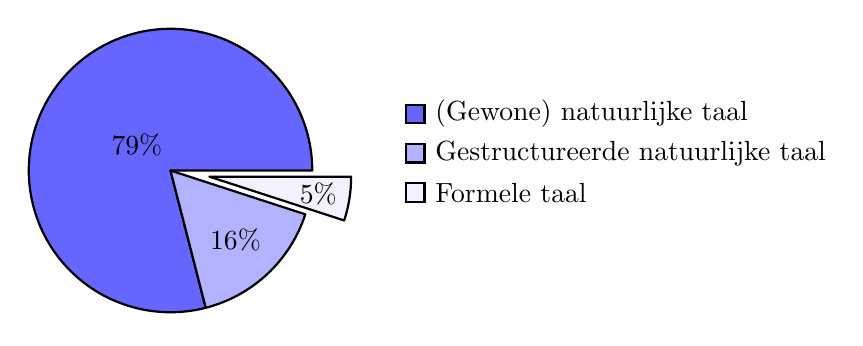
\begin{tikzpicture}
      \pie[text = legend, radius = 1.8, explode = {0, 0, 0.5}, color = {blue!60, blue!30, blue!5}]{79/(Gewone) natuurlijke taal, 16/Gestructureerde natuurlijke taal, 5/Formele taal}
  \end{tikzpicture}
  \caption[Gebruik van natuurlijke taal in vereistenanalyse]{Gebruik van natuurlijke taal in vereistenanalyse in 1999 (van figuur 5 in \cite{Luisa2004})}
  \label{fig:natural-language-use}
\end{figure}

We kozen voor logigrammen als eerste stap in het onderzoek naar zo'n formele natuurlijke taal. Dit omwille van het feit dat logigrammen reeds een beperkte set van zinsconstructies bevat. Bovendien is de evaluatie makkelijker omwille van de veelheid aan logigrammen die men kan vinden.


% Nu begint de eigenlijke tekst
\mainmatter
\chapter{Achtergrond}
Om deze thesis te begrijpen worden hier een aantal concepten uitgelegd die niet per se tot de achtergrondkennis behoren van de lezer. Definite Clause Grammars zijn een soort van grammatica die een aantal voordelen biedt voor het parsen van natuurlijke taal. Feature structures zorgen voor een beperking van het aantal grammaticale regels en verhogen de leesbaarheid ervan. Discourse Representation Theory is een theorie uit de taalkunde voor het vatten van de betekenis van taal. Het introduceert Discourse Representation Structures, een logica die dichter aanleunt bij de natuurlijke taal.

\section{Definite Clause Grammars}
\label{sec:DCG}
Definite Clause Grammars \cite{Pereira1980} zijn een uitbreiding van contextvrije grammatica's die vaak ingebakken zitten in logische talen zoals prolog. Pereira et al.\ \cite{Pereira1980} geven 3 voorbeelden van hoe DCG's kunnen helpen bij het parsen van natuurlijke talen:

\begin{enumerate}
  \item De woordvorm kan afhankelijk gemaakt worden van de context waarin deze verschijnt. Zo kan men eisen dat een werkwoord in de juiste vervoeging voorkomt.
  \item Tijdens het parsen kan men een boom opbouwen die de semantiek van de zin moet vatten. Deze boom hoeft niet isomorf te zijn met de structuur van de grammatica.
  \item Het is mogelijk om prolog code toe te voegen die extra restricties oplegt aan de grammatica.
\end{enumerate}

\subsection{Een eerste grammatica}
\begin{ex}
  Een voorbeeld van een DCG grammatica is:
  \begin{quote}
    \texttt{s ---> np, vp.} \\
    \texttt{np ---> [ik].} \\
    \texttt{np ---> [hem].} \\
    \texttt{vp ---> v, np.} \\
    \texttt{v ---> [zie].}
  \end{quote}
\end{ex} 
\texttt{s} is het startsymbool en staat voor \texttt{sentence}. \texttt{np} staat voor \texttt{noun phrase} (naamwoordgroep of nominale constituent), \texttt{vp} voor \texttt{verb phrase} (verbale constituent) en \texttt{v} voor \texttt{verb}. Deze grammatica zegt dat een zin bestaat uit een noun phrase gevold door een verb phrase. Een verb phrase is dan weer een werkwoord gevolgd door een noun phrase.

De zin \example{ik zie hem} is onderdeel van deze taal. Maar ook de zin \example{ik zie ik} is deel van de taal. Om dit op te lossen kunnen we argumenten meegeven aan de niet-terminaal \texttt{np}.

\subsection{De woordvorm is afhankelijk van de context}
\begin{ex}
  \label{ex:nom-acc-features}
  Deze verbeterde grammatica houdt rekening met welke woordvorm kan voorkomen in welke context.
  \begin{quote}
    \texttt{s ---> np(nom), vp.} \\
    \texttt{np(nom) ---> [ik].} \\
    \texttt{np(acc) ---> [hem].} \\
    \texttt{vp ---> v, np(acc).} \\
    \texttt{v ---> [zie].} \\
  \end{quote}
\end{ex} 

De \texttt{nom} en \texttt{acc} slaan hier op de naamvallen \texttt{nominatief} en \texttt{accusatief}. Ze geven aan in welke functie de naamwoordgroepen gebruikt mogen worden binnen een zin.

\subsection{Een boom als resultaat}
\begin{ex} Verder is het ook mogelijk om een boom op te bouwen tijdens het parsen.
  \begin{quote}
    \texttt{s(Tree) ---> np(NP, nom), vp(Tree, NP).} \\
    \texttt{np(ik, nom) ---> [ik].} \\
    \texttt{np(hem, acc) ---> [hem].} \\
    \texttt{vp(Tree, Subject) ---> v(Tree, Subject, Object), np(Object, acc).} \\
    \texttt{v(zien(Subject, Object), Subject, Object) ---> [zie].}
  \end{quote}
\end{ex} 

Bij het parsen van \example{ik zie hem} krijgen we nu volgende boom:

\Tree[.\textit{zien} \textit{ik} \textit{hem} ]

Merk op dat deze boom de structuur van de grammatica niet hoeft te volgen. Het werkwoord wordt hier tot belangrijkste woord van de zin gebombardeerd.

\subsection{Prolog-code in de grammatica}
\begin{ex} Ten slotte is het mogelijk om prolog restricties te embedden in de grammatica door deze prolog goals tussen accolades te plaatsen.
  \begin{quote}
    \texttt{expression(X) ---> factor(X).} \\
    \texttt{expression(X) ---> term(X).} \\

    \texttt{factor(X) ---> numeral(X).} \\
    \texttt{factor(X) ---> numberal(A), [*], factor(B), \{X is A * B\}.} \\
    \texttt{term(X) ---> factor(A), [+], expression(B), \{X is A + B\}.} \\

    \texttt{numeral(X) ---> [X], \{number(X)\}.} \\
  \end{quote}
\end{ex} 

Bovenstaande grammatica kan simpele wiskunde expressies omvormen tot de wiskundige waarde. Zo wordt \texttt{2 + 4 * 5} omgevormd tot \texttt{22} volgens volgende boom. Hierbij wordt de waarde van onder uit de boom naar boven toe gepropageerd via unificatie.

\Tree[.expression(22)
        [.term(22) [.factor(2) [.number(2) 2 ]]
                   +
                   [.expression(20) [.factor(20) [.number(4) 4 ] * [.factor(5) [.number(5) 5 ]]]]]]

De prologcode in de accolades heeft twee functies. Enerzijds berekent die de waarde van een subexpressie zoals een factor of een term. Anderzijds beperkt de prologcode de grammatica. Een \texttt{numeral} bestaat uit 1 token maar enkel als dat token een getal is volgens prolog. Zo'n beperking in prolog kan ook gebruikt worden om uit de beperkingen van een contextvrije grammatica te treden.

\subsection{Conclusie}
\paragraph{} Definite Clause Grammars zijn expressieve grammatica's die uitermate geschikt zijn voor het modelleren van de grammatica van een natuurlijke taal. In deze thesis zullen alle grammatica's dan ook gegeven worden in de vorm van een DCG.

% \paragraph{}Een laatste opmerking bij deze grammatica is de asymmetrische vorm voor factoren en termen. Een factor is bijvoorbeeld niet gedefinieerd als de vermenigvuldiging van 2 factoren. Dit komt omdat DCG's niet enkel definities zijn van grammatica's maar ook een uitvoeringsstrategie hebben. M.a.w. men krijgt er gratis een parser bij. Deze parser werkt, net als prolog, top-down en van links naar rechts. In het geval van links recursieve regels, zou de parser in een oneindige lus kunnen geraken. Het is echter een bekend resultaat dat men een grammatica altijd kan omvormen zodat deze niet langer links recursief is. Dit is dus geen beperking op welke talen voorgesteld kunnen worden.

% \paragraph{} DCG's zonder prolog code zijn zeer declaratief. Men kan ze namelijk ook puur als definitie van een grammatica beschouwen. Zo kan men een chart parser schrijven die gebruik maakt van een DCG als definitie van de grammatica. Chart parsers zijn interessant voor CNL's omdat ze onthouden welke parti\"ele en volledige constituenten ze al gevonden hebben \cite{Kuhn2008}. Daardoor is er geen nood aan backtracking. Men moet zo niet telkens opnieuw bewijzen wat in een andere tak al bewezen was. Een chart parser onthoudt dat \example{een man} een naamwoordgroep is en kijkt hoe het deze woordgroep kan combineren met andere woorden tot parti\"ele of volledige constituenten. Daardoor is een chart parser veel sneller dan de gratis parser van prolog.

% Bovendien kan men uit de parti\"ele constituenten afleiden welke woordcategorie\"en kunnen volgen op een parti\"ele zin. Zo kan de parti\"ele zin \example{Een rode} gevolgd worden door een adjectief of substantief maar niet door een lidwoord of een werkwoord. Op basis hiervan kan men een suggestietool maken die suggesties geeft i.v.m.\ welke woorden kunnen volgen.

% Ten slotte kan men bij het toevoegen van een woord aan een parti\"ele zin, de resultaten van de vorige parse gebruiken. Dit levert een extra performantiewinst op t.o.v.\ de gratis parser in het geval van incrementele parses. Dit is vooral interessant tijdens het schrijven van een zin, waarbij de vorige parti\"ele zin steeds wordt uitgebreid met \'e\'en woord. Een chart parser hoeft in dat geval namelijk enkel te kijken naar dit nieuwe woord en naar wat er in het geheugen is van de vorige parse, niet meer naar de andere woorden in de zin.

\section{Feature structures}
\label{sec:featureStructures}

\paragraph{} Een feature structure is een term uit de taalkunde. Men kan ze zien als \textit{named arguments} voor een niet-terminaal die gebruikt worden om een explosie aan grammaticale regels te voorkomen. Zo kan een \texttt{np} en \texttt{vp} een feature \texttt{getal} hebben dat aangeeft of de woordgroep in het enkelvoud of meervoud staat. De grammaticale regel voor een zin kan dan aangeven dat het onderwerp en werkwoord moeten overeenkomen in getal. Andere features geven bijvoorbeeld de naamval aan van een naamwoordgroep. Blackburn en Striegnitz \cite{NLPCourse} geven de volgende grammaticale regel als voorbeeld (hierbij staat \texttt{CAT} voor de categorie van een woordgroep):

\[
  \fstructure{
    \feature{CAT}{s}
  }
  \rightarrow
  \fstructure{
    \feature{CAT}{np}
    \feature{NAAMVAL}{nom}
    \feature{GETAL}{\fvariable{1}}
  }
  \fstructure{
    \feature{CAT}{vp}
    \feature{GETAL}{\fvariable{1}}
  }
\]

Deze regel zegt dat een zin bestaat uit een \texttt{np} gevolgd door een \texttt{vp}. De \texttt{np} moet de naamval \texttt{nom} hebben. Bovendien moet het getal van de \texttt{np} en de \texttt{vp} unificeren (de \framebox{1} kan men zien als een variabele).

Grammatica's die gebruik maken van feature structures, gebruiken altijd unificatie voor het samenvoegen van meerdere structuren. Niet alle features moeten namelijk altijd een waarde toegekend krijgen. Zo kan een eigennaam voorkomen als onderwerp en als lijdend voorwerp (en heeft dus geen waarde voor de feature \texttt{naamval}). Terwijl \example{ik} enkel als onderwerp kan voorkomen (en dus wel een waarde heeft voor die feature). Zoals in het voorbeeld hierboven kan men door unificatie ook controleren of meerdere woordgroepen dezelfde waarden hebben voor een feature.

\paragraph{} Zoals Shieber et al.\ \cite{Shieber2003} aanhalen, verschillen prolog termen van feature structures enkel in vorm. Zo speelt de volgorde in prolog wel een rol. Ten slotte moet men steeds alle features vermelden, ook als ze ongebonden zijn. Qua expressiviteit voegen ze echter niets toe aan DCG's. Zo is bovenstaande grammaticale regel op basis van feature structures equivalent met volgende DCG-regel:

\[
    \texttt{s ---> np([naamval:nom, getal:Getal]), vp([getal:Getal]).} \\
\]

\paragraph{} Feature structures (en argumenten in DCG's) zijn handig om de explosie van grammatica regels te voorkomen.
\begin{ex}  Een voorbeeld van een grammatica zonder feature structures uit \cite{NLPCourse}:
  \label{ex:explosion}
  \begin{quote}
    \texttt{s ---> np\_{singular}, vp\_{singular}.} \\
    \texttt{s ---> np\_{plural}, vp\_{plural}.} \\
    \texttt{np ---> np\_{singular}.} \\
    \texttt{np ---> np\_{plural}.} \\
    \texttt{np\_{singular} ---> det, n\_{singular}.} \\
    \texttt{np\_{plural} ---> det, n\_{plural}.} \\
    \texttt{vp\_{singular} ---> intransitive\_verb\_{singular}.} \\
    \texttt{vp\_{singular} ---> transitive\_verb\_{singular}, np.} \\
    \texttt{vp\_{plural} ---> intransitive\_verb\_{plural}.} \\
    \texttt{vp\_{plural} ---> transitive\_verb\_{plural}, np.} \\
    \texttt{n\_singular ---> [man].} \\
    ...
  \end{quote}
\end{ex} 
Hierbij staat de \texttt{n} voor zelfstandig naamwoord (van het Engelse \texttt{noun}) en \texttt{det} voor determinator. Deze grammatica can veel korter gemaakt worden door gebruik te maken van feature structures:

\begin{ex}  Een grammatica met feature structures equivalent aan voorbeeld \ref{ex:explosion} (ook uit \cite{NLPCourse})
  \begin{quote}
    \texttt{s ---> np([num:Num]), vp([num:Num]).} \\
    \texttt{np([num:Num]) ---> det, n(num:Num).} \\
    \texttt{vp([num:Num]) ---> intransitive\_verb([num:Num]).} \\
    \texttt{vp([num:Num]) ---> transitive\_verb([num:Num]), np(\_).} \\
    \texttt{n([num:singular]) ---> [man].} \\
    ...
  \end{quote}
\end{ex} 

\paragraph{Conclusie} Door gebruik te maken van feature structures is de grammatica simpeler en leesbaarder. Bovendien hoeft het concept dat een zin bestaat uit een \texttt{np} gevolgd door een \texttt{vp} maar \'e\'en keer te worden uitgedrukt. De feature structures zorgen voor de congruentie in getal van het onderwerp met het werkwoord.

\section{Discourse Representation Theory}
Voor het vertalen van natuurlijke taal naar logica zouden we graag gebruik maken van Frege's compositionality principe: De betekenis van een zin bestaat uit de combinatie van de betekenissen van de delen ervan. Als we eerste-orde-logica als doeltaal van onze vertaling nemen, komen we echter vrij snel in de problemen. Neem bijvoorbeeld de zin ``If a man lives, he breathes''. De vertaling hiervan in eerste-orde-logica is $\forall x. man(x) \Rightarrow breath(x)$. De vertaling van ``a man lives'' is echter $\exists x. man(x)$, wat geen deel uit maakt van de betekenis van de hele zin. Blackburn en Bos \cite{Blackburn2006} geven nog een aantal andere voorbeelden waarvoor DRS-structuren beter geschikt zijn dan eerste-orde-logica (bijvoorbeeld voor het oplossen van anaforische referenties).

Ze suggereren Discourse Representation Structures als alternatief. Deze structuren bestaan uit een lijst van \textit{discourse referents} (woordgroepen waarnaar andere woordgroepen kunnen verwijzen) en een lijst van condities i.v.m. die referenties \cite{Bos2011}. Blackburn en Bos \cite{Blackburn2006} geven o.a. een vertaling van deze DRS-structuren naar eerste-orde-logica. DRS-structuren hebben dus ook een formele betekenis, zoals we verder zullen aantonen, zijn ze echter beter geschikt als doeltaal. Van hieruit kan dan verder vertaald worden naar eerste-orde-logica volgens de vertaling van Blackburn en Bos. Wij hernemen hier hun vertaling als verdere introductie tot deze structuren:

\[
\Bigg(\drs{x_1, ..., x_n}{
  \gamma_1 \\
  ... \\
  \gamma_n
}\Bigg)^{fo} = \exists x_1...\exists x_n\Big((\gamma_1)^{fo} \land ... \land (\gamma_n)^{fo}\Big)
\]

En de vertaling van alle mogelijke condities:

\[\Big(R(x_1, ..., x_n)\Big)^{fo} = R(x_1, ..., x_n)\]
\[\Big(\tau_1 = \tau_2\Big)^{fo} = \Big(\tau_1 = \tau_2\Big)\]
\[\Big(\lnot B)^{fo} = \lnot\Big(B\Big)^{fo}\]
\[\Big(B_1 \lor B_2)^{fo} = \Big(B_1\Big)^{fo} \lor \Big(B_2\Big)^{fo}\]

\[\Big(\drs{x_1, ..., x_n}{\gamma_1 \\ ... \\ \gamma_2} \Rightarrow B\Big)^{fo} =  \forall x_1...\forall x_n\Bigg(\Big((\gamma_1)^{fo} \land ... \land (\gamma_n)^{fo}\Big) \Rightarrow \Big(B\Big)^{fo} \Bigg)\]

De vertaling van ``If a man lives, he breathes'' naar DRS is \\

\drs{}{\ifdrs{X}{man(X) \\ lives(X)}{}{breathes(X)}}

\paragraph{} Merk op dat de betekenis van het deel ``a man lives'' \drs{X}{man(X) \\ lives(X)} wel deel uitmaakt van de betekenis van de hele zin.

\section{Conclusie} Definite Clause Grammars vormen een expressieve grammatica die natuurlijke taal in al haar facetten makkelijk kan modelleren. Feature Structures komen overeen met argumenten in prolog en kunnen gebruikt worden om grammatica's kort en leesbaar te houden. Discourse Representation Structures vormen een representatie die tussen natuurlijke taal en eerste-orde-logica ligt. Ze zijn even expressief als eerste-orde-logica maar een aantal concepten in de natuurlijke taal zijn beter te modelleren met DRS-structuren.


\chapter{Related work}
In het verleden zijn er al meerdere CNL's gemaakt. Sommige zijn ontwerpen om de leesbaarheid van de specificaties te verhogen en hebben geen formele semantiek. Kuhn \cite{Kuhn2014} heeft een classificatieschema ontwerpen voor CNL's genaamd PENS: \texttt{Precision} (hoe ambigu/formeel is de taal), \texttt{Expressivity} (welke problemen kunnen we uitdrukken), \texttt{Naturalness} (hoe vlot leest de taal), \texttt{Simplicity} (hoe simpel is de taal). In dezelfde paper lijst Kuhn ook een heleboel CNL's op met hun geschiedenis en nut alsook hun classificatie volgens het PENS-schema.

Meer in het algemeen is het omvormen van teksten in natuurlijke taal tot formele modellen al gebeurd in verschillende domeinen: in vereistenanalyse, in het paradigma van business rules, binnen de computationele lingu\"istiek en ten slotte in het domein van de kennisrepresentatie.

Deze sectie geeft een kort overzicht van wat er al gebeurd is in al deze domeinen. Voor een completer overzicht van CNL's, verwijzen we naar Kuhn \cite{Kuhn2014}.

\section{Vereistenanalyse}
\paragraph{Circe} De tool Circe \cite{Ambriola1997} wordt gebruikt in vereistenanalyse. De gebruiker moet een vocabularium, een set van substitutieregels en een specificatie in natuurlijke aanleveren. De tool probeert dan steeds de beste substitutieregel te vinden om zo de tekst geleidelijk aan te transformeren naar een formeel model. Het grote voordeel van de methode is dat er regelsets bestaan voor meerdere soorten modellen: data flow modellen, entity-relationship modellen, ...

Verder is het in Circe mogelijk om in het vocabularium woorden te taggen. De regels kunnen hier dan gebruik van maken om te bepalen of ze van toepassing zijn op bepaalde zinnen. Op die manier introduceert Circe types in het vocabularium.

Een voorbeeld (uit \cite{Ambriola1997}): \example{bron/UIT STUURT data/INFO NAAR doel/IN}. De woorden \example{stuurt} en \example{naar} liggen vast in de regelset. De andere 3 woorden komen uit het vocabularium. Deze moeten een bepaalde tag hebben om te matchen met de regel. Er zijn dus drie types in deze zin: entiteiten die informatie kunnen versturen, entiteiten die informatie kunnen ontvangen en informatie die verzonden kan worden.

Circe is niet echt een CNL. Zinnen die niet matchen met een substitutieregel worden ook niet omgezet in een formeel model. De specificatie kan dus zinnen met en zonder formele betekenis mengen. Er is geen sprake van constructieregels. Alleen (delen van) zinnen die matchen met een substitutieregel krijgen een formele betekenis.

\section{Business rules}
Binnen het paradigma van business rules spelen zowel natuurlijke talen als formele talen een grote rol. SBVR Structured English (SBVR-SE) \cite{Levy2013} en RuleSpeak \cite{Ross2009a} zijn 2 CNL's die proberen om ambigu\"iteit in de natuurlijke taal te verminderen. Deze talen focussen echter vooral op het menselijke aspect \cite{Njonko2014}. Het doel van deze talen is om ambigu\"iteit uit de specificatie te halen en niet zozeer om automatisch natuurlijke taal om te zetten naar een formele voorstelling. RuleCNL \cite{Njonko2014} heeft wel dit doel.

RuleCNL splitst de specificatie op in twee delen: een vocabularium en de regels zelf. Het vocabularium bestaat uit substantieven en werkwoorden alsook hoe deze in verhouding staan tot elkaar. Bijvoorbeeld \example{Auto heeft wiel} geeft aan dat er een relatie kan bestaan tussen een auto en een wiel. Het vocabularium in RuleCNL is dus getypeerd. Voor de regels zelf bestaat er een contextvrije grammatica waaraan de zinnen moeten voldoen.

Om de gebruikers te helpen bij het schrijven van de zinnen in RuleCNL, is er een plug-in voor de Eclipse IDE die automatisch zinnen kan aanvullen en de structuur van bestaande zinnen aangeeft door het kleuren ervan. Bovendien is er een visuele representatie van het domein om de gebruiker te helpen bij het schrijven van het vocabularium.

\section{Computationele lingu\"istiek} Er zijn reeds 2 belangrijke CNL's opgesteld die vertaald kunnen worden naar formele modellen: Attempto Controlled English (ACE) en Processable English (PENG). Beide talen lijken op elkaar en hebben gelijkaardige tools om mee te werken. Ze komen ook allebei uit de computationele lingu\"istiek en zijn ingebakken in taalkundige frameworks die gemaakt zijn om de semantiek van natuurlijke taal in het algemeen te vatten. In de papers over ACE en PENG wordt er niet zoveel gesproken over deze taalkundige aspecten omdat een achtergrond in de (computationele) lingu\"istiek verondersteld wordt.

Hierna volgt eerst een bespreking van ACE. Daarna bespreken we PENG. Hierbij ligt de nadruk op de gelijkenissen en verschillen met ACE. We sluiten af met een beschrijving van hoe deze twee talen ge\"implementeerd zijn met een nadruk op de verduidelijking van een aantal taalkundige aspecten die amper aan bod komen in de papers over ACE en PENG.

\subsection{Attempto Controlled English (ACE)}
\paragraph{} Attempto Controlled English \cite{Fuchs2008} is een gestructureerde natuurlijke taal voor kennisrepresentatie. Het is een subset van Engels die naar een subset van eerste-orde-logica vertaalt. Het is een formele taal: elke zin in ACE heeft slechts \'e\'en betekenis, ook al is de zin ambigu in het Engels. Om te bepalen welke van de betekenissen de \textit{correcte} betekenis is, moet men de interpretatieregels volgen. Omdat dit soms nogal ingewikkeld is, kan men gebruik maken van de parafraseertool van ACE. Deze tool zet de interne representatie terug om naar \'e\'en of meerdere zinnen in ACE. Op die manier kan men niet alleen de betekenis van de zin leren, maar ook de taal zelf. Deze parafrasering leunt echter zeer nauw aan bij de formele taal. Hierdoor is ze niet altijd toegankelijk voor iemand zonder een achtergrond in formele talen.

Bijvoorbeeld de zin \example{Everybody is not present.} heeft 2 betekenissen in het Engels: \example{Everybody is absent} en \example{Somebody is absent}. In ACE is de eerste betekenis de \textit{correcte}. Deze zin wordt geparafraseerd als \example{If there is somebody X1 then it is false that X1 is present.} \footnote{De parafrasering komt van de Attempto Parsing Engine (http://attempto.ifi.uzh.ch/ape/)}. Dit is al een vrij moeilijke parafrasering om te begrijpen terwijl de originele zin nog redelijk simpel is.

\paragraph{}ACE is een general purpose CNL: Het bevat een ingebouwd vocabularium. De gebruiker moet dus zelf geen vocabularium opstellen en kan direct beginnen met het schrijven van de specificatie. Het nadeel aan deze aanpak is dat ACE dus ook geen domeinkennis kan gebruiken voor het analyseren van de zinnen. Sommige constructies moeten daarom met een koppelteken geschreven worden. Zo wordt er in \cite{ACEConstructionRules} het voorbeeld gegeven van \example{A student is interested-in a course} en \example{A student is interested in a classroom}.

Op die manier probeert ACE sommige ambigu\"iteiten op te lossen. Een gelijkaardige truc wordt bijvoorbeeld ook gebruikt om de voorrang van \example{en} en \example{of} op te lossen. Standaard heeft \example{en} voorrang. Maar als de \example{en} voorafgegaan wordt door een komma, dan heeft \example{of} voorrang. \cite{ACEConstructionRules} geeft het voorbeeld \example{A client \{enters a red card or enters a blue card\}, and enters a code.}

In andere gevallen kiest ACE gewoon hoe de zin ge\"interpreteerd moet worden op basis van een set van interpretatieregels. Zo slaat de \example{manually} in \example{A customer who {enters a card manually} types a code.} \cite{ACEConstructionRules} op \example{enters} en niet op \example{types} omdat een bijwoord bij voorkeur achter het werkwoord staat. (De parafrasering is in dit geval wel makkelijk te begrijpen maar vrij lang: \example{There is a customer X1. The customer X1 types a code. The customer X1 enters a card manually.}). Merk ook op dat het onbepaalde lidwoord aanleiding geeft tot een existenti\"ele quantor. In dit geval is de universele quantor echter beter geschikt.

\paragraph{} \'E\'en van de sterke punten van ACE is haar coreferentie-analyse. Dit is het onderzoeken van welke woordgroepen naar hetzelfde concept verwijzen. Neem bijvoorbeeld de zinnen \example{Een man heeft een vrouw. Hij is gelukkig.}. Hierin is \example{Hij} een anaforische referentie (een referentie naar een woordgroep die eerder komt) naar \example{een man}. ACE kan deze coreferenties correct analyseren. ACE doet dit door haar embedding in Discourse Representation Theory, een taalkundig framework. Men kan hier redelijk ver in gaan. Zo worden de zinnen \example{There is a red house and there is a blue house. The red house is large.} correct geanalyseerd. Doordat zinnen in ACE als \'e\'en geheel vertaald worden, kan men dus lange zinnen met veel bijzinnen herschrijven in meerdere kortere zinnen. Dit kan de leesbaarheid van een specificatie vergroten.

\paragraph{} Origineel was ACE bedoeld voor het opstellen van specificaties voor software. Ondertussen kent de taal al meerdere toepassingen, in verschillende domeinen. Er zijn ook meerdere tools die overweg kunnen met ACE als input.

Zo is er de Attempto Parsing Engine APE die ACE zinnen omzet naar Discourse Representation Structures. Dit zijn datatypes uit Discourse Representation Theory die de semantiek van de zin bevatten. APE geeft ook een parafrasering van de invoertekst. Zodat de gebruiker kan controleren of de tool de tekst op de juiste manier leest. Bovendien kan APE waarschuwingen geven bij mogelijke problemen. Bijvoorbeeld het gebruik van een anaforische referentie zonder een antecedent waarnaar deze anafoor kan verwijzen.

\paragraph{} Verder is er de Attempto Reasoner RACE. Deze tool kan controleren of een specificatie consistent is. Indien niet, zal de tool zeggen welke zinnen met elkaar in conflict zijn. Op die manier weet de gebruiker dat er een fout is en waar deze zich ongeveer bevindt. Daarnaast kan de tool vragen in natuurlijke taal beantwoorden. RACE antwoordt niet alleen op de vraag maar geeft ook de zinnen die nodig zijn om te bewijzen dat het gegeven antwoord juist is. Ten slotte kan RACE bewijzen of een bepaalde zin het logische gevolg is van de specificatie. Op die manier kan de gebruiker testen of de specificatie correct is.

APE en RACE zijn de twee belangrijkste tools. Er zijn er echter nog veel meer. Zo is er de ACE View Prot\'eg\'e plug-in. Dit is een plug-in die de vertaling tussen Web Ontology Language (OWL) en ACE doet binnen de Prot\'eg\'e-omgeving (een editor voor het maken van ontologi\"en). Op die manier ziet de gebruiker enkel ACE zinnen en hoeft dus de formele OWL taal niet te kennen om met bestaande modellen om te gaan of om nieuwe modellen te maken. Ten slotte is er AceRules. Hiermee kan de gebruiker de zinnen die ge\"impliceerd worden door de specificatie te weten komen.

Over het algemeen is ACE een zeer uitgebreide taal. Veel Engelse zinnen zijn geldige ACE zinnen, echter niet allemaal. Hierdoor is het moeilijk om de taal te leren. Het is immers niet super duidelijk wat toegestaan is en wat niet. Volgens Fuchs et al.\ \cite{Fuchs2008} heeft een gebruiker 2 dagen nodig om de taal te leren.

\subsection{Processable English (PENG)}
\paragraph{} Andere talen zoals PENG \cite{Schwitter2002} zijn makkelijker om te leren dan ACE. PENG is net als ACE een CNL die vertaalt naar DRS-structuren. In tegenstelling tot ACE bevat PENG geen groot ingebouwd lexicon. De gebruiker moet zelf de woorden aanbrengen die gebruikt worden. De gebruiker kan dit doen tijdens het bewerken en moet dus niet op voorhand aangeven wat het lexicon is. De categorie\"en voor deze domeinspecifieke woorden zijn substantief, adjectief, werkwoord of bijwoord. PENG biedt ook de mogelijkheid om synoniemen of afkortingen te introduceren. Op die manier kan de specificatie vlotter gemaakt worden. Men kan echter geen types meegeven in het lexicon. Men kan dus niet zeggen dat het werkwoord \example{ademen} enkel uitgevoerd kan worden doormensen of dieren en niet door objecten. Naast de domeinspecifieke woorden kent PENG een aantal functionele woorden die ingebakken zitten in de taal, zoals lidwoorden en voegwoorden (\example{de man \underline{die}}). Deze woorden helpen PENG om de zinsconstructies te herkennen.

Net zoals ACE kent PENG het principe van constructieregels en interpretatieregels. De constructieregels bepalen welke zinnen deel zijn van de taal. Bij PENG zijn deze regels eenvoudiger omdat de taal zeer simpel gehouden is. Hierdoor is het makkelijker om zinnen te maken in de taal. Over het algemeen lijken de constructieregels van PENG en ACE veel op elkaar.

De interpretatieregels bepalen hoe de zin vertaald wordt naar logica. Zo is er een interpretatieregel voor hoe anaforische referenties opgelost worden. Deze regel is gelijkaardig in ACE en PENG. Andere regels bepalen welke functiewoorden sterker binden. Zowel ACE als PENG gebruiken hiervoor dezelfde volgorde als in eerste-orde-logica. ACE staat wel uitzonderingen toe door het toevoegen van komma's. PENG houdt de taal simpel en staat dit niet toe.

\paragraph{} PENG is makkelijker om te leren dan ACE omwille van ECOLE \cite{Schwitter2003}. Een tool die suggesties geeft over de woordcategorie\"en die kunnen volgen op een bepaalde zin. Zo geeft Schwitter \cite{Schwitter2003} het voorbeeld van \example{Een} dat gevolgd kan worden door een \texttt{adjectief} of een \texttt{substantief}. Indien de gebruiker de woordcategorie niet kent, kan hij doorklikken op die categorie voor een aantal concrete mogelijkheden. Op die manier moet de gebruiker enkel de woordcategorie\"en leren en niet de geldige zinsconstructies.

Naast de suggestietool bestaat er voor PENG, net zoals voor ACE, ook een parafraseertool. Deze tool herschrijft de invoer zodat het duidelijker is hoe PENG de zin begrepen heeft. Anaforische referenties worden bijvoorbeeld omgezet in de naamwoordgroep waarnaar ze verwijzen.

Net zoals voor ACE zinnen is het ook voor een PENG zinnen mogelijk om te controleren of ze een consistente specificatie vormen \cite{Schwitter2004b}. Daarnaast is het mogelijk om te controleren op redundantie. Indien een zin al door een andere zin ge\"impliceerd wordt, hoeft deze niet expliciet deel uit te maken van de specificatie. Op die manier kan de specificatie kort gehouden worden, wat de leesbaarheid verhoogd.

Naast de general purpose CNL bevat PENG ook een subset specifiek voor het semantische web: PENG-D \cite{Schwitter2004}. Deze subset kan vertaald worden naar description logic (OWL DL), een subset van eerste-orde-logica. PENG-D kan dus gezien worden als het alternatief voor de ACE View Prot\'eg\'e plug-in.
Schwitter \cite{Schwitter2006} vermeldt drie klassieke manieren van voorstellen van een ontologie (N-Triples, RDF/XML en OWL Abstract) en toont dan verder aan dat PENG een vierde manier is om hetzelfde voor te stellen. De paper toont dit aan door verschillende constructies uit OWL te mappen op zinnen in PENG. Het grote voordeel van PENG t.o.v. de andere voorstellingswijzen is dat PENG ook leesbaar en begrijpbaar is voor de mens.

\subsection{Implementatie}
\paragraph{} Zowel ACE als PENG zijn ge\"implementeerd in prolog met behulp van Definite Clause Grammars (DCG) en feature structures voor het omzetten van de natuurlijke taal naar DRS-structuren \cite{Fuchs2008, Schwitter2006}.

\paragraph{Definite Clause Grammars} Aangezien zowel ACE als PENG gebruiken maken van prolog voor hun (eerste) implementatie, is de keuze voor DCG's voor de hand liggend omwille van de parser die men er gratis bijkrijgt. In de tools voor ACE en PENG wordt er echter gebruik gemaakt van een chart parser. Deze parser kan tijdens het schrijven van de zinnen, heel snel voorspellen welke woordcategorie\"en kunnen volgen. Dit helpt de gebruiker bij het schrijven van grammaticaal correcte zinnen zonder de taal te moeten kennen. PENG gebruikt zo'n chart parsers in ECOLE \cite{Schwitter2003}. ACE heeft in navolging van PENG ook AceWiki \cite{Kuhn2008} gemaakt, een subset van ACE voor semantische wiki's. Ook AceWiki bevat een suggestietool. Kuhn et al.\ \cite{Kuhn2008} leggen in detail uit hoe zo'n chart parser gemaakt kan worden voor een CNL en vergelijken de performantie van deze parsers met de gratis parser van prolog.

\paragraph{Feature structures} Naast DCG's wordt er in ACE en PENG ook gebruikt gemaakt van feature structures \cite{Shieber2003, NLPCourse}. Binnen ACE en PENG zorgen de feature structures voor de syntactische correctheid van de zinnen in de gasttaal, het Engels. Via unificatie kan men namelijk testen of een bepaalde woordgroep voldoet aan de voorwaarden van de context. De unificatie van de feature \texttt{getal} van het onderwerp en het werkwoord zorgt voor de congruentie in getal van het onderwerp met het werkwoord. Op die manier zijn zinnen die in ACE en/of PENG geldig zijn, ook geldig in het Engels. Zoals sectie \ref{sec:featureStructures} aanhaalt, wordt op deze manier een explosie van het aantal grammaticale regels vermeden.

\paragraph{DRS} Naast feature structures maken ACE en PENG ook gebruik van Discourse Representation Structures. Ze zijn een onderdeel van Discourse Representation Theory. Dit is een taalkundig framework om de semantiek van natuurlijke taal te vatten. Één van de sterke punten van DRS-structuren is het oplossen van coreferenties. \cite{Fuchs2008drs} bevat meer informatie over hoe DRS-structuren gebruikt worden binnen ACE.

Bos \cite{Bos2011} stelt dat DRS-structuren zowel de rol van semantische inhoud als die van tekstuele context spelen. M.a.w.\ met behulp van deze structuren kan men achterhalen wat de semantiek van een tekst is maar tegelijk bieden ze ook een context aan die helpt bij de coreferentie-analyse. Zo wordt tijdens het parsen de semantiek van een zin opgebouwd en tegelijk de coreferenties opgelost.

Concreet bevat een DRS-structuur een lijst van \textit{discourse referents} (woordgroepen waarnaar andere woordgroepen kunnen verwijzen) en een lijst van bepaling i.v.m. die referenties \cite{Bos2011}. \autoref{drs:example} geeft een voorbeeld van zo'n DRS-structuur voor de zin \example{There is a movie which every man loves deeply}. Er zijn in totaal 3 \textit{discourse referents}: \texttt{movie}, \texttt{man} en \texttt{loves}. Merk op dat naar deze laatste verwezen wordt door het bijwoord \textit{deeply}. Deze DRS kan vertaald worden als $\exists A \cdot \bigg(movie(A) \land \forall B \cdot \Big(man(B) \Rightarrow \exists C \cdot \big( loves(C, B, A) \land deeply(C) \big)\Big)\bigg)$

\begin{savenotes}
  \begin{drsFloat}
    \centering
    \drs{A}{
      movie(A) \\
      \ifdrs{B}{man(B)}
            {C}{loves(C, B, A) \\ deeply(C)}
    }
    \caption{Een DRS-structuur voor de zin \example{There is a movie which every man loves deeply.} \protect\footnotemark}
    \label{drs:example}
    \footnotetext{Deze DRS-structuur werd lichtjes aangepast aan de output van APE (http://attempto.ifi.uzh.ch/ape/)}
  \end{drsFloat}
\end{savenotes}


\paragraph{Conclusie} DCG's zijn een uitbreiding op contextvrije grammatica's uit de wereld van logisch programmeren. Feature structures en Discourse Representation Structures zijn concepten uit de lingu\"istiek. Ze worden gebruikt om de natuurlijke taal en haar semantiek te modelleren. Zo helpen feature structures om een explosie van het aantal grammatica regels te voorkomen. Discourse Representation Structures worden dan weer vooral gebruikt om de coreferentie-analyse te vergemakkelijken. Beiden concepten worden gebruikt in de tools rond ACE en PENG omdat deze talen ontstaan zijn in het vakgebied van computationele lingu\"istiek.

\section{Kennisrepresentatie}
\label{sec:ASP}
In het domein van kennisrepresentatie hebben Baral et al.\ \cite{Baral2008} natuurlijke taal reeds vertaald naar Answer Set Programs (ASP). Ze maken hiervoor gebruik van Combinatorische Categorische Grammatica (CCG) en $\lambda$-calcalus. Een CCG bestaat uit een aantal basiscategorie\"en zoals \texttt{s} (zin) en \texttt{np} (naamwoordgroep) en afgeleide categorie\"en zoals \texttt{s/np} \footnote{een \texttt{S/NP} is een woordgroep die indien gecombineerd met een \texttt{np} langs links een zin vormt} en \texttt{(s/np)$\backslash$np} \footnote{een \texttt{(S/NP)$\backslash$NP} is een woordgroep die indien met een \texttt{np} gecombineerd langs links en langs rechts een zin vormt} \cite{Baral2008}. Zo wordt een onovergankelijk werkwoord voorgesteld als een \texttt{s$\backslash$np}. Verder bevat een CCG een aantal regels die bepalen wat de categorie is van een combintatie van woordgroepen. Zo is er een regel die zegt dat $\alpha\beta$ van categorie \texttt{B} is als $\alpha$ categorie \texttt{A} heeft en $\beta$ categorie \texttt{B$\backslash$A} \cite{Baral2008}. Dankzij deze regel kunnen we afleiden dat als we een onovergankelijk werkwoord (\texttt{s$\backslash$np}) langs links combineren met een naamwoordgroep (\texttt{np}), we dan een zin krijgen. Op deze manier kunnen we een parse tree opstellen waarbij we telkens 2 woordgroepen combineren totdat de zin uiteindelijk categorie \texttt{s} krijgt.

Naast een categorie heeft elk woord ook een betekenis uitgedrukt in een uitbreiding op de $\lambda$-calcalus. In deze uitbreiding kunnen ook ASP-expressies voorkomen. De betekenis van een woordgroep is de combinatie van de betekenis van de woorden. Hierbij gebruiken we de CCG parse tree om de volgorde te bepalen. We verduidelijken met een voorbeeld (grotendeels overgenomen uit Baral et al.\ \cite{Baral2008}). We beschouwen het lexicon zoals weergegeven in tabel \ref{table:CCG} voor de zin \example{Birds fly}. Hierin stelt de \texttt{@} de applicatie voor uit de lambda-calcalus. De combinatie van de woorden \textit{birds} en \textit{fly}, is van de categorie \texttt{s} zoals hierboven reeds uitgelegd. De overeenkomstige lamda-expressies moeten nu op een gelijkaardige manier gecombineerd worden: $\lambda_{birds\ fly}=\lambda_{fly}@\lambda_{birds}$.

\begin{table}
  \centering
  \begin{tabular}{|l|l|l|}
    \hline
    Woord & Categorie & $\lambda$-ASP-expressie \\
    \hline
    \hline
    Birds & np & $\lambda x.bird(x)$ \\
    Fly & s$\backslash$np & $\lambda x.fly(X) \leftarrow x@X$ \\
    \hline
  \end{tabular}
  \caption{Een lexicon voor de woorden birds en fly in een CCG grammatica (uit \cite{Baral2008})}
  \label{table:CCG}
\end{table}

\begin{equation}
  \label{eq:lambda}
  \begin{aligned}
  \lambda_{birds\ fly} &= \lambda_{fly}@\lambda_{birds} \\
          &= (\lambda x.fly(X) \leftarrow x@X)@(\lambda x.bird(x)) \\
          &= fly(X) \leftarrow (\lambda x.bird(x))@X \\
          &= fly(X) \leftarrow bird(X)
  \end{aligned}
\end{equation}

Elk woord heeft een betekenis die men kan zien als een ASP-expressie met gaten erin die opgevuld worden door de combinatie met andere woorden. De manier van combineren van de $\lambda$-expressies hangt af van de categorie\"en van de woorden. Het nadeel aan deze aanpak is dat elk woord (minstens) \'e\'en betekenis moeten hebben in het formaat van een $\lambda$-ASP-expressie. Constantini et al.\ \cite{Costantini2010} lossen dit probleem deels op door gebruik te maken van $\lambda$-ASP-expressie-templates. Sommige woorden hebben nog steeds een eigen $\lambda$-ASP-expressie, voor de andere kan er \'e\'en afgeleid worden uit een $\lambda$-ASP-expressie-template. Zo is $\lambda x. <noun>(x)$ de template voor substantieven. Het gedeelte $<noun>$ moet vervagen worden door een specifieke instantie. Het woord \textit{birds} heeft zo nog steeds dezelfde betekenis.

\paragraph{}Zo'n templates werken echter niet voor alle woorden. Daarom hebben Baral et al.\ \cite{Baral2012} een methode bedacht om van de betekenis van een zin en de betekenis van een aantal woorden, de betekenis van andere woorden af te leiden. Ze doen dit niet langer met $\lambda$-ASP-expressies maar vervangen ASP door eerste-orde-logica: $\lambda$-FOL-expressies. De grammatica en manier van combineren blijft echter hetzelfde. Deze techniek gebruiken Baral et al.\ \cite{Baral2012a} om automatisch een grammatica en semantiek te leren voor logigrammen op basis van andere logigrammen en hun vertaling in een ASP programma. Hiervoor gebruiken ze \'e\'en ASP-ontologie die toepasbaar is voor vele logigrammen. Ze bewerken hierbij de natuurlijke taal van de logische puzzels een beetje om anaforische referenties te verwijderen. De auteurs benadrukken echter dat dit geen CNL is omdat de grammatica op voorhand niet gedefinieerd is maar geleerd wordt uit de gegeven logische puzzels. Ze maken hiervoor gebruik van een probabilistische CCG. Tot 83\% van de puzzels kunnen ze correct oplossen. De andere puzzels falen o.a.\ omdat bepaalde zinsconstructies niet voorkwamen in de trainingsdata. Belangrijk om op te merken is dat vele woorden (zoals \textit{about}, \textit{on}, \textit{the}) geen betekenis krijgen omdat ze in de logische puzzel geen rol spelen. Er is dus sprake van overfitting op het domein van de logische puzzels. Een belangrijk verschil met deze thesis is dat Baral et al. proberen om deze regels automatisch af te leiden, zowel voor de structuur van de grammatica als voor de betekenis van de woorden. Het is dus moeilijk om overfitting te vermijden.

% \subsection{andere papers}
% \begin{enumerate}
%   \item Evaluation CNL\cite{Kuhn2010}
%   \item ------------------------------------------------------------
%   \item A principled approach to CNL's\cite{Kuhn2013}: linguistic
%   \item Model checking\cite{Flake2002, Konrad2005, Nelken, Jak2008}
%   \item Lijst van ambigu\"iteiten \cite{Berry2003}
%   \item CELT\cite{Pease2010, Dellis2010}
% \end{enumerate}


\chapter{Een overzicht van het systeem}

In dit hoofdstuk beschrijven we het systeem achter deze thesis. Dit systeem stelt een formele specificatie op van een logigram.

Eerst leggen we uit wat het systeem met zo'n specificatie kan doen. Daarna geven we de stappen die het systeem onderneemt om de specificatie op te stellen. Ten slotte geven we een voorbeeld van de in- en uitvoer van het systeem.

\section{Inferenties op logigrammen}
In deze thesis stellen we een gecontroleerde natuurlijke taal op. Deze CNL wordt afgeleid uit de zinnen van de eerste tien logigrammen uit Puzzle Baron's Logic Puzzles Volume 3 \cite{logigrammen}. We geven deze taal een formele semantiek. Daardoor kan men deze taal zien als een kennisrepresentatietaal (voor logigrammen).

Een logigram dat uitgedrukt is in deze CNL kan dan omgezet worden tot een formele specificatie die als invoer van een \textit{Knowlegde Base System} kan dienen. Het KBS kan dan nadenken over het logigram. Zo een systeem kan

\begin{itemize}
  \item Een logigram automatisch oplossen
  \item Gegeven een (partiële) oplossing, aangeven aan welke zinnen voldaan is, welke zinnen nog nieuwe informatie bevatten en welke zinnen niet overeenkomen met de gegeven oplossing.
  \item Gegeven een partiële oplossing, automatisch een subset van de zinnen afleiden die gebruikt kan worden om de oplossing verder aan te vullen. De gebruiker kan zo een hint krijgen om het logigram verder op te lossen.
  \item Gegeven een set van zinnen, aangegeven welke oplossingen nog mogelijk zijn. Dit kan de auteur helpen bij het schrijven van nieuwe logigrammen. Afhankelijk van welke oplossingen nog mogelijk zijn, kan de auteur een nieuwe zin toevoegen om een aantal van de mogelijkheden te elimineren tot er maar één oplossing overblijft.
\end{itemize}

\section{De stappen}
Om een specificatie op te stellen van een logigram vanuit de zinnen in een gecontroleerde natuurlijke taal en een logigram-specifiek lexicon, neemt het systeem de volgende stappen:

\begin{enumerate}
  \item Het vertaalt de zinnen naar logica met het (aangepaste) framework van Blackburn en Bos. Hierbij verzamelt het informatie i.v.m. de types van woorden.
  \item Het systeem gebruikt die informatie i.v.m. de types van woorden om de domeinen van een logigram af te leiden. Indien nodig stelt het systeem vragen aan de gebruiker om te helpen bij deze type-inferentie.
  \item Gebaseerd op deze domeinen en taalkundige informatie stelt het systeem een formeel vocabularium op
  \item Het systeem formuleert ook een aantal axioma's die de impliciete assumpties van een logigram modelleren
  \item Ten slotte geeft het deze specificatie (bestaande uit het formele vocabularium en de theorie met de axioma's en de vertaling van de zinnen van het logigram) aan IDP \cite{IDP}. Het systeem kan dan aan IDP vragen om de oplossing te berekenen (of een andere soort van inferentie toe te passen op de specificatie).
\end{enumerate}

Voor de eerste stap maken we gebruik van het framework van Blackburn en Bos (hoofdstuk~\ref{ch:framework}). We stellen een set van lexicale categorieën (hoofdstuk~\ref{ch:lexicon}) en een grammatica (hoofdstuk~\ref{ch:grammatica}) op om te gebruiken in dit framework. We breiden het framework ook uit met types (hoofdstuk~\ref{ch:types}). Daardoor kunnen we vertalen naar een getypeerde logica en kunnen we de informatie i.v.m. de types van woorden verzamelen.

Voor de tweede stap veronderstellen we dat elk woord exact één type heeft per logigram (zie ook hoofdstuk~\ref{ch:types}). Indien deze assumptie niet voldoende informatie verschaft, stelt het systeem een aantal vragen aan de gebruiker totdat het de domeinen heeft afgeleid. 

Met behulp van de afgeleide domeinen en taalkundige informatie kan het systeem de specificatie vervolledigen met een formeel vocabularium en de impliciete axioma's (hoofdstuk~\ref{ch:specificatie}).

In hoofdstuk~\ref{ch:evaluatie} testen we dit systeem uit op ongezien logigrammen. Hierbij controleren we of het systeem de correcte oplossing berekent van de logigrammen.

\section{Een voorbeeld specificatie}
In appendix~\ref{app:idp} staat de specificatie die het systeem genereert voor logigram 1 uit Puzzle Baron's Logic Puzzles Volume 3 \cite{logigrammen}. Deze appendix bevat ook de invoer die het systeem nodig heeft en alle vragen die het systeem stelt aan de gebruiker voor deze logigram.


\chapter{Een framework voor semantische analyse}
\label{ch:framework}
In dit hoofdstuk bespreken we het framework van Blackburn en Bos \cite{Blackburn2005, Blackburn2006} voor semantische analyse. Het framework bestaat uit een lexicon (het vocabularium), de grammatica, de semantiek van de grammaticale regels en de semantiek van de woorden in het lexicon. Het hele framework is gebaseerd op lambda-calculus en Frege's compositionaliteitsprincipe dat stelt dat de betekenis van een woordgroep enkel afhangt van de betekenissen van de woorden waaruit ze bestaat.

\paragraph{} \textit{Dit hele hoofdstuk is een samenvatting van de relevante hoofdstukken van de boeken van Blackburn en Bos \cite{Blackburn2005, Blackburn2006}. De formules komen grotendeels overeen met die uit hun boeken en uit de code die erbij hoort. De aanpassingen die zijn gebeurd, dienen vooral om de leesbaarheid te verhogen. De nadruk op de signaturen van de verschillende categorieën is nieuw, al komt de getypeerde lambda-calculus met de twee types wel aan bod in appendix B van hun eerste boek \cite{Blackburn2005}.}

\section{Lexicon}
Het lexicon bestaat uit een opsomming van alle woorden met een aantal (taalkundige) features (zoals de categorie van het woord). Tabel \ref{tbl:lexicon} geeft een voorbeeld van een lexicon. Het lexicon is meer dan een woordenboek. Het bevat alle woordvormen, niet enkel de basisvorm. Zo komt ``love'' drie keer voor in het lexicon. ``love'' zelf komt één keer voor als infinitief en één keer als meervoud van de tegenwoordige tijd. ``loves'' is dan weer het enkelvoud van de tegenwoordige tijd.

De meeste woordvormen hebben ook een feature \texttt{Symbool} die zal gebruikt worden bij de semantiek van de woorden. Deze feature maakt het onderscheid tussen de verschillende woorden van dezelfde categorie. Het symbool komt overeen met de naam van de constante of van het predicaat die het woord introduceert in het formeel vocabularium (zie sectie~\ref{sec:vocabularium}).

\begin{table}[!]
  \centering
  \begin{tabular}{@{}llll@{}}
    \toprule
    \textbf{Woordvorm} & \textbf{Categorie} & \textbf{Symbool} & \textbf{Andere features} \\ \midrule
    man                & zelfstandig naamwoord     & man     & num=sg            \\
    men                & zelfstandig naamwoord     & man     & num=pl            \\
    woman              & zelfstandig naamwoord     & woman   & num=sg            \\
    women              & zelfstandig naamwoord     & woman   & num=pl            \\
    John               & eigennaam                 & John    &                   \\
    sleep              & onovergankelijk werkwoord & sleeps  & inf=inf           \\
    sleeps             & onovergankelijk werkwoord & sleeps  & inf=fin, num=sg   \\
    sleep              & onovergankelijk werkwoord & sleeps  & inf=fin, num=pl   \\
    love               & overgankelijk werkwoord   & loves   & inf=inf           \\
    loves              & overgankelijk werkwoord   & loves   & inf=fin, num=sg   \\
    love               & overgankelijk werkwoord   & loves   & inf=fin, num=pl   \\
    a                  & determinator              & /       & type=existential  \\
    every              & determinator              & /       & type=universal    \\
    \bottomrule
  \end{tabular}
  \caption{Een voorbeeld van een lexicon}
  \label{tbl:lexicon}
\end{table}

\section{Grammatica}
De grammatica bepaalt welke woorden samen woordgroepen vormen, welke woordgroepen samen andere woordgroepen vormen en welke woordgroepen een zin vormen. Op die manier ontstaat er een boom van woorden.

\paragraph{Een simpele grammatica} Grammatica~\ref{dcg:simple-gramm} bevat een simpele grammatica. Een zin bestaat in deze grammatica uit een \texttt{np} gevolgd door een \texttt{vp}, beiden met hetzelfde getal. Een naamwoordgroep (noun phrase of \texttt{np}) is een woordgroep die naar één of meerdere entiteiten verwijst. Zo'n groep wordt ook wel een nominale constituent genoemd. Een verb phrase (\texttt{vp}) of verbale constituent drukt meestal een actie uit.

\begin{dcg}{Een simpele grammatica}{dcg:simple-gramm}
s() --> np([num:Num]), vp([num:Num]).
s() --> [if], s(), s().
np([num:sg]) --> pn().
np([num:Num]) --> det([num:Num]), n([num:Num]).
vp([num:Num]) --> iv([num:Num]).
vp([num:Num]) --> tv([num:Num]), np([num:_]).
\end{dcg} 

Een zin kan ook bestaan uit het functiewoord ``if'', gevolgd door twee zinnen (bijvoorbeeld ``If a man breathes, he lives''). Functiewoorden zijn deel van de grammatica en komen niet voor in het lexicon. Ze helpen om de structuur van de zin te herkennen. De betekenis van deze woorden komt via de semantiek van de grammatica naar boven.

Een naamwoordgroep (\texttt{np}) kan bestaan uit een eigen naam (proper name of \texttt{pn}) of uit een determinator (\texttt{det}, bijvoorbeeld een lidwoord) en een zelfstandig naamwoord (noun of \texttt{n}) die overeenkomen in getal. Een eigennaam is in deze grammatica altijd in het enkelvoud.

Een verbale constituent (\texttt{vp}) bestaat uit een onovergankelijk werkwoord (intransitive verb of \texttt{iv}) of uit een vergankelijk werkwoord (transitive verb of \texttt{tv}) gevolgd door een nieuwe naamwoordgroep (als lijdend voorwerp). Het werkwoord moet in getal overeenkomen met het getal van de verbale constituent. Daardoor zal het getal van het werkwoord en het onderwerp altijd overeenkomen.

Grammatica~\ref{dcg:simple-gramm} bevat een aantal categorieën (\texttt{pn}, \texttt{det}, \texttt{n}, \texttt{iv} en \texttt{tv}) die overeenkomen met de lexicale categorieën. Voor deze categorieën wordt er in het lexicon gezocht naar een woord met de juiste features.

Bovenstaande grammatica is nog heel beperkt. De moeilijkheid ligt erin om de grammatica simpel te houden maar toch zoveel mogelijk gewenste zinnen toe te laten. Om logigrammen automatisch te kunnen vertalen moet er dus een grammatica opgesteld worden die de zinnen van deze logigrammen omvat.

\paragraph{Een boom} Op basis van deze grammatica kunnen we ook een parse tree opbouwen voor elke geldige zin. Zo wordt ``Every woman loves john omgezet in de boom

\Tree[.s [.np [.det every ] [.n woman ]] [.vp [.tv loves ] [.np [.pn john ]]]]

Op elke knoop in deze boom zullen we later Frege's compositionaliteitsprincipe toepassen: de betekenis van een woordgroep is gelijk aan een combinatie van de betekenissen van de woord(groep)en waaruit ze bestaat.

\paragraph{Conclusie} De grammatica bepaalt welke combinaties van woorden zinnen vormen. Ze bepaalt dus welke zinnen in de taal liggen en welke er buiten vallen. Bovendien geeft de grammatica ons een boom. Deze boom zullen we gebruiken om de betekenis van de woorden naar boven toe te laten propageren volgens Frege's compositionaliteitsprincipe tot de betekenis van de zin.

\section{Semantiek}
Het lexicon bepaalt welke woorden gebruikt mogen worden, de grammatica hoe deze woorden een zin kunnen vormen. De vraag die nog rest is welke betekenis de zin heeft. Daarvoor doen we een beroep op de lambda-calculus. Eerst bespreken we hoe we de betekenis van een woordgroep kunnen afleiden uit de betekenis van de woordgroepen waaruit ze bestaan. Daarna bespreken we de betekenis van de woorden uit het lexicon.

\subsection{Semantiek van de grammaticale regels}
\paragraph{Een getypeerde lambda-calculus}
Voor de betekenis van de taal zullen we gebruiken maken van een getypeerde lambda-calculus. Er zijn twee basistypes in onze lambda-calculus, namelijk $e$ voor entiteiten en $t$ voor waarheidswaarden (\textit{waar} en \textit{onwaar}). Ten slotte is er de type-constructor voor een functie-type die we noteren met $\rightarrow$. Zo is $\lambda x \cdot man(x)$ een lambda-expressie van type $e \rightarrow t$. Elk woord zal een lambda-formule als betekenis krijgen. Deze formules zullen gecombineerd worden tot één formule voor de zin die geen lambda's meer bevat. Die formule vormt de betekenis van de zin. De betekenis van een zin is dus van type $t$.

\paragraph{Frege's compositionaliteitsprincipe} Voor de betekenis van de grammatica berusten we op Frege's compositionaliteitsprincipe: De betekenis van een woordgroep bestaat uit een combinatie van de betekenissen van de woorden of woordgroepen waaruit ze bestaat. Deze combinatie kan afhangen van de manier waarop de woorden gecombineerd worden. Op deze manier propageren we de semantiek van de woorden (die de bladeren in de boom vormen) naar boven toe om zo de betekenis van de zin te verkrijgen. We hernemen bovenstaande grammaticale regels nu en voegen de semantiek toe. Later zullen we aantonen dat deze simpele combinatieregels tot een zinnig resultaat kunnen leiden.

\begin{table}[h]
  \begin{tabular}{@{}ll}
    \hline
    \textbf{Grammaticale regel} & \textbf{Semantiek} \\
    \hline
    \texttt{s ---> np([num:Num]), vp([num:Num]).}              & $\sem{s} = \app{\sem{vp}}{\sem{np}}$ \\
    \texttt{s ---> [if], s$_1$, s$_2$.}                        & $\sem{s} = \drs{}{\sem{s_1} \Rightarrow \sem{s_2}}$ \\
    \texttt{np([num:sg]) ---> pn.}                             & $\sem{np} = \sem{pn}$ \\
    \texttt{np([num:Num]) ---> det([num:Num]), n([num:Num]).}  & $\sem{np} = \app{\sem{det}}{\sem{n}}$ \\
    \texttt{vp([num:Num]) ---> iv([num:Num]).}                 & $\sem{vp} = \sem{iv}$ \\
    \texttt{vp([num:Num]) ---> tv([num:Num]), np([num:\_]).}   & $\sem{vp} = \app{\sem{tv}}{\sem{np}}$\\
    \hline
  \end{tabular}
  \centering
  \caption{De semantiek van grammatica~\ref{dcg:simple-gramm}}
  \label{tbl:grammar-sem}
\end{table}

Tabel~\ref{tbl:grammar-sem} geeft een overzicht van de semantiek van grammatica~\ref{dcg:simple-gramm}. Een idee achter het framework is om de betekenis van de zinnen zoveel mogelijk in de betekenis van de woorden te stoppen. De betekenis van een grammaticale regel wordt, indien mogelijk, beperkt tot lambda-applicaties. Voor woordgroepen die maar uit één woord bestaan is de betekenis van de woordgroep gelijk aan die van het woord zelf. Voor de meeste andere woordgroepen is de betekenis enkel een lambda-applicatie van de betekenissen van de woordgroepen waaruit ze bestaan. Meestal heeft een woordgroep één woord dat essentieel is aan de groep. De woordgroep is hier dan ook naar vernoemd\footnote{Voor de semantiek van een naamwoordgroep wordt het lidwoord toch als het belangrijkste woord aanzien door Blackburn en Bos}. Dit woord is de functor van de lambda-applicatie, het andere woord het argument. Enkel voor de speciale zinsstructuur van de conditionele zin is er ook een speciale constructie nodig in de semantiek. Indien we het functiewoord ``if'' naar het lexicon zouden verhuizen, dan zouden twee lambda-applicaties volstaan\footnote{$\sem{if} = \lambdaf{S1}{\lambdaf{S2}{\drs{}{S1 \Rightarrow S2}}}$ en $\sem{s} = \app{\app{\sem{if}}{\sem{s_1}}}{\sem{s_2}}$}.

\subsection{Semantiek van het lexicon} We weten nu hoe we de semantiek van de woorden kunnen combineren tot de semantiek van de woordgroepen en bij uitbreiding tot die van een zin. Er ontbreekt enkel nog de semantiek van de woorden zelf.

Voor we de betekenis van woorden kunnen opstellen moeten we eerst de signatuur achterhalen. Cruciaal voor het framework is dat elke grammaticale categorie exact 1 signatuur heeft. Zodanig dat we altijd woordgroepen van dezelfde categorie kunnen uitwisselen. We gebruiken de functie $\tau$ om de signatuur aan te duiden.

We beginnen met de signatuur van een zelfstandig naamwoord (\texttt{n}) te achterhalen. Daarna bekijken we achtereenvolgens de nominale constituent (\texttt{np}), de eigennaam (\texttt{pn}) en het lidwoord (\texttt{det}). Ten slotte bekijken we de hiërarchie van de verbale constituenten: de verbale constituent zelf (\texttt{vp}), onovergankelijk werkwoord (\texttt{iv}) en overgankelijk werkwoord (\texttt{tv}).

\paragraph{De signatuur van een zelfstandig naamwoord.} Een zelfstandig naamwoord, zoals bijvoorbeeld $\mathit{man}$, stelt een verzameling entiteiten voor. In het voorbeeld van $\mathit{man}$ stelt dit de verzameling van alle mannen voor. In logica wordt zo'n verzameling typisch voorgesteld door een unair predicaat. In deze setting gebeurt net hetzelfde: we stellen een zelfstandig naamwoord voor als een functie van entiteiten naar waarheidswaarden, of in formule $e \to t$. Dit is de functionele variant van een unair predicaat. De functie van een substantief bepaalt of een bepaalde entiteit omschreven kan worden met dat substantief of niet.

\paragraph{De signatuur voor een nominale constituent (np)} Een nominale constituent of naamwoordgroep is een woordgroep die kan dienen als onderwerp of lijdend voorwerp. De betekenis ervan is een verwijzing naar een entiteit (of een groep van entiteiten). In een zin zeggen we altijd iets over deze entiteiten, bijvoorbeeld ``a man sleeps''. Een zin is waar als de entiteit(en) van de naamwoordgroep voldoen aan een bepaalde eigenschap, bijvoorbeeld als er een man is die de eigenschap heeft dat hij slaapt. Dat is wat signatuur $$\tau(np) = (e \to t) \to t$$ uitdrukt. Het eerste argument van type $e \to t$ is een eigenschap waaraan entiteiten kunnen voldoen. Bijvoorbeeld voor ``sleeps'' is dit (in eerste-orde-logica) $\lambdaf{x}{sleeps(x)}$.

Een naamwoordgroep voldoet aan een eigenschap als er \textit{genoeg} entiteiten zijn die omschreven worden door de naamwoordgroep en die voldoen aan de eigenschap. Een voorbeeldimplementatie voor ``a man'' (in eerste-orde-logica) is $$\lambdaf{E}{\exists x \cdot man(x) \land E(x)}$$ Er moet namelijk minstens één man zijn die aan de eigenschap $E$ voldoet. In het geval van ``every man'' moeten alle mannen voldoen aan de eigenschap $E$ $$\lambdaf{E}{\forall x \cdot man(x) \Rightarrow E(x)}$$

\paragraph{Eigennaam en lidwoord} De signatuur van een eigennaam is gelijk aan die van een naamwoordgroep. Dat volgt uit de semantiek van de grammatica. $$\tau(pn) = \tau(np) = (e \rightarrow t) \rightarrow t$$ Uit de semantiek van de grammatica volgt ook dat de signatuur van een lidwoord gelijk is aan die van een zelfstandig naamwoord naar een naamwoordgroep. $$ \tau(det) = \tau(n) \rightarrow \tau(np) = (e \to t) \rightarrow (e \rightarrow t) \rightarrow t$$ Bijvoorbeeld voor ``every'' wordt dit (met $R$ een restrictie vanuit het substantief) $$\lambdaf{R}{\lambdaf{E}{\forall x \cdot R(x) \Rightarrow E(x)}}$$

\paragraph{Verbale constituent} De signatuur voor een verbale constituent (\texttt{vp}) volgt opnieuw uit de grammatica en de andere signaturen $$\tau(vp) = \tau(np) \rightarrow \tau(s) = ((e \rightarrow t) \rightarrow t) \rightarrow t$$ Een zin is waar als het onderwerp voldoet aan de eigenschap die het werkwoord uitdrukt.

De signatuur van een onovergankelijk werkwoord (\texttt{iv}) is gelijk aan die van een verbale constituent (volgens de grammatica). $$\tau(iv) = \tau(vp) = ((e \rightarrow t) \rightarrow t) \rightarrow t$$ De signatuur van een overgankelijk werkwoord (\texttt{tv}) wordt dan $$\tau(tv) = \tau(np) \rightarrow \tau(vp) = ((e \rightarrow t) \rightarrow t) \rightarrow ((e \rightarrow t) \rightarrow t) \rightarrow t$$

\paragraph{} Tabel~\ref{tbl:signaturen} vat alle signaturen nog eens samen. Op basis van deze signaturen kunnen we de betekenis van het lexicon opstellen. Blackburn en Bos gebruiken hiervoor \textit{semantische macro's}. Dat wil zeggen dat ze voor elke lexicale categorie een functie hebben die een woordvorm uit het lexicon afbeeldt op een lambda-expressie. Hiervoor worden enkel de lexicale features van de woordvorm in kwestie gebruikt.

\begin{table}[h]
  \begin{tabular}{@{}lll}
    \hline
    \textbf{Grammaticale categorie}             & \textbf{Signatuur} \\
    \hline 
    Zin (\texttt{s})                          & $t$ \\
    Naamwoordgroep (\texttt{np})              & $(e \rightarrow t) \rightarrow t$ \\
    Eigennaam (\texttt{pn})                   & $(e \rightarrow t) \rightarrow t$ \\
    Zelfstandig naamwoord (\texttt{n})        & $(e \rightarrow t)$ \\
    Lidwoord (\texttt{det})                   & $(e \rightarrow t) \rightarrow (e \rightarrow t) \rightarrow t$ \\
    Verbale constituent (\texttt{vp})         & $((e \rightarrow t) \rightarrow t) \rightarrow t$ \\
    Onovergankelijk werkwoord (\texttt{iv})   & $((e \rightarrow t) \rightarrow t) \rightarrow t$ \\
    Vergankelijke werkwoord (\texttt{tv})     & $((e \rightarrow t) \rightarrow t) \rightarrow ((e \rightarrow t) \rightarrow t) \rightarrow t$ \\
    \hline
  \end{tabular}
  \centering
  \caption{De signaturen van de grammaticale categorieën uit grammatica~\ref{dcg:simple-gramm}}
  \label{tbl:signaturen}
\end{table}

Grammatica~\ref{dcg:simple-gramm} telt 5 lexicale categorieën: \texttt{pn}, \texttt{n}, \texttt{det}, \texttt{iv} en \texttt{tv}.
\begin{itemize}
  \item Een eigennaam (\texttt{pn}) introduceert een constante met als naam het symbool dat bij die eigennaam hoort. Een eigennaam voldoet aan de eigenschap $E$ als de entiteit waarnaar verwezen wordt eraan voldoet. Meer formeel wilt dit zeggen dat de functiewaarde van die constante voor de functie $E$ gelijk is aan de waarheidswaarde \textit{waar} of $\sem{pn} = \lambdaf{E}{\app{E}{\textit{Symbool}}}$ of voor ``John'' $\sem{John} = \lambdaf{E}{\app{E}{John}}$.
  \item Een zelfstandig naamwoord (\texttt{n}) test of een referentie kan omschreven worden met dat naamwoord of niet. $\sem{n} = \lambdaf{x}{\drs{}{\textit{Symbool}(x)}}$. Bijvoorbeeld voor ``man'' $\sem{man} = \lambdaf{x}{\drs{}{man(x)}}$
  \item Een lidwoord of meer algemeen een determinator (\texttt{det}) introduceert een nieuwe referentie die een bepaalde scope heeft. Hier zijn er meerdere mogelijke vertalingen, één voor elk type van determinator. Een determinator heeft 2 argumenten: de \textit{restriction} en de \textit{nuclear scope}. De \textit{restriction} $R$ wordt opgevuld door het zelfstandig naamwoord (met eventuele bijzinnen). De \textit{nuclear scope} $S$ wordt opgevuld door de verbale constituent. Het is de eigenschap waaraan de naamwoordgroep moet voldoen.
    \begin{itemize}
      \item Voor een universele determinator (zoals ``every'') moet de variabele met een universele kwantor gebonden zijn. In eerste-orde-logica krijgen we dan $\sem{det_{universeel}} = \lambdaf{R}{\lambdaf{S}{\forall x \cdot \left( \app{R}{x} \Rightarrow \app{S}{x} \right)}}$. In DRS wordt dit $$\sem{det_{universeel}} = \lambdaf{R}{\lambdaf{S}{\drs{}{\drsImpl{\drsMerge{\drs{x}{}}{\app{R}{x}}}{\app{S}{x}}}}}$$
      \item De existentiële determinator (zoals ``a'') introduceert een variabele die gebonden is door een existentiële kwantor. De $\oplus$-operator vormt de logische conjunctie tussen twee DRS-structuren. $$\sem{det_{existentieel}} = \lambdaf{R}{\lambdaf{S}{\drsTriMerge{\drs{x}{}}{\app{R}{x}}{\app{S}{x}}}}$$
      \item De negatieve determinator (zoals ``no''): Deze determinator drukt uit dat er geen entiteit bestaat die tegelijk aan de restrictie $R$ en de eigenschap $S$ voldoet. Deze introduceert dus een negatie van een existentiële kwantor. $$\sem{det_{negatief}} = \lambdaf{R}{\lambdaf{S}{\drsNot{\ \drs{x}{} \oplus \app{R}{x} \oplus \app{S}{x}}}}$$
    \end{itemize}
  \item Een onovergankelijk werkwoord (\texttt{iv}) neemt de naamwoordgroep die het onderwerp vormt als argument. Het moet testen of dit onderwerp $O$ voldoet aan de eigenschap van het werkwoord $\lambdaf{x}{\drs{}{\textit{Symbool}(x)}}$, namelijk of het onderwerp de \textit{actie} van het werkwoord uitvoert. $$\sem{iv} = \lambdaf{O}{\app{O}{\lambdaf{x}{\drs{}{\textit{Symbool}(x)}}}}$$
  \item Een overgankelijk werkwoord (\texttt{tv}) is gelijkaardig maar krijgt twee naamwoordgroepen als argument. Het eerste argument is het lijdend voorwerp $L$, het tweede het onderwerp $O$. Er zijn meerdere vertaling mogelijk. Neem bijvoorbeeld de zin ``Every man loves a woman''. Is er één vrouw waarvan alle mannen houden of kan dit een verschillende vrouw zijn voor elke man? Dit wordt een \textit{Quantifier Scope Ambiguïteit} genoemd omdat de ambiguïteit ligt in de volgorde van de kwantoren. Zo worden de twee lezingen respectievelijk $\exists w \cdot woman(w) \land (\forall m \cdot man(m) \Rightarrow loves(m, w))$ en $\forall m \cdot man(m) \Rightarrow (\exists w \cdot woman(w) \land loves(m, w))$. Blackburn en Bos lossen deze ambiguïteiten op door de kwantoren in de vertaling in dezelfde volgorde te laten als in de natuurlijke taal\footnote{Ze leggen daarnaast ook uit hoe men de andere lezingen kan verkrijgen. We verwijzen nar hoofdstuk 3 uit hun eerste boek \cite{Blackburn2005} voor de details.}. Voor het overgankelijke werkwoord wordt dit $$\sem{tv} = \lambdaf{L}{\lambdaf{O}{\app{O}{\lambdaf{x_o}{\app{L}{\lambdaf{x_l}{\drs{}{\textit{Symbool}(x_o, x_l)}}}}}}}$$ Een entiteit $x_o$ omschreven door het onderwerp voldoet aan de verbale constituent als voor die $x_o$ het lijdend voorwerp voldoet aan de eigenschap $\lambdaf{x_l}{\drs{}{\textit{Symbool}(x_o, x_l)}}$.

We passen dit toe op ``Every man loves a woman''. Een man $x_o$ voldoet aan de verbale constituent (``loves a woman'') als er voor die man $x_o$ een vrouw $x_l$ is zodat $\drs{}{\textit{loves}(x_o, x_l)}$ waar is. Het onderwerp (als geheel) voldoet aan de verbale constituent als elke man $x_o$ voldoet aan bovenstaande eigenschap. Als er dus voor elke man $x_o$ een vrouw $x_l$ bestaat waarvan hij houdt. Voor elke man kan er dit een andere vrouw $x_l$ zijn.
\end{itemize}

Merk op dat al deze lambda-expressies voldoen aan de signaturen van tabel~\ref{tbl:signaturen}

\section{Een voorbeeld}
In appendix~\ref{app:vb-framework} illustreren we het framework en bovenstaande formules aan de hand van de zin ``If every man sleeps, a woman loves John''. De vertaling wordt 

  \begin{align*}
    \sem{s} &= \drs{}{\drsImpl{\drs{}{\drsImpl{\drs{x}{man(x)}}{\drs{}{sleeps(x)}}}}{\drs{y}{woman(y) \\ loves(y, john)}}} \\
            &= \bigg( \forall x \cdot man(x) \Rightarrow sleeps(x) \bigg) \Rightarrow \bigg( \exists y \cdot woman(y) \land loves(y, john) \bigg)
  \end{align*}

Dit is de vertaling zoals we die zouden verwachten.

\section{Evaluatie}
Het framework dat Blackburn en Bos voorstellen, is uitermate geschikt voor semantische analyse van natuurlijke taal. De verschillende onderdelen staat vrij los van elkaar. Zo kan men de doeltaal vrij kijzen. Blackburn en Bos vertalen in hun eerste boek \cite{Blackburn2005} naar eerste-orde-logica. In hun tweede boek \cite{Blackburn2006} vertalen ze naar \textit{Discourse Representation Structures}. Ook de vorm van de grammatica is vrij te kiezen. Zowel Blackburn en Bos als deze thesis gebruiken DCG's om de grammatica te specifiëren. Baral et al. \cite{Baral2008} gebruiken een gelijkaardig framework maar met behulp van een Combinatorische Categorische Grammatica.

\paragraph{} Dankzij het framework van Blackburn en Bos, wordt het probleem van semantische analyse herleid tot het opstellen van een lexicon dat de woorden van het logigram bevat; het opstellen van een grammatica die de zinsstructuren van een logigram omvat; het opstellen van de semantiek van deze grammaticale regels; en ten slotte het opstellen van semantische macro's voor alle lexicale categorieën die we introduceren.

\chapter{Een lexicon voor logigrammen}
In dit hoofdstuk bespreken we de gebruikte lexicale categorieën. We beperken ons tot een set die het makkelijk maakt voor de vertaling van logigrammen naar DRS-structuren. We bespreken zowel de categorieën zelf alsook hun vertaling naar deze DRS-structuren. Er wordt een onderscheid gemaakt tussen open en gesloten lexicale categorieën. De open categorieën zijn open voor uitbreiding. De woorden uit die categorie zijn verschillend per logigram. De gesloten categorieën bevatten woorden die gemeenschappelijk zijn voor alle logigrammen. Tabel~\ref{tbl:lexiconCategories} geeft een overzicht van de gebruikte lexicale categorieën.

\begin{table}[t]
  \centering
  \begin{tabular}{llll}
    \toprule
    \textbf{Categorie} & \textbf{Afkorting} & \textbf{Open?} & \textbf{Voorbeeld}  \\ \midrule
    Determinator       & det                & gesloten & a, an, the \\
    Hoofdtelwoord      & number             & gesloten & three, 5      \\
    Eigennaam          & pn                 & open     & John, ``the black darts'' \\
    Substantief        & noun               & open     & man, year, \\
    Voorzetsel         & prep               & gesloten & in, to \\
    Betrekkelijk voornaamwoord & relpro     & gesloten & who, which, that \\
    Transitief werkwoord & tv               & open     & loves, ``had a final score of'' \\
    Hulpwerkwoord      & av                 & gesloten & does, ``doesn't'' \\
    Koppelwerkwoord    & cop                & gesloten & is, ``is not'' \\
    Comparatief        & comp               & open     & below, ``older than'' \\
    Onbepaalde woorden & some               & open     & somewhat, sometime \\
    Voegwoord          & coord              & gesloten & and, or, ``neither ... nor ...'' \\
    \bottomrule
  \end{tabular}
  \caption{Een overzicht van de lexicale categorieën}
  \label{tbl:lexiconCategories}
\end{table}

\section{Determinator}
Een determinator kan zowel een lidwoord als een kwantor zijn. In het geval van logigrammen volstaan de lidwoorden ``a'', ``an'' en ``the''. Deze drie determinatoren krijgen alle drie de vertaling van de existentiële determinator uit het vorige hoofdstuk $$\sem{det} = \sem{det_{existentieel}} = \lambdaf{R}{\lambdaf{S}{\left( \drs{x}{} \oplus \app{R}{x} \oplus \app{S}{x} \right)}}$$ Er is dus geen nood aan een universele of negatieve determinator. Bij logigrammen zijn we namelijk op zoek naar de waarde van bijecties. Er is dus altijd exact één iemand die een bepaalde drank drinkt of een bepaald huisdier heeft. Er is nooit sprake van ``Every man who drinks vodka, ...'' maar altijd van ``The man who drinks vodka, ...''. Men kan ook nooit gebruik maken van de negatieve determinator (bv. ``No man drinks vodka'') aangezien er altijd één iemand moet zijn die vodka drinkt.

\section{Hoofdtelwoord}
Hoofdtelwoorden kunnen gebruikt worden als determinatoren die een aantal uitdrukken. In deze thesis krijgen hoofdtelwoorden echter een eigen lexicale categorie omdat op sommige plaatsen enkel een hoofdtelwoord past en geen andere determinatoren (bijvoorbeeld ``five'' in de zin ``The five different people are ...''). De hoofdtelwoorden mogen in cijfers voorkomen maar ook in woorden \footnote{In de praktijk zitten enkel de eerste 15 getallen in woorden in het lexicon}.

De signatuur van een hoofdtelwoord is gelijk aan die van een determinator. Er zijn twee mogelijke lezingen voor een hoofdtelwoord: de collectieve en de distributieve lezing. We verduidelijken aan de hand van de voorbeeldzin ``Twee mannen gaan naar zee''. In de collectieve lezing vormen de ``twee mannen'' één geheel. Ze gaan dus samen naar zee. In de distributieve lezing zijn er twee mannen die elk naar zee gaan. In logigrammen komt enkel de collectieve lezing aan bod. Meestal gaat het immers om een numerieke eigenschap van iets of iemand. Bijvoorbeeld ``John is 10 years old'' of ``John is 3 years younger than Mary''.

$$\sem{number} = \lambdaf{R}{\lambdaf{S}{\drsMerge{\app{R}{Number}}{\app{S}{Number}}}}$$

\section{Eigennaam}
Een eigennaam is een open lexicale categorie. Dat wil zeggen dat de eigennamen verschillend zijn per logigram. De semantiek is identiek aan die in het vorige hoofdstuk. $$\sem{pn} = \lambdaf{P}{\app{P}{\textit{Symbool}}}$$ We staan vanaf nu echter wel toe dat woordgroepen die taalkundig geen eigennaam zijn, toch gebruikt kunnen worden als een eigennaam. Zo kan ``the black darts'' (wat normaal een determinator + adjectief + substantief is) aanzien worden als een eigennaam. Dit maakt het vertalen van de zinnen makkelijker maar tegelijkertijd wordt het opstellen van het lexicon voor een logigram moeilijker. Het lexicon is niet meer enkel afhankelijk van taalkundige informatie. Alle mogelijke waarden van een (niet-numeriek) concept moeten namelijk als een eigennaam aangegeven worden in het lexicon dat hoort bij het logigram. Bovendien moet dit gebeuren in de vorm zoals het voorkomt in de zinnen van het logigram. Zo is ``black'' een waarde van het concept kleur, toch moet ``the black darts'' ingegeven worden in het lexicon. Deze eigennamen zullen later vertaald worden naar een constante uit een constructed type (zie ook hoofdstuk \ref{ch:types}). Daarmee is het lexicon dus een mengeling van een taalkundig en een formeel vocabularium.

\paragraph{}Een logigram kan 3 soorten eigennamen hebben: een eigennaam in het enkelvoud (bv. ``John''), een eigennaam in het meervoud (bv. ``The Turkey Rolls'') en een \textit{numerieke eigennaam}. Bij de eerste twee wordt het symbool afgeleid van de woordvorm. Bij de laatste gebeurt dit door de gebruiker. Numerieke eigennamen worden namelijk gebruikt om woorden om te zetten in getallen. Zo kan ``March'' omgezet worden in 3. Op die manier wordt het zinvol om te spreken over ``1 maand na maart''. Voor een \textit{numerieke eigennaam} is het symbool gelijk aan die numerieke waarde. Deze wordt apart meegegeven in het probleem-specifiek lexicon. Deze vertaling van woorden naar getallen moet door de gebruiker gebeuren omdat hier achtergrond kennis voor nodig is. Het is opnieuw een voorbeeld van hoe onze vertaling van een logigram deels in het lexicon zit.
%De numerieke eigennamen zullen geen aanleiding geven tot constanten in constructed types. Het is wel een andere voorbeeld van hoe de vertaling van de logigram in het lexicon kruipt.

\section{Substantief}
Ook substantieven zijn een open categorie. Hun semantiek nemen we voorlopig over van het vorige hoofdstuk. $$\sem{n} = \lambdaf{x}{\drs{}{\textit{Symbool}(x)}}$$ In hoofdstuk~\ref{ch:types} (over types) zullen we DRS uitbreiden met types en zal het predicaat op x verdwijnen en vervangen worden door een echte type-constraint in DRS. Een substantief in het logigram-specifiek lexicon bevat een enkelvoudsvorm en een meervoudsvorm. Het symbool is gelijk aan de enkelvoudsvorm. Op die manier is het symbool voor het enkelvoud en het meervoud gelijk.

\section{Voorzetsel}
De voorzetsels (in het Engels \texttt{prepositions} of \texttt{prep}) vormen een gesloten woordklasse die bestaat uit woorden zoals ``from'', ``in'', ``with''. Ze worden op twee manieren gebruikt in de zinnen van een logigram. Enerzijds bij een werkwoord. Dan staat het vlak voor het lijdend voorwerp. Bijvoorbeeld de ``with'' in ``to finish with 500 points''. Anderzijds als belangrijkste woord in een voorzetselconstituent (ook wel \texttt{prepositional phrase} of \texttt{pp} genoemd). Bijvoorbeeld de ``from'' in ``the man from France''. Het voorzetsel dat bij een werkwoord hoort, zien we als deel van het werkwoord. In dat geval heeft het voorzetsel geen vertaling.

In het geval van een voorzetselconstituent is er wel een vertaling. We kunnen zo'n voorzetselconstituent zien als een extra beperking op een substantief. Of een transformatie van een substantief naar een nieuw substantief ($\tau(pp) = \tau(n) \rightarrow \tau(n)$). Een voorzetsel is het belangrijkste woord in zo'n voorzetselconstituent. Men kan het dus zien als een functie van een naamwoordgroep (\texttt{noun phrase} of \texttt{np}) naar een voorzetselconstituent. Of in formulevorm $\tau(prep) = \tau(np) \rightarrow \tau(pp) = \tau(np) \rightarrow \tau(n) \rightarrow \tau(n) = [(e \rightarrow t) \rightarrow t] \rightarrow (e \rightarrow t) \rightarrow (e \rightarrow t)$. De betekenis ziet er uit als
$$\sem{prep} = \lambdaf{N}{\lambdaf{S}{\left( \lambdaf{y}{\drsMerge{\app{S}{y}}{\app{N}{\lambdaf{x}{\drs{}{\textit{Symbool}(y, x)}}}}}} \right)}$$

Een voorzetsel neemt een naamwoordgroep $N$ en een substantief $S$ als argument en geeft een beperking op een entiteit $y$ terug. De beperking op $y$ bestaat enerzijds uit de beperking van het substantief ($\app{S}{y}$). Anderzijds voegt het voorzetsel zelf ook nog een beperking toe. Hiervoor haalt het de entiteit $x$ uit de box van de naamwoordgroep $N$ en linkt het de entiteiten $x$ en $y$ via een binair predicaat met dezelfde naam als het voorzetsel in kwestie. Het symbool van een voorzetsel is namelijk gelijk aan het voorzetsel zelf.

\section{Betrekkelijk voornaamwoord}
Een betrekkelijk voornaamwoord (\texttt{relative pronoun} of \texttt{relpro}) is een woord aan het begin van een betrekkelijke bijzin (ook wel \texttt{relative clause} of \texttt{rc}). Voorbeelden zijn ``that'', ``which'' en ``who''. Net als een voorzetselconstituent staat zo'n betrekkelijke bijzin bij een substantief en legt ze een extra beperking op.

$$\sem{relpro} = \lambdaf{V}{\lambdaf{S}{\left( \lambdaf{x}{\drsMerge{\app{S}{x}}{\app{V}{\lambdaf{B}{\app{B}{x}}}}} \right)}}$$
Een betrekkelijk voornaamwoord neemt een verbale constituent $V$ en een substantief $S$ als argument en geeft een beperking op een entiteit $x$ terug. De beperkingen op $x$ bestaan enerzijds uit de beperking van het substantief $S$ (namelijk $\app{S}{x}$) en anderzijds uit de beperkingen van de verbale constituent. De verbale constituent heeft $x$ als onderwerp dus $V$ krijgt als argument een lege box rond $x$ mee ($\lambdaf{B}{\app{B}{x}}$)

\section{Transitief werkwoord}
Een transitief werkwoord is een werkwoord met een lijdend voorwerp. Een logigram heeft enkel transitieve werkwoorden. Er zijn geen intransitieve (zonder lijdend voorwerp) of ditransitieve werkwoorden (met een meewerkend voorwerp). De vertaling van een transitief werkwoord is gelijk aan die van het vorige hoofdstuk $$\sem{tv} = \lambdaf{N1}{\lambdaf{N2}{\app{N2}{\lambdaf{x2}{\app{N1}{\lambdaf{x1}{\drs{}{\textit{Symbool}(x2, x1)}}}}}}}$$ Het lijdend voorwerp ($N1$) en het onderwerp ($N2$) zijn de argumenten van het werkwoord. Eerst wordt de box van het onderwerp uitgepakt. Daarbinnen wordt dan weer de box van het lijdende voorwerp uitgepakt. De kwantor van het onderwerp komt dus altijd voor die van het lijdend voorwerp (met deze vertaling). Ten slotte worden de entiteiten van het onderwerp ($x2$) en het lijdend voorwerp ($x1$) gebonden via een predicaat met het symbool van het werkwoord.

\paragraph{}Een transitief werkwoord is een open lexicale categorie. Dat wil zeggen dat de woorden verschillend zijn per logigram. In het logigram-specifiek lexicon staat de infinitief, de werkwoordsvorm in de derde persoon enkelvoud alsook een voltooid of onvoltooid deelwoord. De enkelvoudsvorm kan zowel in de verleden tijd als de tegenwoordige tijd zijn, afhankelijk van hoe het werkwoord gebruikt wordt in de logigram. Ten slotte wordt ook nog het voorzetsel gegeven dat voor het lijdend voorwerp wordt gezet (indien van toepassing) en eventueel een achtervoegsel aan het einde van de zin (bv. ``to print'' in ``The design took 8 minutes to print''). Het symbool van het werkwoord (en dus ook de naam van het predicaat) wordt afgeleid uit de enkelvoudsvorm, het voorzetsel en het achtervoegsel.

\paragraph{} Net zoals met de eigennamen wordt er vrij los omgesprongen met de werkwoorden. Zo is ``to be recognized as endangered in'' een werkwoord in één van de logigrammen.

\section{Hulpwerkwoord}
De woordklasse van hulpwerkwoorden is een gesloten woordklasse. Binnen de logigrammen zijn het de werkwoordsvormen van ``to do'' en ``to be'' die deel uitmaken van deze klasse. Alsook het hulpwerkwoord voor de toekomst ``will''. Naast de woordvorm bevat het lexicon ook informatie over de polariteit van die woordvorm: positief of negatief. ``does'' is positief, ``doesn't'' is negatief. De beide polariteiten hebben elk een andere betekenis.

Een hulpwerkwoord is een woord dat een verbale constituent (\texttt{verb phrase} of \texttt{vp}) omvormt tot een nieuwe verbale constituent. Voor een hulpwerkwoord met positieve polariteit is dit de identieke transformatie \footnote{Merk op dat de tijd niet uitmaakt voor een logigram en ``will clean'' dus niet anders vertaald moet worden dan ``cleans''}. $$\sem{av_{pos}} = \lambdaf{V}{V}$$ Voor een hulpwerkwoord met een negatieve polariteit bestaat de transformatie uit een negatie van de verbale constituent. Merk op dat er dus geen negatie is van het onderwerp. Hiermee wordt de vertaling van ``Everyone doesn't work'' naar logica $\forall x \cdot \lnot work(x)$ i.p.v. $\lnot \forall x \cdot work(x)$

$$\sem{av_{neg}} = \lambdaf{V}{\lambdaf{N}{\app{N}{\lambdaf{x}{\drsNot{\app{V}{\lambdaf{P}{\app{P}{x}}}}}}}}$$

Het hulpwerkwoord krijgt een verbale constituent ($V$) en een onderwerp ($N$) als argument. Het haalt de entiteit van het onderwerp uit de box en geeft dan een negatie van de verbale constituent terug. Die verbale constituent krijgt een lege doos met enkel de entiteit in ($\lambdaf{P}{\app{P}{x}}$) mee als ``onderwerp''.

\section{Koppelwerkwoord}
\label{sec:lex-koppelwerkwoord}
De categorie van koppelwerkwoorden is een gesloten lexicale categorie. Ze bestaat uit verschillende vormen van het werkwoord ``to be'' (bv. is, isn't, is not, was, are, were, ...). Er is een enkelvoud- en meervoudsvorm. Bovendien is er sprake van een positieve of negatieve polariteit. Deze hebben elk een licht andere semantiek. Ten slotte kan een koppelwerkwoord ook op drie verschillende manieren gebruikt worden in een zin van een logigram:

\begin{itemize}
  \item Samen met een \texttt{nominale constituent} (\texttt{noun phrase} of \texttt{np}): Bijvoorbeeld ``John is a man''. Dit type van gebruik heeft dezelfde signatuur als een overgankelijk werkwoord. De semantiek zegt dat de twee referenties die in de box van het onderwerp en het lijdend voorwerp zitten, gelijk zijn.
  $$\sem{cop_{np, pos}} = \lambdaf{N1}{\lambdaf{N2}{\app{N2}{\lambdaf{x2}{\app{N1}{\lambdaf{x1}{\drs{}{x2 = x1}}}}}}}$$
  In negatie wordt dit een ongelijkheid. De negatie bevindt zich echter al voor het ``uitpakken'' van de box van het lijdend voorwerp. Zodanig dat er een correcte negatie van de kwantoren is. In de zin ``Mary is not a man'' is het belangrijk dat er geen enkele man is die gelijk is aan Mary. De negatie moet dus voor de existentiële kwantor komen en dus voor het uitpakken van de box van het lijdend voorwerp.
  $$\sem{cop_{np, neg}} = \lambdaf{N1}{\lambdaf{N2}{\app{N2}{\lambdaf{x2}{\drsNot{\app{N1}{\lambdaf{x1}{\drs{}{x2 = x1}}}}}}}}$$
  \item Samen met een \texttt{adjectiefconstituent} (\texttt{adjective phrase} of \texttt{ap}): Bijvoorbeeld ``John is 30 years old''. De vertaling die wij gebruiken ligt echter vrij ver van de taalkundige structuur. Zo wordt het koppelwerkwoord + adjectief gezien als een soort van transitief werkwoord. De betekenis is gelijkaardig aan die van het koppelwerkwoord met een nominale constituent. De adjectieven die gebruikt kunnen worden, moeten meegegeven worden via het lexicon van een logigram. Het symbool komt overeen met de woordvorm van het adjectief.
  $$\sem{cop_{ap, pos}} = \sem{tv} = \lambdaf{N1}{\lambdaf{N2}{\app{N2}{\lambdaf{x2}{\app{N1}{\lambdaf{x1}{\drs{}{\textit{Symbool}(x2, x1)}}}}}}}$$
  $$\sem{cop_{ap, neg}} = \lambdaf{N1}{\lambdaf{N2}{\app{N2}{\lambdaf{x2}{\drsNot{\app{N1}{\lambdaf{x1}{\drs{}{\textit{Symbool}(x2, x1)}}}}}}}}$$
  \item Samen met een \texttt{voorzetselconstituent} (\texttt{prepositional phrase} of \texttt{pp}): Bijvoorbeeld ``John is from France''. Dit kan aanzien worden als een ellips van ``a person'': ``John is a person from France''. De signatuur is $ \tau(cop_{pp}) = \tau(pp) \rightarrow \tau(vp) = \tau(pp) \rightarrow \tau(np) \rightarrow t = [(e \rightarrow t) \rightarrow e \rightarrow t] \rightarrow [(e \rightarrow t) \rightarrow t] \rightarrow t$.

  $$\sem{cop_{pp, pos}} = \lambdaf{Q}{\lambdaf{N}{\app{N}{\lambdaf{x}{\app{\app{Q}{\lambdaf{y}{\drs{}{}}}}{x}}}}}$$
  De voorzetselconstituent $Q$ heeft als eerste argument een lambda-functie die een beperking oplegt vanuit het substantief waarbij het hoort. In dit geval is er echter geen substantief en dus geen beperking. Dit vertaalt zich in een lege DRS-structuur. Het tweede argument, de entiteit die beperkt wordt door de voorzetselconstituent, is de entiteit uit het onderwerp. Die moeten we dus eerst uitpakken uit de naamwoordgroep $N$.

  De betekenis van de negatieve vorm is $$\sem{cop_{pp, neg}} = \lambdaf{Q}{\lambdaf{N}{\app{N}{\lambdaf{x}{\drsNot{\app{\app{Q}{\lambdaf{y}{\drs{}{}}}}{x}}}}}}$$
\end{itemize}

\section{Comparatief en onbepaalde woorden}
Binnen een logigram is er altijd minstens één concept van numerieke aard. Vaak is er dan ook een zin die uitdrukt dat iemand een hogere of lagere numerieke waarde heeft dan iemand anders. Bijvoorbeeld ``John scored 15 points less than Mary'' of ``Mary finished sometime after Tom''. De woordgroepen ``less than'' en ``after'' zijn deel van de lexicale categorie \texttt{comparatief}. ``sometime'' is dan weer een voorbeeld van een onbepaald woord. Wat op het eerste zicht niet opvalt aan deze zinnen is dat ze een belangrijke ellips bevatten. Tom is namelijk geen tijdstip maar een persoon. De tweede zin is voluit ``Mary finished sometime after Tom finished''. Deze ellips zal opgelost worden in de grammatica.

%Een comparatief is een functie die twee naamwoordgroepen als argument neemt en een nieuwe naamwoordgroep maakt die als lijdend voorwerp kan dienen. $\tau(comp) = \tau(np) \rightarrow \tau(np) \rightarrow \tau(np) = [(e \rightarrow t) \rightarrow t] \rightarrow [(e \rightarrow t) \rightarrow t] \rightarrow [(e \rightarrow t) \rightarrow t]$. 
\paragraph{} Er zijn opnieuw 2 betekenissen afhankelijk van het woord: één voor ``hoger'' (bv. ``after'') en één voor ``lager'' (bv. ``less than'')
$$\sem{comp_{lager}} = \lambdaf{N1}{\lambdaf{N2}{\left( \lambdaf{P}{\app{N1}{\lambdaf{x1}{\app{N2}{\lambdaf{x2}{\drsMerge{\drs{x}{x = x2 - x1}}{\app{P}{x}}}}}}} \right)}}$$
Een comparatief neemt twee naamwoordgroepen ($N1$ en $N2$) als argument. Het resultaat is een nieuwe naamwoordgroep die kan dienen als lijdend voorwerp. Een naamwoordgroep is van type $(e \rightarrow t) \rightarrow t$ en dus krijgen we nog een argument $P$ van type $e \rightarrow t$ mee. We kunnen $\lambda P$ ook zien als het aanmaken van een box waar we later een nieuwe entiteit kunnen insteken. Daarna kunnen we de naamwoordgroepen uitpakken. We doen dit in volgorde van het voorkomen in de zin (dus eerst $N1$ en dan $N2$). Vervolgens maken we een nieuwe entiteit $x$ aan. Deze is gelijk aan het verschil $x2-x1$ (bijvoorbeeld de score van Mary - 15). Ten slotte stoppen we de nieuwe entiteit $x$ in de box van onze resulterende naamwoordgroep.

De andere betekenis van de comparatief, die voor ``hoger'', is gelijkaardig aan de eerste met dat verschil dat $x = x2+x1$ i.p.v. $x = x2-x1$.

De comparatief is een open lexicale categorie. Elke logigram heeft eigen comparatieven. In het logigram-specifiek lexicon bevindt zich naast de woordvorm ook telkens het type (``hoger'' of ``lager'').

\paragraph{} De onbepaalde woorden hebben dezelfde signatuur als een naamwoordgroep $\tau(some) = \tau(np) = (e \rightarrow t) \rightarrow t$. We kunnen het zien als een box rond een existentiële kwantor voor een natuurlijk getal \footnote{Het getal moet strikt positief zijn want anders kan $x=x2-x1$ ook hoger dan $x2$ uitkomen bij een comparatief met als betekenis ``lager dan''}. Meer concreet hebben we $$\sem{some} = \lambdaf{P}{\drsMerge{\drs{x}{x > 0}}{\app{P}{x}}}$$ %We maken een box aan ($\lambda P$). Vervolgens maken we een entiteit $x$ aan dat een positief getal ($x > 0$) voorstelt. (Het getal moet strikt positief zijn want anders kan $x=x2-x1$ ook hoger dan $x2$ uitkomen bij een comparatief met als betekenis ``lager dan''). Ten slotte stoppen we de entiteit in de box ($\app{P}{x}$).

\section{Voegwoord}
Een voegwoord is een woord dat twee woordgroepen van dezelfde categorie verbindt. Voorbeelden zijn ``and'', ``or'' and ``nor''. Een voegwoorden kan twee zinnen verbinden maar ook twee nominale constituenten. Binnen logigrammen zijn de voegwoorden nevenschikkend. Dat wil zeggen dat beide woordgroepen even belangrijk zijn \footnote{In tegenstelling tot een onderschikkend voegwoord. Zo'n voegwoord verbindt bijvoorbeeld een hoofdzin met een bijzin. Daarbij is de bijzin minder belangrijk dan de hoofdzin.}. Er komen drie soorten voegwoorden voor, elk met een eigen vertaling: een conjunctief voegwoord (``A and B''), een disjunctief voegwoord (``A or B'') en een negatief voegwoord (``A nor B''). Een voegwoord kan uit twee delen bestaan (bv. ``either ... or'' en ``neither ... nor''). Daarom bestaan er twee lexicale categorieën: \texttt{coord} voor het voegwoord zelf (bv. ``or'') en \texttt{coordPrefix} voor de eventuele prefix (bv. ``either'').

De vertaling van het voegwoord is onafhankelijk van de categorie van de woordgroepen die worden verbonden. Belangrijk is wel dat de signatuur van die woordgroepen een functie met als resultaat iets van type $t$ is ($\tau(woordgroep) = \alpha \rightarrow t$). Een signatuur van het voegwoord is dan $\tau(coord) = (\alpha \rightarrow t) \rightarrow (\alpha \rightarrow t) \rightarrow (\alpha \rightarrow t) = (\alpha \rightarrow t) \rightarrow (\alpha \rightarrow t) \rightarrow \alpha \rightarrow t $. De betekenis van een voegwoord bestaat er telkens uit door het derde argument (van type $\alpha$) door te geven aan de eerste twee argumenten en de resultaten op de juiste manier terug te combineren

$$\sem{coord_{conjunctief}} = \lambdaf{A}{\lambdaf{B}{\left( \lambdaf{C}{\drsMerge{\app{A}{C}}}{\app{B}{C}} \right)}}$$
$$\sem{coord_{disjunctief}} = \lambdaf{A}{\lambdaf{B}{\left( \lambdaf{C}{\drs{}{\app{A}{C} \lor \app{B}{C}}} \right)}}$$
$$\sem{coord_{negatief}} = \lambdaf{A}{\lambdaf{B}{\left( \lambdaf{C}{\drsMerge{\drsNot{\app{A}{C}}}}{\drsNot{\app{B}{C}}} \right)}}$$

Deze vertaling is echter niet de enigste mogelijke vertaling. In het geval van een disjunctie kan men ook naar een exclusieve of vertalen (zeker voor de constructie ``either ... or ...'' houdt dit steek). Omwille van de bijecties bij logigrammen maakt dit echter geen verschil. Er is immers altijd maar exact één iemand die eraan voldoet dus er is in praktijk geen verschil tussen een inclusieve en exclusieve disjunctie.

\paragraph{} Echter ook voor de conjunctie is een andere vertaling mogelijk, meer bepaald voor de conjunctie van twee naamwoordgroepen. Zo heeft de zin ``John and Mary went to the sea'' twee mogelijke vertalingen. De bovenstaande vertaling wordt de distributieve lezing genoemd en komt overeen met dat beiden (apart) naar de zee zijn gegaan. In de andere vertaling, de collectieve lezing, zijn John en Mary samen naar de zee gegaan. Binnen logigrammen komt de collectieve lezing bijna niet aan bod. De enigste plaats waar dat wel gebeurt, is in een soort van \textit{alldifferent}-constraint. Bijvoorbeeld ``John, Bob and Charles are three different politicians''. Bij de vertaling van de grammatica lossen we dit probleem op.

\chapter{Een grammatica voor logigrammen}
\label{ch:grammatica}

In dit hoofdstuk overlopen we de gebruikte grammaticale categorieën en de grammaticale regels die erbij horen, samen met hun semantiek. We beginnen bij de categorieën die bestaan uit lexicale categorieën en werken naar boven toe richting de categorie van een zin. We gebruiken de DCG-notatie uit hoofdstuk~\ref{sec:DCG}. De feature \texttt{sem} staat voor de semantiek van een woordgroep.

\paragraph{}De grammatica is opgesteld vertrekkend van code van Blackburn en Bos \cite{Blackburn2006} en op basis van de eerste 10 logigrammen uit Puzzle Baron's Logic Puzzles Volume 3 \cite{logigrammen}. De grammatica regels van Blackburn en Bos die niet van toepassing zijn voor logigrammen zijn verwijderd.

\section{Lexicale categorieën}
\subsection{Een mapping naar het lexicon}
\label{sec:lexgram}
De meeste van de grammaticale categorieën die de link vormen met het lexicon volgend de structuur uit grammatica~\ref{dcg:lexcat}. Hierbij staat \textit{cat} voor de categorie in kwestie. De grammaticale regel bestaat uit het opzoeken van een woord in het lexicon (m.b.v. de functie \texttt{lexEntry}). Hierbij kijken we niet alleen naar de lexicale categorie maar ook naar andere features zoals getal; controleren dat het woord uit het lexicon het volgende woord is in de zin (lijn 3); en tenslotte het opzoeken van de betekenis van het woord (m.b.v. de functie \texttt{semLex}). Dit resulteert in de formules van hoofdstuk~\ref{ch:lexicon}.

\begin{dcg}{Een grammaticale regel voor een lexicale categorie \textit{cat}}{dcg:lexcat}
cat([feature1:Feature1, type:Type, sem:Sem]) -->
  { lexEntry(cat, [feature1:Feature1, type:Type, syntax:Word]) },
  Word,
  { semLex(cat, [feature1:Feature1, type:Type, sem:Sem]) }.
\end{dcg}

De categorieën die deze structuur volgen zijn determinatoren (\texttt{det}), hoofdtelwoorden (\texttt{number}), substantieven (\texttt{noun}), voorzetsels (\texttt{prep}), hulpwerkwoorden (\texttt{av}), koppelwerkwoorden (\texttt{cop}) en comparatieven (\texttt{comp}).

\paragraph{}Bijvoorbeeld voor een substantief wordt dit grammatica~\ref{dcg:noun}. Het getal van de grammaticale categorie komt overeen met het getal uit het lexicon. Het symbool dat wordt gebruikt in de betekenis van een woord komt ook uit het lexicon.
\begin{dcg}{De grammaticale regel voor een substantief}{dcg:noun}
noun([num:Num, sem:Sem]) -->
  { lexEntry(noun, [symbol:Sym, num:Num, syntax:Word]) },
  Word,
  { semLex(noun, [symbol:Sym, sem:Sem]) }.
\end{dcg}

\subsection{Eigennaam}
Grammatica~\ref{dcg:pn} geeft de grammaticale regel voor een eigennaam weer. Dit lijkt zeer sterk op de algemene mapping van de grammatica naar het lexicon buiten de optionele ``the''. Deze is nodig omdat in sommige puzzels een bepaalde term zowel met als zonder ``the'' voorkomt. Indien we deze twee verschillende termen allebei apart in het lexicon zouden ingeven, zouden deze worden vertaald naar verschillende symbolen. Dit zouden we graag vermijden \footnote{Een alternatief was om de twee vormen met hetzelfde symbool in het lexicon op te nemen. Dat is equivalent aan onderstaande grammatica}.

\begin{dcg}{De grammaticale regel voor een eigennaam}{dcg:pn}
pn([num:Num, sem:Sem]) -->
  { lexEntry(pn, [symbol:Sym, syntax:Word, num:Num]) },
  optional([the]),
  Word,
  { semLex(pn, [symbol:Sym, sem:Sem]) }.
optional(X) -->
  X.
optional(X) -->
  [].
\end{dcg}

\subsection{Transitief werkwoord}
\label{sec:gramm-tv}
Er zijn twee grammaticale regels voor een transitief werkwoord (grammatica~\ref{dcg:tv}). Enerzijds is er de standaard mapping van grammatica naar lexicon. De voorzetsels en achtervoegsels uit het lexicon worden als feature meegegeven aan de grammaticale woordgroep. Het getal (\texttt{num}) en de vorm (\texttt{inf}) van de grammaticale woordgroep moet ook overeenkomen met die uit het lexicon.

Anderzijds wordt de combinatie koppelwerkwoord + adjectief ook als een transitief werkwoord gezien. Hierbij is het adjectief het achtervoegsel. De semantiek van deze combinatie is die van het koppelwerkwoord ($\sem{cop_{ap}}$) zoals we die hebben afgeleid in hoofdstuk~\ref{sec:lex-koppelwerkwoord}.
\begin{dcg}{De grammaticale regels voor een transitief werkwoord}{dcg:tv}
tv([inf:Inf, num:Num, positions:Pre-Post, sem:Sem]) -->
  { lexEntry(tv, [symbol:Sym, syntax:Word-Pre-Post, inf:Inf, num:Num]) },
  Word,
  { semLex(tv, [symbol:Sym, sem:Sem]) }.

tv([inf:Inf, num:Num, positions:[]-Post, sem:Sem]) -->
  cop([type:ap, inf:Inf, num:Num, sem:Sem, symbol:Sym]),
  { lexEntry(copAdj, [symbol:Sym, adj:Post]) }.
\end{dcg}

\subsection{Onbepaalde woorden en betrekkelijke voornaamwoorden}
Het is mogelijk om een onbepaald woord te verzwijgen, bijvoorbeeld ``John finished [sometime] before Mia''. Daarom is er een extra regel die zegt dat het woord niet per se hoeft voor te komen in de zin (lijn 5 en 6). Hetzelfde geldt voor betrekkelijke voornaamwoorden.

\begin{dcg}{De grammaticale regels voor onbepaalde woorden en betrekkelijke voornaamwoorden}{dcg:someAndRelpro}
some([sem:Sem]) -->
  { lexEntry(some, [syntax:Word]) },
  Word,
  { semLex(some, [sem:Sem]) }.
some([sem:Sem]) -->
  { semLex(some, [sem:Sem]) }.

relpro([sem:Sem]) -->
  { lexEntry(relpro, [syntax:Word]) },
  Word,
  { semLex(relpro, [sem:Sem]) }.
relpro([sem:Sem]) -->
  { semLex(relpro, [sem:Sem]) }.
\end{dcg}

\subsection{Voegwoord}
Voegwoorden kunnen uit twee delen bestaan: het voegwoord zelf (\texttt{coord}) en een optionele prefix (\texttt{coordPrefix}). De prefix heeft geen vertaling bovenop het voegwoord. Dit zien we ook terug in de eerste grammaticale regel van grammatica~\ref{dcg:coord}. De tweede grammaticale regel stelt ook dat het optioneel is.

De grammaticale regel voor het voegwoord zelf volgt dezelfde structuur als die van sectie~\ref{sec:lexgram}. Een voegwoord kan soms echter weggelaten worden. De grammaticale categorie \texttt{noCoord} stelt een ellips van zo'n voegwoord voor. Er is gekozen voor een aparte categorie omdat een ellips niet overal mag voorkomen.
\begin{dcg}{De grammaticale regels i.v.m. voegwoorden}{dcg:coord}
coordPrefix([type:Type]) -->
  { lexEntry(coordPrefix, [syntax:Word, type:Type]) },
  Word.
coordPrefix([type:_]) -->
  [].

coord([type:Type, sem:Sem]) -->
  { lexEntry(coord, [syntax:Word, type:Type]) },
  Word,
  { semLex(coord, [type:Type, sem:Sem]) }.

noCoord([type:Type, sem:Sem]) -->
  { semLex(coord, [type:Type, sem:Sem]) }.
\end{dcg} 

\section{(Getransformeerde) Substantieven}
Grammatica~\ref{dcg:n} geeft een overzicht van de grammatica regels i.v.m. substantieven en transformaties op die substantieven. De eerste 2 regels zeggen dat een getransformeerd substantief (hiervoor gebruiken we de categorie \texttt{n}) kan bestaan uit een gewoon substantief (\texttt{noun}) al dan niet gevolgd door een transformatie op dat substantief (\texttt{nmod} naar \texttt{noun modifier}). In het geval van een transformatie is de betekenis van het getransformeerde substantief gelijk aan de applicatie van de transformatie op dat van het echte substantief of $\sem{n} = \app{\sem{nmod}}{\sem{noun}}$.

Lijnen 9 t.e.m. 14 van grammatica~\ref{dcg:n} definiëren de mogelijke transformaties: ofwel gaat het om een voorzetselconstituent (\texttt{pp}), ofwel om een betrekkelijke bijzin (\texttt{rc}). In het laatste geval moet het getal van het substantief en het werkwoord uit de bijzin overeenkomen.

\begin{dcg}{De grammaticale regels i.v.m. substantieven}{dcg:n}
n([num:Num, sem:Sem]) -->
  noun([num:Num, sem:Noun]),
  { Sem = Noun }.
n([num:Num, sem:Sem]) -->
  noun([num:Num, sem:Noun]),
  nmod([num:Num, sem:NMod]),
  { Sem = app(NMod, Noun) }.

nmod([num:_, sem:Sem]) -->
  pp([sem:PP]),
  { Sem = PP }.
nmod([num:Num, sem:Sem]) -->
  rc([num:Num, sem:RC]),
  { Sem = RC }.

pp([sem:Sem]) -->
  prep([sem:Prep]),
  np([coord:_, num:_, gap:[], sem:NP]),
  { Sem = app(Prep, NP) }.

rc([num:Num, sem:Sem]) -->
  relpro([sem:RelPro]),
  vp([coord:no, inf:fin, num:Num, gap:[], sem:VP]),
  { Sem = app(RelPro, VP) }.
\end{dcg}

\paragraph{} Lijnen 16 t.e.m. 19 beschrijven de voorzetselconstituent (\texttt{pp}) zoals ``from France''. Deze constituent bestaat namelijk uit een voorzetsel (\texttt{prep}) gevolgd door een nominale constituent (\texttt{np}). De feature \texttt{gap} van de nominale constituent heeft te maken met ellipsen die kunnen voorkomen in die constituent. De lege lijst wilt zeggen dat er geen ellipsen mogelijk zijn.

De betekenis van een voorzetselconstituent bestaat uit een simpele lambda-applicatie ($\sem{pp} = \app{\sem{prep}}{\sem{np}}$).

\paragraph{} Lijnen 21 t.e.m. 24 beschrijven de betrekkelijke bijzin (\texttt{rc}). Zo'n betrekkelijke bijzin bestaat uit een betrekkelijk voornaamwoord (\texttt{relpro}) gevolgd door een verbale constituent. Een voorbeeld van zo'n betrekkelijke bijzin is ``that loves Mary''. De verbale constituent moet simpel zijn (\texttt{coord:no}). Dat wil zeggen dat er geen voegwoorden mogen in voorkomen. Bovendien moet het werkwoord vervoegd zijn (\texttt{inf:fin}) en dus niet in de infinitief voorkomen. Ten slotte moet het getal overeenkomen met dat van het substantief.

De betekenis bestaat opnieuw uit één lambda-applicatie, namelijk $\sem{rc} = \app{\sem{relpro}}{\sem{vp}}$.

\section{Nominale constituent}
Een nominale constituent of naamwoordgroep (\texttt{np}) is een woordgroep waarin het naamwoord het belangrijkste woord is en die een entiteit aanduidt. Deze woordgroepen kunnen dienen als onderwerp of als lijdend voorwerp van een werkwoord.

De grammaticale categorie heeft 4 mogelijke features: De feature \texttt{coord} duidt aan of het gaat om een simpele naamgroep (\texttt{coord:no}) of een complexere naamgroep. Zo heeft een naamwoordgroep met een vergelijking de waarde \texttt{comp} voor deze feature. De feature \texttt{num} duidt het getal van de woordgroep aan (enkelvoud \texttt{sg} of meervoud \texttt{pl}). De feature \texttt{gap} geeft aan welke woorden gebruikt zijn in een ellips binnen deze woordgroep. De waarde \texttt{[]} voor deze feature wilt dan weer zeggen dat er geen ellips zit in deze naamwoordgroep. Zoals altijd zit de semantiek in de feature \texttt{sem}.

\subsection{Een eenvoudige naamwoordgroep}
Grammatica~\ref{dcg:np1} geeft de eenvoudige naamwoordgroepen weer. De eerste grammaticale regel stelt dat een naamwoordgroep kan bestaan uit een eigennaam (\texttt{pn}) met hetzelfde getal. In dit geval is de semantiek gelijk aan die van de naamwoordgroep.

Daarnaast kan een naamwoordgroep ook bestaan uit een lidwoord (of meer algemeen, een determinator \texttt{det}) en een zelfstandig naamwoord. We gebruiken hier de categorie \texttt{n} i.p.v. \texttt{noun} zodat ook een zelfstandig naamwoord met een bijzin mogelijk is. De semantiek bestaat uit een simpele lambda-applicatie $\sem{np} = \app{\sem{det}}{\sem{n}}$.

Zoals we ook in sectie~\ref{sec:lex-number} besproken hebben, kan een hoofdtelwoord ook aanzien worden als een determinator. We krijgen dus nog een gelijkaardige regel als de vorige maar nu met een hoofdtelwoord i.p.v. een determinator.

Ten slotte kan een getal ook op zichzelf staan zonder zelfstandig naamwoord, bijvoorbeeld als jaartal. De grammaticale regel van lijn 15 t.e.m. 17 dekt dit geval. De semantiek is vergelijkbaar met de vorige grammaticale regel maar er is geen extra restrictie op het getal. Vandaar de lege DRS-structuur in $\sem{np} = \app{\sem{number}}{\lambdaf{x}{\drs{}{}}}$.

\begin{dcg}{De grammaticale regels voor een simpele naamwoordgroep}{dcg:np1}
np([coord:no, num:Num, gap:[], sem:Sem]) -->
  pn([num:Num, sem:PN]),
  { Sem = PN }.

np([coord:no, num:Num, gap:[], sem:Sem]) -->
  det([num:Num, sem:Det]),
  n([num:Num, sem:N]),
  { Sem = app(Det, N) }.

np([coord:no, num:Num, gap:[], sem:Sem]) -->
  number([sem:Number]),
  n([num:Num, sem:N]),
  { Sem = app(Number, N) }.

np([coord:no, num:_, gap:[], sem:Sem]) -->
  number([sem:Number]),
  { Sem = app(Number, lam(_, drs([], []))) }.
\end{dcg}

\subsection{Een naamwoordgroep met onbekende relatie}
Grammatica~\ref{dcg:np2} beschrijft twee grammaticale regels met dezelfde semantiek en gelijkaardige structuur. Het gaat om naamwoordgroepen respectievelijk zoals ``the Arkansas native'' en ``John's dog''. Ze bestaan allebei uit een simpele naamwoordgroep (\texttt{np} met \texttt{coord:no}) en een substantief~(\texttt{n}). Er is telkens een link tussen de entiteit van het substantief en dat van de simpele naamwoordgroep maar er is geen kennis over welke link dit juist is. Voor nu laten we het dus nog open. In hoofdstuk~\ref{ch:types} zullen we met behulp van types afleiden welk predicaat nodig is. De entiteit van de substantief is het belangrijkste en is ook de entiteit van de naamwoordgroep als geheel. Als resultaat krijgen we $$\sem{np} = \lambdaf{P}{\appH{\app{\sem{det}}{\sem{n}}}{\lambdaf{x}{\app{\sem{np}}{\lambdaf{y}{\drsMerge{\drs{}{\textit{unknown}(x, y)}}{\app{P}{x}}}}}}}$$

Het is een naamwoordgroep en dus een box ($\lambda P$). Daarbinnen pakken we de woordgroep die bestaat uit het lidwoord en het substantief uit naar de entiteit $x$. Vervolgens pakken we de naamdwoordgroep uit naar $y$. Er is een relatie tussen $x$ en $y$ maar deze is voorlopig nog onbekend. Ten slotte stoppen we $x$ in de box van het gehele naamwoordgroep want $x$ is de entiteit waar de naamwoordgroep als geheel naar verwijst.

\paragraph{}Bij de tweede grammaticale regel is er geen expliciet lidwoord aanwezig maar de betekenis hiervan is wel nog steeds nodig om een scope te geven aan het zelfstandig naamwoord. Er wordt dus gebruik gemaakt van dezelfde betekenis alsof er wel een lidwoord had gestaan (lijn 10).

Beiden naamwoordgroepen krijgen de waarde \texttt{np} voor de feature \texttt{coord} naar de extra naamwoordgroep die zich in deze naamwoordgroep bevindt.

\begin{dcg}{De grammaticale regels voor een naamwoordgroep met een onbekende relatie}{dcg:np2}
np([coord:np, num:Num, gap:[], sem:Sem]) -->
  det([num:Num, sem:Det]),
  np([coord:no, num:_, gap:[], sem:NP]),
  n([num:Num, sem:N]),
  { Sem = lam(P, app(app(Det, N), lam(X, app(NP, lam(Y, merge(
    drs([], [rel(_, X, Y)]),
    app(P, X))))))) }.

np([coord:np, num:Num, gap:[], sem:Sem]) -->
  { semLex(det, [num:sg, sem:Det]) },
  np([coord:no, num:_, gap:[], sem:NP]),
  [s],
  n([coord:_, num:Num, sem:N]),
  { Sem = lam(P, app(app(Det, N), lam(X, app(NP, lam(Y, merge(
    drs([], [rel(_, X, Y)]),
    app(P, X))))))) }.
\end{dcg}

\subsection{Een vergelijkende naamwoordgroep}
\label{sec:gramNpComp}
Grammatica~\ref{dcg:np3} geeft de grammaticale regels voor een vergelijkende naamwoordgroep, zoals ``3 years after John''. Zo'n naamwoordgroep bestaat uit een hoeveelheid (\texttt{quantity}), een comparatief (\texttt{comp}) en een andere naamwoordgroep (\texttt{np}). De betekenis bestaat uit twee simpele lambda-applicaties $\sem{np} = \appH{\app{\sem{comp}}{\sem{np_1}}}{\sem{np_2}}$

Zo'n hoeveelheid kan onbepaald zijn (lijn 8-10) zoals ``sometime'' of een simpele naamwoordgroep (lijn 10-12) zoals ``2 years''.

\paragraph{} Deze naamwoordgroep heeft de waarde \texttt{comp} voor de feature \texttt{coord}. Die feature is nodig om niet in een oneindige lus te geraken. Een vergelijkende naamwoordgroep kan namelijk starten met een simpele naamwoordgroep (lijn 2 en 10-12). Zonder de feature \texttt{coord} zou een vergelijkende naamwoordgroep ook kunnen starten met een vergelijkende naamwoordgroep. Bij het zoeken of de volgende woorden een vergelijkende naamwoordgroep kan zijn, moeten we dus eerst kijken of ze een vergelijkende naamwoordgroep zijn. Bij het gebruik van een andere parser zou dit niet per se nodig zijn.

\paragraph{} Binnen logigrammen zit er ook altijd een ellips in zo'n vergelijkende naamwoordgroep, namelijk die van het hoofdwerkwoord binnen de naamwoordgroep waarmee vergeleken wordt. In de zin ``John finished after Mary'' ontbreekt het woord ``finished'' op het einde van de zin: ``John finished after Mary [finished]''. Lijn 1 en 5 zeggen dat de hele naamwoordgroep een ellips heeft a.s.a. de naamwoordgroep waarmee vergeleken wordt een ellips heeft.

Lijn 14 t.e.m. 20 geven dan weer de betekenis van zo'n naamwoordgroep met een ellips. In formulevorm wordt dit $$\sem{np} = \lambdaf{P}{\drsTriMerge{\drs{z}{}}{\appH{\app{\sem{tv}}{\lambdaf{P}{\app{P2}{z}}}}{\sem{np_1}}}{\app{P}{z}}}$$
De betekenis is een nieuwe entiteit $z$ in een box. Bovendien is er de conditie dat (een lege box rond) $z$ het lijdend voorwerp vormt van het (verzwegen) werkwoord en de onderliggende naamwoordgroep het onderwerp.

\begin{dcg}{De grammaticale regels i.v.m. een vergelijkende naamwoordgroep}{dcg:np3}
np([coord:comp, num:Num, gap:G, sem:Sem]) -->
  quantity([num:Num, sem:NP1]),
  comp([sem:Comp]),
  np([coord:_, num:_, gap:G, sem:NP2]),
  { Sem = app(app(Comp, NP1), NP2) }.

quantitity([num:_, sem:S]) -->
  some([sem:S]),
  { Sem = S }.
quantity([num:Num, sem:Sem]) -->
  np([coord:no, num:Num, gap:[], sem:NP]),
  { Sem = NP}.

np([coord:no, num:Num, gap:[useTVGap, tv:TV | G], sem:Sem]) -->
  np([coord:_, num:Num, gap:G, sem:NP]),
  { Sem = lam(P, merge(
      merge(
        drs([Z], []),
        app(app(TV, lam(N, app(N, Z))), NP)),
      app(P, Z))) }.
\end{dcg}

\subsection{Een naamwoordgroep met een voegwoord}
Ten slotte is er nog een naamwoordgroep met een voegwoord in of ook wel gecoördineerde naamwoodgroep genoemd. Grammatica~\ref{dcg:np4} geeft de twee grammaticale regels die dit soort naamwoordgroepen beschrijven. De eerste regel zegt dat een gecoördineerde naamwoordgroep kan bestaat uit een eventuele prefix van een voegwoord, een naamwoordgroep (een simpele of ééntje met een onbekende relatie), een voegwoord en opnieuw een naamwoordgroep (een simpele, ééntje met een onbekende relatie of een naamwoordgroep met een voegwoord van het zelfde type als het voegwoord van deze naamwoordgroep).

De tweede grammaticale regel is gelijkaardig maar behandelt het geval dat het voegwoord is verzwegen, zoals in ``John, Pete and Mary''. De naamwoordgroep ``John, Pete'' bevat geen voegwoord. De grammaticale regel is vrij gelijkaardig. De enige andere verandering is dat de tweede naamwoordgroep sowieso opnieuw gecoördineerd moet zijn. Het type van voegwoord in die tweede naamwoordgroep is ook het type van het voegwoord dat is verzwegen.

\paragraph{} Het getal van een gecoördineerde naamwoordgroep is afhankelijk van het type van het voegwoord (lijn 2, 12 en 20-22). Een conjunctief voegwoord (``and'') resulteert in een naamwoordgroep in het meervoud. De andere twee types resulteren in een naamwoordgroep in het enkelvoud.

De betekenis bestaat zoals bij zo vele grammaticale regels uit twee lambda-applicaties. $$\sem{np} = \app{\app{\sem{coord}}{\sem{np_1}}}{\sem{np_2}}$$

\begin{dcg}{De grammaticale regels voor een naamwoordgroep met een voegwoord}{dcg:np4}
np([coord:CoordType, num:CoordNum, gap:G, sem:Sem]) -->
  { npCoordNum(CoordType, CoordNum) },
  coordPrefix([type:CoordType]),
  { Coord1 = no ; Coord1 = np},
  np([coord:Coord1, num:sg, gap:G, sem:NP1]),
  coord([type:CoordType, sem:Coord]),
  { Coord2 = CoordType ; Coord2 = no ; Coord2 = np },
  np([coord:Coord2, num:_, gap:G, sem:NP2]),
  { Sem = app(app(Coord, NP1), NP2) }.

np([coord:CoordType, num:CoordNum, gap:G, sem:NP, vType:Type]) -->
  { npCoordNum(CoordType, CoordNum) },
  coordPrefix([type:CoordType]),
  { Coord1 = no ; Coord1 = np},
  np([coord:Coord1, num:sg, gap:G, sem:NP1, vType:Type]),
  noCoord([type:CoordType, sem:Coord]),
  np([coord:CoordType, num:_, gap:G, sem:NP2, vType:Type]),
  { Sem = app(app(Coord, NP1), NP2) }.

npCoordNum(conj, pl).
npCoordNum(disj, sg).
npCoordNum(neg, sg).
\end{dcg}

\section{Verbale constituent}
\subsection{Een simpele verbale constituent}
Grammatica~\ref{dcg:vp1} geeft de grammaticale regels voor een aantal simpele verbale constituent.

De eenvoudigste verbale constituent bestaat uit een transitief werkwoord, gevolgd door haar prefix en een naamwoordgroep (als lijdend voorwerp) en ten slotte het achtervoegsel van het werkwoord. Het getal van het werkwoord is ook deze van de verbale constituent. De betekenis is een lambda-applicatie $\sem{vp} = \app{\sem{tv}}{{\sem{np}}}$.

De tweede grammaticale regel drukt iets gelijkaardigs uit maar nu in het geval het lijdend voorwerp een vergelijking is (\texttt{coord:comp}). In dat geval zijn het voor- en achtervoegsel optioneel. Neem bijvoorbeeld de zinnen ``John won in 2008'' en ``Mary won 2 years after John''. Het voorvoegsel ``in'' verdwijnt in het geval van een vergelijkende naamwoordgroep. Bovendien is er een ellips van het werkwoord in de naamwoordgroep (zie ook sectie~\ref{sec:gramNpComp}). Dit reflecteert zich in de feature \texttt{gap} van de naamwoordgroep. 

Merk op dat we in de eerste grammaticale regel niet toestaan dat er een ellips is van het werkwoord binnen het lijdende voorwerp. Dit zou kunnen lijden tot extra betekenissen die niet nuttig zijn binnen een logigram.

\paragraph{} In bijzinnen kan het ook soms voorkomen dat er een naamwoordgroep voor het werkwoord komt te staan, bijvoorbeeld ``The horse that Mary won, ...''. In dat geval is de naamwoordgroep van de verbale constituent het onderwerp en de naamwoordgroep waar de bijzin bijstaat het lijdend voorwerp. De derde grammaticale regel (lijn 14-17) drukt dit uit. De semantiek is $$\sem{vp} = \lambdaf{N1}{\app{\app{\sem{tv}}{N1}}{\sem{np}}}$$

Een verbale constituent kan ook een hulpwerkwoord bevatten. In dat geval komt het getal en de vorm (infinitief, deelwoord, ...) van de constituent overeen met dat van het hulpwerkwoord. Het hoofdwerkwoord moet in zo'n constituent voorkomen als infinitief (\texttt{inf}) of als deelwoord (\texttt{part}). De semantiek is nogmaals een lambda-appliatie $$\sem{vp} = \app{\sem{av}}{\sem{vp_1}}$$

\begin{dcg}{De grammaticale regels voor een simpele verbale constituent}{dcg:vp1}
vp([coord:no, inf:I, num:Num, gap:G, sem:Sem]) -->
  tv([inf:I, num:Num, positions:Pre-Post, sem:TV]),
  Pre,
  np([coord:_, num:_, gap:G, sem:NP]),
  Post,
  { Sem = app(TV, NP) }.
vp([coord:no, inf:I, num:Num, gap:G, sem:Sem]) -->
  tv([inf:I, num:Num, positions:Pre-Post, sem:TV]),
  optional(Pre),
  np([coord:comp, num:_, gap:[tv:TV | G], sem:NP]),
  optional(Post),
  { Sem = app(TV, NP) }.

vp([coord:no, inf:I, num:Num, gap:[], sem:Sem]) -->
  np([coord:_, num:_, gap:[], sem:NP]),
  tv([inf:I, num:Num, positions:_-[], sem:TV]),
  { Sem = lam(N1, app(app(TV, N1), NP))}.

vp([coord:no, inf:Inf, num:Num, gap:[], sem:Sem]) -->
  av([inf:Inf, num:Num, sem:AV]),
  { Inf2 = inf ; Inf2 = part },
  vp([coord:_, inf:Inf2, num:_, gap:[], sem:VP]),
  { Sem = app(AV, VP) }.
\end{dcg}

\subsection{Een verbale constituent met koppelwerkwoord}
\label{sec:gram-koppelwerkwoord}
Sectie~\ref{sec:lex-koppelwerkwoord} maakte een onderscheid tussen drie betekenissen van een koppelwerkwoord afhankelijk van de categorie van het \textit{argument} van dat werkwoord. Grammatica~\ref{dcg:vp2} beschrijft de grammatica voor een koppelwerkwoord met een nominale of voorzetselconstituent. Sectie~\ref{sec:gramm-tv} beschreef reeds het geval waarbij een adjectiefzin het argument is.

De eerste twee grammaticale regels van grammatica~\ref{dcg:vp2} zeggen dat een verbale constituent kan bestaan uit een koppelwerkwoord met een nominale constituent of met een voorzetselconstituent. Het getal en de vorm van de verbale constituent komen overeen met die van het werkwoord. De betekenis is voor beide regels een simpele lambda-applicatie.

\paragraph{} De derde grammaticale regel drukt een \textit{alldifferent}-constraint uit. Deze is van toepassing voor zinnen als ``John and Mary are two different persons'' of ``John, the person with the horse and the man from France are all different people''. Deze verbale constituent bestaat uit een koppelwerkwoord; een getal of het woordje ``all''; het woord ``different''; en tenslotte en substantief. De betekenis is $$\sem{vp} = \lambdaf{N}{\app{N}{\lambdaf{x}{\drs{}{alldifferent(x)}}}}$$ Dit drukt uit dat de entiteit van het onderwerp deel is van een alldifferent constraint. Zoals we in sectie~\ref{sec:lex-coord} reeds aanhaalden is er geen collectieve lezing voor een naamwoordgroep. Een alldifferent constraint drukt echter uit dat er binnen het collectief van het onderwerp geen twee dezelfde entiteiten bevinden. We passen echter de vertaling van DRS-structuren naar eerste-orde-logica lichtjes aan om dit te omzeilen.

\[
  \left(\ \drs{x_1, \ldots, x_n}{
      \gamma_1 \\
      \ldots \\
      \gamma_m \\
      alldifferent(y_1) \\
     \ldots \\
      alldifferent(y_k)
    }\ \right)^{fo} = \left(\ \drs{x_1, \ldots, x_n}{
      \gamma_1 \\
      \ldots \\
      \gamma_m \\
      y_1 \neq y_2 \\
      \ldots \\
      y_1 \neq y_k \\
      alldifferent(y_2) \\
      \ldots \\
      alldifferent(y_k)
    }\ \right)^{fo} 
\]

M.a.w. alle alldifferent constraints die zich binnen één DRS-structuur bevinden, behoren tot één groep van entiteiten die allemaal verschillend zijn. Men kan dit ook schalen naar meerdere groepen door de groep te reïficeren binnen de alldifferent constraint (i.e. $alldifferent(g_i, x_j)$ i.p.v. $alldifferent(x_j)$).

Er wordt geen rekening gehouden met de betekenis van het getal of het koppelwerkwoord. ``John and Mary are three different persons.'' is dus een geldige zin, alhoewel de ``three'' niet overeenkomt met het aantal entiteiten in het onderwerp.

\begin{dcg}{De grammaticale regels voor een verbale constituent met een koppelwerkwoord}{dcg:vp2}
vp([coord:no, inf:Inf, num:Num, gap:[], sem:Sem]) -->
  cop([type:np, inf:Inf, num:Num, sem:Cop]),
  np([coord:_, num:_, gap:[], sem:NP]),
  { Sem = app(Cop, NP) }.

vp([coord:no, inf:Inf, num:Num, gap:[], sem:Sem]) -->
  cop([type:pp, inf:Inf, num:Num, sem:Cop]),
  pp([sem:PP]),
  { Sem = app(Cop, PP) }.

vp([coord:no, inf:Inf, num:Num, gap:[], sem:Sem]) -->
  cop([type:np, inf:Inf, num:Num, sem:_]),
  numberOrAll(),
  [different],
  n([coord:_, num:Num, sem:_]),
  { Sem = lam(N, app(N, lam(X, drs([], [alldifferent(X)])))) }.

numberOrAll() -->
  number([sem:_]).
numberOrAll() -->
  [all].
\end{dcg}

\subsection{Een verbale constituent met voegwoord}
Een gecoördineerde verbale constituent is gelijkaardig aan die van een nominale constituent. Er is echter één klein verschil in de betekenis ervan. Een simpele lambda-applicatie volstaat hier niet altijd. Indien het onderwerp een kwantor bevat, dan valt de verbale constituent namelijk onder de scope van deze kwantor. We willen dus ook dat de vertaling van het voegwoord binnen de scope van de kwantor valt. Als we $\sem{vp} = \app{\app{\sem{coord}}{\sem{vp_1}}}{\sem{vp_2}}$ als vertaling nemen, dan valt de vertaling van het voegwoord buiten de scope van het onderwerp. De juiste betekenis is

$$\sem{vp} = \lambdaf{N}{\app{N}{\lambdaf{x}{\appH{\app{\app{\sem{coord}}{\sem{vp_1}}}{\sem{vp_2}}}{\lambdaf{P}{\app{P}{x}}}}}}$$ We halen de entiteit $x$ eerst uit het onderwerp en binnen de scope van de naamwoordgroep geven we x (in een lege box) terug aan de gecoördineerde verbale constituent.

Voor logigrammen resulteren beide betekenissen echter tot een correct resultaat. Het onderwerp zal namelijk altijd volledig gespecifieerd zijn. Er is maar één entiteit die aan de omschrijving voldoet. Daardoor maakt het niet uit dat er twee kantoren zijn die gecombineerd worden met het voegwoord in kwestie i.p.v. dat het voegwoord zich bevindt in de scope van de kwantor. Dit voorbeeld toont echter nog eens aan dat het opstellen van de formules niet altijd triviaal is.

\begin{dcg}{De grammaticale regels voor een verbale constituent met een voegwoord}{dcg:vp3}
vp([coord:yes, inf:Inf, num:Num, gap:[], sem:Sem]) -->
  vp([coord:no, inf:Inf, num:Num, gap:[], sem:VP1]),
  coord([type:_, sem:Coord]),
  vp([coord:_, inf:Inf, num:Num, gap:[], sem:VP2]),
  { CoordinatedVP = app(app(Coord, VP1), VP2) },
  { Sem = lam(N, app(N, lam(X, app(CoordinatedVP, lam(P, app(P, X)))))) }.
\end{dcg}

\section{Zin}
Er zijn drie soorten zinnen binnen logigrammen. Een normale zin bestaat uit een nominale en een verbale constituent die overeenkomen in getal. Dat is de eerste grammaticale regel van grammatica~\ref{dcg:s}. De betekenis is een simpele lambda-applicatie $\sem{s} = \app{\sem{vp}}{\sem{np}}$.

\paragraph{} Een tweede soort zin is een andere vorm voor een alldifferent constraint en wordt gebruikt om alle domeinelement van een bepaald domein op te sommen. Een voorbeeldzin is ``The four players are John, Mary, the person who plays with cards and the man from France''. Zo'n zin bestaat uit het woordje ``the'', een getal (het aantal domeinelementen), een substantief, een koppelwerkwoord en ten slotte een gecoördineerde naamwoordgroep. De betekenis is gelijk aan die uit sectie~\ref{sec:gram-koppelwerkwoord}

\paragraph{} Een laatste soort zin is van de vorm ``Of John and Mary, one is from France and the other plays with cards''. De zin bestaat dus uit twee nominale en twee verbale constituenten. De twee entiteiten van de nominale constituenten zijn verschillend en bovendien is elk het onderwerp van één van de twee verbale constituenten. 

$$\sem{s} = \app{\sem{np_1}}{\lambdaf{x1}{\app{\sem{np_2}}{\lambdaf{x2}{\\ \drsMerge{\drs{}{x1 \neq x2}}{\drsOr{\drsMerge{\app{\sem{vp_1}}{\lambdaf{P}{\app{P}{x1}}}}{\app{\sem{vp_2}}{\lambdaf{P}{\app{P}{x2}}}}}{\drsMerge{\app{\sem{vp_1}}{\lambdaf{P}{\app{P}{x2}}}}{\app{\sem{vp_2}}{\lambdaf{P}{\app{P}{x1}}}}}}}}}}$$

We halen de entiteiten $x1$ en $x2$ uit hun box. We stellen dat ze verschillend zijn. Bovendien is (een lege box rond) entiteit $x1$ het onderwerp van de verbale constituent 1 en $x2$ het onderwerp van verbale constituent 2 of omgekeerd.

\begin{dcg}{De grammaticale regels voor een zin}{dcg:s}
s([coord:no, sem:Sem]) -->
  np([coord:_, num:Num, gap:[], sem:NP]),
  vp([coord:_, inf:fin, num:Num, gap:[], sem:VP]),
  { Sem = app(VP, NP) }.

s([coord:no, sem:Sem]) -->
  [the],
  number([sem:_, vType:_]),
  n([coord:_, num:pl, sem:_]),
  cop([type:np, inf:fin, num:pl, sem:_]),
  np([coord:conj, num:_, gap:[], sem:NP]),
  { Sem = app(NP, lam(X, drs([], [alldifferent(X)]))) }.

s([coord:no, sem:Sem]) -->
  [of],
  np([coord:_, num:sg, gap:[], sem:NP1]),
  [and],
  np([coord:_, num:sg, gap:[], sem:NP2]),
  [one],
  vp([coord:no, inf:fin, num:sg, gap:[], sem:VP1]),
  [and, the, other],
  vp([coord:no, inf:fin, num:sg, gap:[], sem:VP2]),
  { Sem = app(NP1, lam(X1, app(NP2, lam(X2, 
      merge(
        drs([], [not(drs([], [eq(X1, X2)]))]),
        drs([], [or(
          merge(
            app(VP1, lam(N, app(N, X1))), 
            app(VP2, lam(N, app(N, X2)))), 
          merge(
            app(VP1, lam(N, app(N, X2))),
            app(VP2, lam(N, app(N, X1)))))])))))) }.
\end{dcg}

\section{Conclusie}
Een grammatica voor logigrammen is redelijk beperkt. De betekenis van een grammaticale regel komt vaak neer op een simpele lambda-applicatie maar soms zijn ook complexere formules nodig om de scope van de kwantoren correct te krijgen.

Sommige grammaticale regels zijn specifiek voor logigrammen. Andere zijn dan weer algemeen bruikbaar. Het is soms wel moeilijk om maar 1 vertaling toe te staan. Zo laten we enkel voor een vergelijkende naamwoordgroep een ellips van het werkwoord toe. Dit is namelijk de enige plaats waar dit gebeurt in logigrammen. Als we deze grammatica willen uitbreiden naar andere specificaties moeten we dus meerdere betekenissen toelaten of bijvoorbeeld het gebruik van ellipsen verbieden.


\section{A typed language}
In natural language, it is possible to construct sentences that are grammatically correct but without meaning. E.g. ``The grass is drinking the house''. The grass is not something that can drink and a house is not something that can be drunk. We say the sentence is wrongly typed. Based on grammar alone, we can never know exclude these setences. Therefore, we add types to the framework.

Some words and phrases have a feature \textit{number} to indicate whether it is singular or plural. In a sentence, the \textit{number} of the noun phrase and the verb phrase must unify, i.e. the subject and the verb must agree in number.

Similarly to this, we add the feature \textit{type} to most words and phrases to indicate its type. In this paper we use a very basic type system. There are a number of basic types and a \textit{pair-type} that consists of two basic types. E.g. a noun has a basic type, a transitive verb a pair of types. One for its subject and one for its object. Also phrases get types. A noun phrase gets a basic type as well. The same goes for a verb phrase. In the grammar we can then express that the type of the noun phrase and the verb phrase should unify when they make a sentence. This way, badly typed sentences get excluded.

As indicated earlier, most words (like noun, verb, ...) should also get a type in the lexicon. In this paper we explored a form of type inference. We assume that every word has exactly one type but that it is unknown. We then try to find the types of all words. We cannot allow a word to have more than one type because it is the only information we have to unify types. If we know the type of all words, we know to which domain every domain element belongs, i.e. we know that ``France'' and ``Italy'' are from the same domain (without necessarily knowing that they are countries). The ultimate goal for the type inference system is to have the types match up with the domains, i.e. to know which domain elements form a certain domain.

However, based on types alone, the system cannot always deduce enough. This is the case when a lot of synonyms are used. There is no indication of synonyms in the lexicon so the principle of one type per word doesn't help us in that case. Therefore we also ask the user how many domains are in the logigram. In case the system cannot unify enough types, it will ask the user some linguistic questions that could be rewritten as ``Is ... a meaningful sentence?''.

In the case a certain domain always occurs as part of noun phrases with an unknown relation (e.g. ``the 2008 graduate''), we cannot construct such a question. In that case, the system does ask the user if two proper nouns are of the same type. In all other cases, the type inference system can deduce the correct types based on only linguistic information.

Having a typed natural language means we can translated to a typed formal language. In this paper we translate to the IDP language \cite{IDP}. We can construct the formal vocabulary based on linguistic information. When the types correspond to a domain for logigrams, we translate to to a constructed type or to a subset of the natural numbers. The former in case of a non-numerical domain. The different proper nouns that belong to this type form the constants of the constructed type. However, it is possible that one constant is missing (i.e. that it didn't occur in the clues of a logigram). Therefore, we provide the system with the number of domain elements that are in each domain. In case one is missing, the system adds an extra constant. It is not possible that two elements are missing as a logigram has a unique solution and these two elements would be interchangeable. The system translates to a subset of the natural numbers in case of numerical domain. In that case, the system asks the user the exact subset.

There can also be types that don't correspond with domain elements. There is a derived numerical type which contains the set of numbers that are a difference of two numbers from a numerical domain. This type is only necessary because the inferences in IDP would otherwise not be finite.

It is also possible to have an intermediate type that links two domains, e.g. \textit{tour} in ``John follows the tour with 54 people''. These types are translated to constructed types with as many constants as there are domain elements in a domain. Symmetry-breaking axioms are added to the theory to link every constant with one domain element.

Every transitive verb and preposition introduces a predicate. The noun phrases with an unknown predicate can now be resolved. Based on type information, we know which predicates are suitable, namely the predicates that link the corresponding types. Because there is exactly one bijection between every two domains, it doesn't matter which predicate the system picks.

With a formal vocabulary and a translation of all clues into logic, the system can almost solve the logigram (and apply other inferences). The theory only needs to be expanded with a number of logigram-specific axioms. We need type information to construct some of these axioms. 

The first type of axioms is the symmetry-breaking axioms mentioned earlier ($pred(C1, John) \land pred(C2, Mary) \land pred(C3, Charles)$). Another type is the bijection axioms to state that every predicate is a bijection ($\forall x \cdot \exists y \cdot pred(x, y) \land \forall y \cdot \exists x \cdot pred(x, y)$).

Finally there are three types of axioms to express that there is an equivalence relation between domain elements. Two elements are equivalent if they are linked through a predicate or if they are equal. In second order logic $x \sim y \Leftrightarrow \exists P \cdot P(x, y) \lor x = y$. The reflexivity is satisfied by definition.

\begin{itemize}
  \item \textbf{Synonymy} There is exactly one bijection between every two domains. Therefore, two predicates with the same types are always synonyms. E.g. $\forall x \forall y \cdot pred_1(x, y) \Leftrightarrow pred_2(x, y).$
  \item \textbf{Symmetry} Predicates with a reversed signature are each other inverse. E.g. $\forall x \forall y \cdot pred_1(x, y) \Leftrightarrow pred_2(y, x).$
  \item \textbf{Transitivity} Finally there are axioms linking the different predicates. They express the transitivity of the equivalence relation. E.g. $\forall x \forall y \cdot pred_1(x, y) \Leftrightarrow \exists z \cdot pred_2(x, z) \land pred_3(z, y).$
\end{itemize}


\chapter{Een volledige specificatie}
\label{ch:specificatie}

Hoofdstuk~\ref{ch:framework} introduceerde een framework voor semantische analyse. Hoofdstukken~\ref{ch:lexicon}~en~\ref{ch:grammatica} beschreven hoe we dit framework konden gebruiken voor het vertalen van logigrammen naar logica. Hoofdstuk~\ref{ch:types} voegde types toe aan dit framework. Op basis van deze vier hoofdstukken kunnen we nu de zinnen van een logigram omzetten naar zinnen in eerste-orde-logica met types.

In dit hoofdstuk beschrijven we de ontbrekende delen die nodig zijn om een volledige specificatie op te stellen van een logigram. Voor deze specificatie ontbreekt nog een formeel vocabularium en een aantal axioma's die inherent zijn aan logigrammen. Hierbij zullen we ook gebruik maken van type-informatie.

\section{Een formeel vocabularium}
\label{sec:vocabularium}
\paragraph{} Nadat we de types hebben afgeleid kunnen we een formeel vocabularium opstellen dat ook getypeerd is.

\paragraph{}Er zijn 4 soorten types in het formele vocabularium voor een logigram. Er zijn twee numerieke soorten die vertaald worden naar een subset van de gehele getallen. Er zijn ook twee niet-numerieke soorten die vertaald worden naar constructed types. Constructed types zijn types die bestaat uit een set van constanten met twee extra axioma's ingebouwd, namelijk het Domain Closure Axioma en het Unique Names Axioma. Onder het Domain Closure Axiom verstaan we dat de set van constanten de enige mogelijke elementen zijn van dat type. Het Unique Names Axioma drukt dan weer uit dat alle constanten verschillend zijn van elkaar.

Als er een substantief is van een bepaald type, dan geeft die een naam aan het type. De resterende types worden gewoon genummerd (\texttt{type1}, \texttt{type2}, ...).

\paragraph{} De meest voorkomende soort is een niet-numeriek type dat een domein van een logigram voorstelt. In dat geval zijn er eigennamen van dat type. De eigennamen vormen de domeinelementen en kunnen vertaald worden naar de constanten van de constructed type. Het is echter ook mogelijk dat er 1 domeinelement ontbreekt. Niet alle domeinelementen hoeven namelijk voor te komen in de zinnen van een logigram. De bekendste logigram is genoemd naar zo'n ontbrekend element. \textit{De Zebrapuzzel} is een logigram waar de lezer gevraagd wordt welke persoon een zebra heeft. De zebra komt voor de rest niet voor in de logigram.

De gebruiker moet daarom opgeven hoeveel elementen er in elk domein zitten. Het ontbrekende element wordt dan toegevoegd als een extra constante. Omwille van het Domain Closure Axioma mag deze constante zeker niet ontbreken. Bij de oplossing van het logigram kan er dan bijvoorbeeld \texttt{the\_other\_person} komen te staan. Men weet dan over welke persoon het gaat. Er kan immers maar één element ontbreken. Als er twee elementen zouden ontbreken, dan zou men het onderscheid niet kunnen maken tussen de twee elementen. Er is echter altijd een unieke oplossing.

\paragraph{} Daarnaast is er een niet-numeriek type dat geen domein van een logigram voorstelt. In dat geval zijn er geen eigennamen van dat type. Het is een tussenliggend type om twee andere types te verbinden. Bijvoorbeeld ``tour'' in de zin ``John follows the tour with 54 people''. Er zijn twee echte domeinen in deze zin: de personen (met hun naam) en de groottes van een groep. We introduceren een constructed type met evenveel constanten als er domeinelementen zijn. Deze constanten spelen geen rol buiten voor het verbinden van de andere types. We zullen dus ook symmetrie-brekende axioma's moeten opleggen aan zo'n types om tot een unieke oplossing te komen.

\paragraph{} Er zijn ook twee soorten numerieke types. De eerste stelt opnieuw een domein voor van een logigram. In tegenstelling tot voor een niet-numeriek type kunnen we hier de nodige domeinelementen niet afleiden uit de tekst. We hebben alle getallen nodig. Het volstaat niet om alle getallen buiten één te kennen. Bovendien kan het zelfs zijn dat er meer dan één getal ontbreekt. Voor numerieke types vragen we dus de domeinelementen aan de gebruiker.

Het is ook mogelijk dat zo'n numeriek type nog een afgeleid type heeft. Dit gaat dan om een \textit{TypeDiff} uit sectie~\ref{sec:aanpassingen}. Het domein van het afgeleide type kan automatisch berekend worden uit het domein van het type dat een domein voorstelt.
% \paragraph{} Er zijn twee soorten numerieke types: een echt type dat een domein voorstelt en een gelinkt type dat het verschil tussen twee domeinelementen voorstelt. Het tweede type is enkel nodig indien er in het logigram een vergelijking voorkomt met een onbepaald woord. Zoals eerder aangehaald is dit type de subset van gehele getallen die een verschil zijn tussen twee domeinelementen van het echte type. In tegenstelling tot voor een niet-numeriek type kunnen we hier de nodige domeinelementen niet afleiden uit de tekst. We hebben alle getallen nodig. Het volstaat niet om alle getallen buiten één te kennen. Bovendien kan het zelfs zijn dat er meer dan één getal ontbreekt. Voor numerieke types vragen we dus de domeinelementen aan de gebruiker. */

\paragraph{} De predicaten uit het formeel vocabularium worden allemaal geïnduceerd door voorzetsels en transitieve werkwoorden. De types van het predicaat worden bepaald door het type van het woord dat het induceerde. ``lives in'' is bijvoorbeeld een werkwoord dat een mens als onderwerp neemt en een land als lijdend voorwerp. \texttt{lives\_in} zal daarom een predicaat zijn met een eerste argument van type \texttt{human} en tweede argument van type \texttt{country}.

Via types is het bovendien mogelijk om de ontbrekende predicaten uit sectie~\ref{sec:npMissingRelation} (Een naamwoordgroep met onbekende relatie) te achterhalen. We weten het type van $x$ en $y$ en dus het domein. Bovendien is er binnen logigrammen altijd maar één functie tussen twee domeinen, namelijk de bijectie die we zoeken. We zoeken dus een werkwoord of voorzetsel met het juiste type-paar. Neem bijvoorbeeld ``the 2008 graduate...''. Aangezien ``2008'' een jaartal is, ``graduate'' een persoon en ``graduated in'' een werkwoord tussen een persoon en een jaartal kan de naamwoordgroep herschreven worden als ``the graduate who graduated in 2008, ...''.  Indien er (minstens) één bestaat kunnen we het predicaat dat overeenkomt met dat woord kiezen. Dit verhoogt de leesbaarheid van de formele vertaling. Het kan echter zijn dat er zo geen woord bestaat. In dat geval introduceren we een nieuw predicaat met de juiste types.

We gebruiken voor alle predicaten de predicaat-syntax (en dus niet de functionele syntax). De theorie bevat de nodige axioma's om deze predicaten te beperken tot bijecties.

% \section{Het juiste predicaat} */
% \paragraph{} Een tweede inferentie bestaat eruit om ontbrekende predicaten uit sectie~\ref{sec:npMissingRelation} (Een naamwoordgroep met onbekende relatie) te achterhalen. Dit zal gebeuren voor we vertalen naar het formele vocabularium. */

% We weten het type van $x$ en $y$ en dus het domein. Bovendien is er binnen logigrammen altijd maar één functie tussen twee domeinen, namelijk de bijectie die we zoeken. We zoeken dus het werkwoord of voorzetsel met het juiste type-paar. Indien er één bestaat kunnen we het predicaat dat overeenkomt met dat woord kiezen. Dit verhoogt de leesbaarheid van de formele vertaling. Het kan echter zijn dat er zo geen woord bestaat. In dat geval introduceren we een nieuw predicaat met de juiste types. */

\section{De ontbrekende axioma's}
Naast de zinnen van een logigrammen zijn er ook altijd een aantal beperkingen die eigen zijn aan een logigram en die niet expliciet vermeld worden. Daarom bevat een correcte theorie voor logigrammen nog extra axioma's. Er zijn 5 soorten axioma's. Een deel hiervan is gebaseerd op de types van de predicaten.

\begin{itemize}
  \item Elk predicaat is een bijectie. Voor elk predicaat is er dus een extra zin in de vorm van $\forall x \cdot \exists y \cdot pred(x, y) \land \forall y \cdot \exists x \cdot pred(x, y)$ die dit uitdrukken. Bijvoorbeeld voor \texttt{lives\_in}: $\forall x \cdot \exists y \cdot lives\_in(x, y) \land \forall y \cdot \exists x \cdot lives\_in(x, y).$
  \item Er zijn 3 soorten axioma's die uitdrukken dat er equivalentieklassen bestaan van verschillende domeinelementen die samenhoren. Elke klasse bevat één domeinelement van elk domein. Twee elementen zijn equivalent als ze gelinkt zijn via een predicaat of als ze aan elkaar gelijk zijn (op die manier is aan reflexiviteit voldaan).
    \begin{itemize}
      \item \textbf{Synonymie} Er is exact één bijectie tussen twee domeinen. Twee predicaten met dezelfde types zijn dus altijd synoniemen. $\forall x \forall y \cdot pred_1(x, y) \Leftrightarrow pred_2(x, y)$. M.a.w. er is maar één equivalentierelatie. Bijvoorbeeld voor \texttt{from(person, country)} and \texttt{lives\_in(person, country)}: $\forall x \forall y \cdot lives\_in(x, y) \Leftrightarrow from(x, y)$
      \item \textbf{Symmetrie} Predicaten met een omgekeerde signatuur stellen elkaars inverse voor $\forall x \forall y \cdot pred_1(x, y) \Leftrightarrow pred_2(y, x)$. Bijvoorbeeld \texttt{gave(student, presentation)} en \texttt{given\_by(presentation, student)}: $\forall x \forall y \cdot gave(x, y) \Leftrightarrow given\_by(y, x)$
      \item \textbf{Transitiviteit} Ten slotte zijn er nog axioma's om de verschillende bijecties te linken. Deze axioma's zorgen voor de transitiviteit van de equivalentierelatie. Bijvoorbeeld de predicaten $pred_1(t_x, t_y)$, $pred_2(t_x, t_z)$ en $pred_3(t_z, t_y)$ introduceren het axioma $\forall x \forall y \cdot pred_1(x, y) \Leftrightarrow \exists z \cdot pred_2(x, z) \land pred_3(z, y)$. Bijvoorbeeld voor \texttt{spoke\_for(student, time)}, \texttt{gave(student, presentation)} en \texttt{lasted\_for(presentation, time)}: $\forall x \forall y \cdot spoke\_for(x, y) \Leftrightarrow \exists z \cdot gave(x, z) \land lasted\_for(z, y).$
    \end{itemize}
  \item Niet-numerieke types die geen domein voorstellen introduceren een aantal nieuwe constanten. Deze constanten zijn inwisselbaar. Om een unieke oplossing te bekomen introduceren we een aantal axioma's die de constanten van zo'n type linken aan de domeinelementen van een domein naar keuze. Bijvoorbeeld $pred_1(NewConstant1, John) \land pred_1(NewConstant2, Mary) \land pred_1(NewConstant3, Charles)$.
\end{itemize}

\section{Conclusie en verder onderzoek}
Met behulp van types is het mogelijk om natuurlijke taal te type-checken. Zo kan men betekenisloze zinnen uitsluiten. Bovendien kan men met behulp van type-inferentie een deel van de wereldkennis afleiden. Zo kunnen we weten dat ``France'' en ``Italy'' gelijkaardige concepten uitdrukken, zonder te weten wat die concepten zijn. Dit is zeker geen nieuw resultaat (Mikolov et al. \cite{Mikolov2013} behaalden straffere resultaten via neurale netwerken). Het is wel een nieuwe manier om tot die resultaten te komen. Er zijn minder zinnen voor nodig, maar ze moet wel een bepaalde grammatica volgen. Bovendien werkt deze methode niet in het geval van naamwoordgroepen met onbekende relaties (sectie~\ref{sec:npMissingRelation}).

\paragraph{} In de bestaande literatuur over CNL's is er meestal geen of een beperkte ondersteuning voor types. De resultaten van deze thesis suggereren echter dat onderzoek hiernaar zeker de moeite waard kan zijn.

Enkel vragen die naar boven komen is of men via type-checken van natuurlijke taal, het aantal fouten in specificaties kan verlagen. Staat het toe om een betere suggestietool te maken die niet alleen rekening houdt met de grammatica maar ook met informatie omtrent types? De types kunnen namelijk het aantal suggesties beperken om zo de kwaliteit van de tool te verbeteren.

In deze thesis werd er gebruik gemaakt van een zeer simpel type-systeem. Ook een onderzoek naar een moeilijker systeem, bijvoorbeeld met een hiërarchie van types, lijkt nodig. Bovendien is de vraag of de techniek ook toepasbaar is op andere problemen dan logigrammen.


\chapter{Evaluatie}
\label{ch:evaluatie}

In dit hoofdstuk beschrijven we een experiment ter evaluatie van het framework. We controleren of de grammatica uit hoofdstuk~\ref{ch:grammatica} (opgesteld op basis van tien puzzels uit \cite{logigrammen}) gebruikt kan worden om nieuwe logigrammen te parsen. Anderzijds is de vraag of de type-inferentie beschreven in hoofdstuk~\ref{ch:types} genoeg is om logigrammen op te lossen. Kunnen we op basis van het principe van één type per woord en een aantal taalkundige ja-nee-vragen de juiste types achterhalen?

\section{Experiment}
Het experiment bestaat eruit om een grammatica op te stellen op basis van de eerste tien puzzels uit Puzzle Baron's Logic Puzzles Volume 3 \cite{logigrammen}. Het resultaat is te vinden in hoofdstuk~\ref{ch:grammatica}. Vervolgens passen we dit toe op de volgende tien puzzels uit hetzelfde boekje. Met dit experiment willen we een aantal vragen beantwoorden:

\begin{enumerate}
  \item Is de grammatica van een logigram beperkt (binnen hetzelfde boekje, met name Puzzle Baron's Logic Puzzles Volume 3 \cite{logigrammen})? M.a.w. moeten er aanpassingen gebeuren aan de puzzels in de testset om gevat te kunnen worden door de grammatica? Zo ja, hoeveel aanpassingen zijn er nodig en wat voor aanpassingen? Zijn het eerder kleine herschrijvingen of moeten de zinnen volledig anders geformuleerd worden? Is het überhaupt mogelijk om elke logigram te herschrijven?
  \item Kunnen we op basis van het principe van één type per woord en een aantal taalkundige ja-nee-vragen de juiste types achterhalen?
  \item Werkt het framework zoals beschreven in deze thesis voor het oplossen van logigrammen? Hoeveel logigrammen kunnen we oplossen? En indien we ze niet kunnen oplossen, waarom niet?
\end{enumerate}

Een belangrijke opmerking bij de eerste vraag is dat de grammatica opgesteld wordt op basis van 10 logigrammen. Daardoor is de grammatica niet per se makkelijk te leren. De grammatica is namelijk zo complex als de eerste 10 puzzels samen. Bovendien is het niet per se erg als er aanpassingen moeten gebeuren aan de zinnen uit de testset. Dit wil vooral zeggen dat het boekje geen gestructureerde grammatica volgt. De belangrijkste vraag is vooral of het mogelijk is om elke logigram te hervormen zodanig dat het framework de puzzel kan oplossen.
 
\section{Trainingset}
\todo[inline]{Een IDP-file? Of in de appendix?}
De trainingset bestaat uit de tien eerste puzzels uit Puzzle Baron's Logic Puzzles Volume 3 \cite{logigrammen}. Bij het opstellen van de grammatica proberen we de puzzels zo weinig mogelijk aan te passen. Dit is echter niet altijd mogelijk. We bespreken de aanpassingen die we doen aan de trainingset en de reden hiervoor.

\subsection{Logigram 4}
De eerste logigram die aangepast wordt, is logigram 4. In drie van de tien zinnen staan overbodige tijdsaanduidingen:

\begin{itemize}
  \item Of Lonnie and the person from Frenchboro, one is \underline{now} with the Dodgers and the other graduated in 2005
  \item Lonnie \underline{currently} plays for the Mariners
  \item The five players are the person from Frenchboro; Ivan; and the three players \underline{currently} with the Indians Mariners and Giants
\end{itemize}

De laatste zin bevat bovendien nog een moeilijke opsomming om te verwerken. Hier komt namelijk een distributieve lezing van ``the three players'' aan te pas. Deze zin is daarom herschreven naar ``The five players are the person from Frenchboro, Ivan, the player with the Indians, the person with the Mariners and the graduate that plays for the Giants'' 

\subsection{Logigram 6}
Ook logigram 6 bevat zo'n distributieve lezing. Bovendien is het deze keer in een ``Of ... and ..., one ... and the other ...'' constructie. Namelijk ``Of the two dogs who graduated in March and April, one went to Tanager County and the other was assigned to Officer Ingram''. Ook deze zin is herschreven. In dit geval naar ``Of the dog who graduated in March and the dog who graduated in April, one went to Tanager County and the other was assigned to Officer Ingram''

\subsection{Logigram 7}
Logigram 7 heeft een vrij andere grammatica dan alle andere logigrammen. Bovendien overtreedt het een aantal veronderstellingen die we gebruiken voor het vertalen van de zinnen naar logica. De logigram ziet er uit als volgt:
\begin{enumerate}
  \item The Norwegian's birthday is May 18
  \item Of Bill and the traveler born on June 14, one is from Norway and the other is from Canada
  \item Izzy's birthday is 1 month after the politician's
  \item The engineer is from France
  \item The South African's birthday is in either April or May
  \item The musician's birthday isn't in April
  \item Jeffrey is either French or South African
  \item The Canadian's birthday is 1 month after the surgeon's
  \item Harry's birthday is sometime before Bill's
\end{enumerate}

\paragraph{} Zo gebruikt men meerdere eigennamen voor hetzelfde domeinelement (bv. ``France'' en ``French''). Bovendien zijn er 3 domeinen die door elkaar gebruikt kunnen worden. Met name de nationaliteit, de naam en het beroep van een persoon. Ten slotte zijn er niet veel werkwoorden of voorzetsels. Dit maakt het vrij moeilijk om automatisch types af te leiden zonder aan de gebruiker te vragen of twee woorden van hetzelfde type zijn.

\paragraph{} De logigram kan wel herschreven worden om binnen het framework te passen. De zinnen liggen echter soms vrij ver af van het origineel. De nationaliteit wordt altijd aangegeven met de naam van het land. Bovendien introduceren we een werkwoord ``acting as'' als een soort van \textit{type cast} tussen een beroep en een persoon. Ten slotte wordt het koppelwerkwoord vervangen door een echt werkwoord.

\begin{enumerate}
  \item The traveler from Norway is born in May
  \item Of Bill and the traveler born in June, one is from Norway and the other is from Canada
  \item Izzy is born 1 month after the traveler acting as politician
  \item The traveler acting as engineer is from France
  \item The traveler from South Africa is born in either April or May
  \item The musician's birthday isn't in April
  \item Jeffrey is from either France or South Africa
  \item The traveler from Canada is born 1 month after the traveler acting as surgeon
  \item Harry is born sometime before Bill
\end{enumerate}

\subsection{Logigram 8}
Logigram 8 is simpeler. Er zijn drie soorten aanpassingen die we doen.

\begin{enumerate}
  \item We vervangen een adjectief door een voorzetselconstituent: ``... the other was orange'' wordt ``... the other was \underline{in} orange''.
  \item In de twee zinnen met een vergelijking is de woordvolgorde een beetje anders. ``The orange item required 5 fewer minutes to print than the yellow design'' wordt ``The orange item required 5 minutes fewer than the yellow design to print''
  \item ``just'' wordt verwijderd in ``Of the whistle and the blue piece, one took 30 minutes to print and the other took \underline{just} 10''
\end{enumerate}

\subsection{Logigram 9}
Logigram 9 bevat een aantal bijzinnen tussen haakjes. Deze worden gepromoveerd tot hoofdzinnen. Bijvoorbeeld ``Opal (who isn't 20 years old) is scheduled 2 hours after Harold'' wordt ``Opal isn't 20 years old and is scheduled 2 hours after Harold''.

Daarnaast bevat logigram 9 een superlatief, namelijk ``Elmer isn't the youngest student''. Dit zou een nieuwe lexicale categorie kunnen zijn. Het is echter moeilijk om hier ook het juiste type van af te leiden. Er is gekozen om superlatieven te verbieden omdat binnen logigrammen dit altijd herschreven kan worden naar de juiste waarde. Deze zin wordt dan ``Elmer isn't 15 years old''.

\subsection{Logigram 10}
Logigram 10 heeft twee problemen. Enerzijds wordt er gebruik gemaakt van kommagetallen. Anderzijds is er niet voldaan aan het principe van één type per woord.

Aangezien de onderliggende tool IDP geen kommagetallen aankan, ondersteunen we deze ook niet in de grammatica. We passen de zinnen aan. We tellen daarvoor bij de kommagetallen (bv. ``\$6.99'') 0,01 op (tot bv. ``\$7''). Dit maakt geen verschil voor de logigram. Er wordt enkel gekeken naar de verschillen tussen twee getallen, die blijven met deze truk dezelfde.

Het werkwoord ``to order'' wordt in deze logigram gebruikt voor zowel het bestellen van pasta als de saus die erbij hoort. Daarom passen we één voorkomen van ``to order'' aan naar ``to choose'', zodanig dat ``to order'' enkel voor het bestellen van de pastasoort is en ``to choose'' enkel voor het kiezen van de bijhorende saus.

\section{Testset}
De testset bestaat uit de volgende tien logigrammen uit Puzzle Baron's Logic Puzzles Volume 3 \cite{logigrammen}. Geen enkele logigram is vertaalbaar zonder wijzigingen uit te voeren aan de zinnen van de logigram. We bespreken de verschillende logigrammen en wat er aangepast moet worden om te vallen onder de grammatica van de trainingset. Daarbij minimaliseren we het aantal beperking en hoe groot deze moeten zijn. 

\subsection{Logigram 11: 1 aanpassing}
Tabel~\ref{tbl:log11} geeft een overzicht van de aanpassing aan logigram 11. Één zin werd herschreven van de passieve vorm naar de actieve vorm. Voor de rest past de logigram volledig binnen de grammatica van de testset.

Het type-systeem kan het domein van de sectoren van de aandelen wel niet achterhalen zonder op een vraag van de vierde soort terug te vallen. Namelijk een vraag of twee elementen tot hetzelfde domein behoren. Alle sectoren komen namelijk voor in naamwoordgroepen met een onbekende relatie (``the health-care sector'', ``the energy stock'', ...).

\begin{table}[h]
  \centering
  \begin{tabular}{p{0.2\linewidth}p{0.3\linewidth}p{0.3\linewidth}c}
    \toprule
    \textbf{Probleem} & \textbf{Origineel} & \textbf{Aangepast} & \textbf{Aantal} \\ 
    \hline
    Passieve zin & The financial stock wasn't purchased by Edith & Edith didn't purchase the financial stock & 1\\
    \bottomrule
  \end{tabular}
  \caption{Een overzicht van de aanpassing aan logigram 11}
  \label{tbl:log11}
\end{table}

\subsection{Logigram 12: 5 aanpassingen}
Tabel~\ref{tbl:log12} geeft een overzicht van de aanpassingen aan logigram 12. In drie zinnen kwamen kommagetallen voor i.p.v. gehele getallen, net zoals in logigram 10 uit de trainingset. Dit is niet echt een probleem met de grammatica maar eerder met de onderliggende tool.

Daarnaast vervangen we een werkwoord door een ander werkwoord uit de logigram omdat aan het principe van één type per (werk)woord anders niet is voldaan.

Ten slotte passen we ``the one'' aan naar een naamwoordgroep met een echt substantief. ``The one'' is een grammaticale structuur waarbij ``one'' verwijst naar een substantief dat eerder in de zin komt. Dit kwam niet voor in de trainingset. Dit probleem had ook opgelost kunnen worden door ``one'' als substantief toe te voegen aan het lexicon. Dit zou echter geen correcte evaluatie zijn van de opgestelde grammatica.

\begin{table}[h]
  \centering
  \begin{tabular}{p{0.2\linewidth}p{0.3\linewidth}p{0.3\linewidth}c}
    \toprule
    \textbf{Probleem} & \textbf{Origineel} & \textbf{Aangepast} & \textbf{Aantal} \\ 
    \hline
    Kommagetallen & Homer paid \textbf{\$6.99} & Homer paid \textbf{\$7} & 3 \\
    \hline
    Werkwoord heeft fout type & Glen paid \$3 less than whoever \textbf{had} the sloppy joe & Glen paid \$3 less than whoever \textbf{ordered} the sloppy joe & 1 \\
    \hline
    ``the one'' & The order with lemonade cost \$1 more than \textbf{the one} with the water & The order with the lemonade cost \$1 more than \textbf{the order} with the water & 1 \\
    \bottomrule
  \end{tabular}
  \caption{Een overzicht van de aanpassingen aan logigram 12}
  \label{tbl:log12}
\end{table}

\subsection{Logigram 13: 3 aanpasssingen}
Tabel~\ref{tbl:log13} geeft een overzicht van de aanpassingen aan logigram 13. Er is opnieuw één zin met ``the one''. Daarnaast is er nog één zin die twee fouten bevat. Enerzijds is er een constructie waarbij het voegwoord op een nieuwe plaats voorkomt. Anderzijds wordt er het koppelwerkwoord op een nieuwe manier gebruikt. Er zijn twee manieren om de zin te herschrijven. Bij de manier die aangegeven is in de tabel kan het type-systeem alle types achterhalen zonder te moeten terugvallen op een vraag van de vierde soort. Namelijk een vraag die stelt of twee domeinelementen tot hetzelfde domein behoren. De aanpassing die dichter bij het origineel licht is ``...one is Hermans's puppet...''.

\begin{table}[h]
  \centering
  \begin{tabular}{p{0.2\linewidth}p{0.3\linewidth}p{0.3\linewidth}c}
    \toprule
    \textbf{Probleem} & \textbf{Origineel} & \textbf{Aangepast} & \textbf{Aantal} \\ 
    \hline
    ``the one'' & The puppet going to Ypsilanti cost \$250 more than \textbf{the one} going to St. Moritz & The puppet going to Ypsilanti cost \$250 more than \textbf{the puppet} going to St. Moritz & 1 \\
    \hline
    Foute structuur naamwoordgroep & Of \textbf{the \$1000 and \$1250 dummies}, one is Herman's and the other is going to Mexico city & Of \textbf{the \$1000 dummy and the \$1250 dummy}, one is Herman's and the other is going to Mexico city & 1 \\
    \hline
    Fout gebruik koppelwerkwoord & Of the \$1000 dummy and the \$1250 dummy, one \textbf{is Herman's} and the other is going to Mexico city & Of the \$1000 dummy and the \$1250 dummy, one \textbf{is from Herman} and the other is going to Mexico city & 1 \\
    \bottomrule
  \end{tabular}
  \caption{Een overzicht van de aanpassingen aan logigram 13}
  \label{tbl:log13}
\end{table}

\subsection{Logigram 14: 13 aanpassingen}
Tabel~\ref{tbl:log14} geeft een overzicht van de aanpassingen aan logigram 14. Er zinnen twee zinnen met ``the one''. Daarnaast is er een domeinelement dat twee keer voorkomt maar in verschillende vormen. Één keer als ``monk's fin shell'' en één keer als ``monk's fin''. We passen één van de twee aan om dezelfde structuur te hebben.

In deze logigram zijn de kleuren adjectieven (zonder adjectiefconstituent). Dit wordt niet ondersteund in de grammatica. We beschouwen de adjectieven daarom als eigennamen en voegen telkens een voorzetsel toe om er een voorzetselconstituent van te maken.

Ten slotte wordt het werkwoord ``found in'' zowel gebruikt voor het jaartal als de plaats waar een schelp gevonden is. Dit is in strijd met het principe van één type per (werk)woord. We gebruiken daarom het werkwoord ``discovered in'' voor een plaats en ``found in'' voor een jaartal. In totaal zijn dit 5 aanpassingen.

\begin{table}[h]
  \centering
  \begin{tabular}{p{0.2\linewidth}p{0.3\linewidth}p{0.3\linewidth}c}
    \toprule
    \textbf{Probleem} & \textbf{Origineel} & \textbf{Aangepast} & \textbf{Aantal} \\ 
    \hline
    ``the one'' & The baby's ear shell was found 3 years before \textbf{the one} from Jamaica & The baby's ear shell was found 3 years before \textbf{the shell} from Jamaica & 2 \\
    \hline
    Dubbele vorm domeinelement & The shell found in 2001 is either the monk's fin or the coquina & The shell found in 2001 is either the monk's fin \textbf{shell} or the coquina & 1 \\
    \hline
    Fout gebruik koppelwerkwoord & The seashell found in Puerto Rico \textbf{isn't black and white} & The seashell found in Puerto Rico \textbf{isn't in black and white} & 5 \\
    \hline
    Werkwoord heeft fout type & The seashell \textbf{found} in Puerto Rico isn't in black and white & The seashell \textbf{}discovered in Puerto Rico isn't in black and white & 5 \\ 
    \bottomrule
  \end{tabular}
  \caption{Een overzicht van de aanpassingen aan logigram 14}
  \label{tbl:log14}
\end{table}

\subsection{Logigram 15}
\subsection{Logigram 16}
\subsection{Logigram 17}
\subsection{Logigram 18}
\subsection{Logigram 19}
\subsection{Logigram 20}

% \subsection{Een analyse van de fouten}
% \subsection{Een analyse van het aantal vragen}

\section{Conclusie}


\chapter{Conclusie}
\label{ch:conclusie}

\paragraph{}Het is mogelijk om logigrammen automatisch op te lossen door ze te vertalen naar logica. De grootste moeilijkheid daarbij is het opstellen van een algemene grammatica die toepasbaar is op nieuwe logigrammen. Hoewel logigrammen reeds een beperkt aantal grammaticale regels volgen, zijn er toch nog aanpassingen nodig aan de zinnen om ze binnen de grammatica te krijgen.

\paragraph{}Het framework van Blackburn en Bos \cite{Blackburn2005, Blackburn2006} is echter uitermate geschikt voor deze vertaling. Men kan nieuwe grammaticale en lexicale categorieën toevoegen die enkel van toepassing zijn binnen bepaalde domeinen, zoals de onbepaalde woorden dat zijn voor logigrammen. De betekenis van zinnen wordt via het compositionaliteitsprincipe teruggebracht tot de betekenis van woorden. Wanneer alle lexicale categorieën hun betekenis hebben, is het grootste deel van de vertaling naar logica gebeurd. De betekenis van de grammaticale regels bestaat meestal enkel uit één of meerdere lambda-applicaties.

De keuze van deze vertalingen bepaalt ook hoe bepaalde ambiguïteiten in taal worden opgelost. Zo zal in deze thesis een quantifier scope ambiguïteit opgelost worden door de kwantoren te rangschikken volgens hoe ze voorkomen in de zin in natuurlijke taal. Omdat hier een regelgebaseerd systeem is gebruikt, zijn deze keuzes ook deterministisch en kan de gebruiker ze ook leren. Dit maakt het gebruik in mission-critical systemen mogelijk.

\paragraph{}Een probleem met het framework van Blackburn en Bos is dat ze grammaticaal correcte maar betekenisloze zinnen toch toestaan en proberen te vertalen naar logica. We willen echter niet dat in een specificatie zo'n zin kan voorkomen. Daarom hebben we een uitbreiding op het framework voorgesteld dat dit soort zinnen uitsluit. We hebben deze uitbreiding gebruikt om de verschillende domeinen van een logigram automatisch af te leiden. Voor een logigram met een beperkte woordenschat, lukt dit automatisch. Indien een logigram veel verschillende woorden gebruikt om hetzelfde te zeggen, kan het zijn dat de gebruiker moet helpen. Meestal kan dit puur op basis van taalkundige informatie. Indien er echter veel gebruik wordt gemaakt van naamwoordgroepen met een onbekende relatie (zie sectie~\ref{sec:npMissingRelation}), dan kan het zijn dat men de gebruiker moet vragen of twee domeinelementen tot hetzelfde domein behoren.


% Indien er bijlagen zijn:
% \appendixpage*          % indien gewenst
\appendix
\chapter{Specificatie van logigram 1}
\label{app:idp}

In deze appendix geven we de specificatie die het systeem genereert voor logigram 1 uit Puzzle Baron's Logic Puzzles Volume 3 \cite{logigrammen}. De zinnen van de logigram zien er uit als volgt:

\begin{enumerate}
 \item The perens pig lives in Slovakia and was recognized as endangered in 2009
 \item The eldar elk has a population size of 210
 \item The byengo bat doesn't live in Ghana
 \item The animal that lives in Slovakia was listed sometime before the animal from Russia
 \item Of the species with a population size of 490 and the eldar elk, one lives in Poland and the other was recognized as endangered in 2009
 \item Neither the nibner newt nor the byengo bat has a surviving population size of 525
 \item The species that lives in Ghana was listed 2 years after the nibner newt
 \item The animal that lives in Russia doesn't have a surviving population size of 315
\end{enumerate}

Het lexicon voor deze logigram bevat
\begin{itemize}
  \item 5 zelfstandige naamwoorden (``species'', ``animal'', ``year'', ``population size'' en ``surviving population size'')
  \item 8 eigennamen (``perens pig'', ``byengo bat'', ``nibner newt'', ``eldar elk'', ``ghana'', ``poland'', ``russia'' en ``slovakia'')
  \item 4 werkwoorden (``to have'', ``to live in'', ``to be recognized as endangered in'' en ``listed in'').
\end{itemize}

Bij de type inferentie stelt het systeem de volgende vragen, enkel op de laatste vraag is het antwoord ``ja''.
\begin{enumerate}
  \item Are 'recognized\_as\_endangered\_in' and 'lives\_in' the same relation? [yes/no]
  \item Are 'recognized\_as\_endangered\_in' and 'of' the same relation? [yes/no]
  \item Are 'recognized\_as\_endangered\_in' and 'has' the same relation? [yes/no]
  \item Are 'recognized\_as\_endangered\_in' and 'from' the same relation? [yes/no]
  \item Are 'recognized\_as\_endangered\_in' and 'listed\_in' the same relation? [yes/no]
\end{enumerate}

Bij het opstellen van het vocabularium stelt het ook nog volgende twee vragen. De antwoorden zijn \{2006, 2007, 2008, 2009, 2010\} en \{210, 280, 315, 490, 525\}.
\begin{enumerate}
  \item What are the possible values for year (e.g. the object of recognized\_as\_endangered\_in)?
  \item What are the possible values for type2 (e.g. the object of of)?
\end{enumerate}

% \begin{verbatim} */
% ┌──────────────────┬─────────────────┬───────────────────┬──────┬─────┐ */
% │ the_nibner_newt  │ the_other_type1 │ population_size_3 │ 2006 │ 315 │  */
% │  the_eldar_elk   │     poland      │ population_size_1 │ 2007 │ 210 │  */
% │ the_other_animal │      ghana      │ population_size_5 │ 2008 │ 525 │  */
% │  the_perens_pig  │    slovakia     │ population_size_4 │ 2009 │ 490 │  */
% │  the_byengo_bat  │     russia      │ population_size_2 │ 2010 │ 280 │  */
% └──────────────────┴─────────────────┴───────────────────┴──────┴─────┘ */
% \end{verbatim} */

De oplossing die het systeem genereert is correct en ziet er uit als volgt
\begin{table}[h]
\begin{tabular}{|c|c|c|c|c|}
  \hline
 the\_nibner\_newt  & the\_other\_type1 & population\_size\_3 & 2006 & 315 \\ 
  the\_eldar\_elk   &     poland      & population\_size\_1 & 2007 & 210 \\ 
 the\_other\_animal &      ghana      & population\_size\_5 & 2008 & 525 \\ 
  the\_perens\_pig  &    slovakia     & population\_size\_4 & 2009 & 490 \\ 
  the\_byengo\_bat  &     russia      & population\_size\_2 & 2010 & 280 \\ 
  \hline
\end{tabular}
\centering
\caption{De oplossing van logigram 1}
\label{tbl:log1opl}
\end{table}

\paragraph{} Het systeem genereert die oplossing aan de hand van de IDP \cite{IDP} specificatie hieronder
\begin{lstlisting}
// Logigram 1

vocabulary V {
    type year = {2006; 2007; 2008; 2009; 2010} isa int
    type animal constructed from {
      the_other_animal,
      the_perens_pig,
      the_eldar_elk,
      the_byengo_bat,
      the_nibner_newt
    }
    type type1 constructed from {
      the_other_type1,
      slovakia,
      ghana,
      russia,
      poland
    }
    type type2 = {210; 280; 315; 490; 525} isa int
    type population_size constructed from {
      population_size_1,
      population_size_2,
      population_size_3,
      population_size_4,
      population_size_5
    }
    // differences between values of type year
    type type3 = {-1; 1; -2; 2; -3; 3; -4; 4} isa int 

    recognized_as_endangered_in(animal, year)
    lives_in(animal, type1)
    of(population_size, type2)
    has(animal, population_size)
    from(animal, type1)
    listed_in(animal, year)
    with(animal, population_size)
}

structure S : V {
}

theory T : V {
    // The perens pig lives in Slovakia and
    // was recognized as endangered in 2009
    lives_in(the_perens_pig,slovakia) &
    recognized_as_endangered_in(the_perens_pig,2009).

    // The eldar elk has a population size of 210
    ?a [population_size]: of(a,210) & has(the_eldar_elk,a).

    // The byengo bat doesn't live in Ghana
    ~ lives_in(the_byengo_bat,ghana).

    // The animal that lives in Slovakia was listed
    // sometime before the animal from Russia
    ?b [animal] c [type3] d [year] e [animal] f [year]:
    lives_in(b,slovakia) & c>0 & from(e,russia) &
    listed_in(e,d) & f = d-c & listed_in(b,f).

    // Of the species with a population size of 490
    // and the eldar elk, one lives in Poland and the other
    // was recognized as endangered in 2009
    ?g [animal] h [population_size]: of(h,490) &
    with(g,h) & ~ (g = the_eldar_elk) &
    (lives_in(g,poland) & recognized_as_endangered_in(the_eldar_elk,2009) |
    lives_in(the_eldar_elk,poland) & recognized_as_endangered_in(g,2009)).

    // Neither the nibner newt nor the byengo bat
    // has a surviving population size of 525
    ~ (?i [population_size]: of(i,525) & has(the_nibner_newt,i)) &
    ~ (?j [population_size]: of(j,525) & has(the_byengo_bat,j)).

    // The species that lives in Ghana was
    // listed 2 years after the nibner newt
    ?k [animal] l [year] m [year]: lives_in(k,ghana) &
    listed_in(the_nibner_newt,l) & m = l+2 & listed_in(k,m).

    // The animal that lives in Russia
    // doesn't have a surviving population size of 315
    ?n [animal]: lives_in(n,russia) &
    ~ (?o [population_size]: of(o,315) & has(n,o)).


    // Logigram bijection axioms:
    ! x [animal]: ?=1 y [year]: recognized_as_endangered_in(x, y).
    ! x [year]: ?=1 y [animal]: recognized_as_endangered_in(y, x).

    ! x [animal]: ?=1 y [type1]: lives_in(x, y).
    ! x [type1]: ?=1 y [animal]: lives_in(y, x).

    ! x [population_size]: ?=1 y [type2]: of(x, y).
    ! x [type2]: ?=1 y [population_size]: of(y, x).

    ! x [animal]: ?=1 y [population_size]: has(x, y).
    ! x [population_size]: ?=1 y [animal]: has(y, x).

    ! x [animal]: ?=1 y [type1]: from(x, y).
    ! x [type1]: ?=1 y [animal]: from(y, x).

    ! x [animal]: ?=1 y [year]: listed_in(x, y).
    ! x [year]: ?=1 y [animal]: listed_in(y, x).

    ! x [animal]: ?=1 y [population_size]: with(x, y).
    ! x [population_size]: ?=1 y [animal]: with(y, x).

    // Logigram synonym axioms:
    ! x [animal] y [year]: recognized_as_endangered_in(x, y) <=> listed_in(x, y).
    ! x [animal] y [type1]: lives_in(x, y) <=> from(x, y).
    ! x [animal] y [population_size]: has(x, y) <=> with(x, y).

    // Logigram transitivity axioms:

    // Logigram symmetry axioms:

    // Logigram symmetry breaking axioms:
    of(population_size_1, 210).
    of(population_size_2, 280).
    of(population_size_3, 315).
    of(population_size_4, 490).
    of(population_size_5, 525).
}

procedure main() {
    // Search for 10 possible solutions to the logigram.
    // It should and does only find one
    stdoptions.nbmodels = 10;
    printmodels(modelexpand(T,S))
}
\end{lstlisting}

\chapter{Een illustratie van het semantische framework}
\label{app:vb-framework}

In deze appendix illustreren we het framework van Blackburn en Bos (zie hoofdstuk~\ref{ch:framework}) aan de hand van de zin ``If every man sleeps, a woman loves John''. De parse tree die bij deze zin hoort is

\Tree[.s if [.s [.np [.det every ] [.n man ]] [.vp [.iv sleeps ]]] [.s [.np [.det a ] [.n woman ]] [.vp [.tv loves ] [.np [.pn john ]]]]]

Frege's compositionaliteitsprincipe leert ons dat we elke knoop apart mogen behandelen om daarna de resultaten te combineren. In de rest van deze appendix, doorlopen we alle knopen in de boom. We passen de formules die we hierboven hebben afgeleid toe en vereenvoudigen vervolgens met behulp van beta-reductie uit de lambda-calculus.

\section{Every man sleeps}
% \subsection{Every man}
% \Tree[.np:$\app{\sem{det}}{\sem{n}}$ [.det:$\lambdaf{R}{\lambdaf{S}{\drs{}{\drsImpl{\drsMerge{\drs{x}{}}{\app{R}{x}}}{\app{S}{x}}}}}$ every ] [.n:$\lambdaf{x}{\drs{}{man(x)}}$ man ]]
% \Tree[.np [.det every ] [.n man ]]

% \begin{equation*}
  \begin{align*}
    \sem{np_{every\ man}} &= \app{\sem{det}}{\sem{n}} \\
             &= \appH{\lambdaf{R}{\lambdaf{S}{\drs{}{\drsImpl{\drsMerge{\drs{x}{}}{\app{R}{x}}}{\app{S}{x}}}}}}{\lambdaf{y}{\drs{}{man(y)}}} \\
             &= \lambdaf{S}{\drs{}{\drsImpl{\drsMerge{\drs{x}{}}{\appH{\lambdaf{y}{\drs{}{man(y)}}}{x}}}{\app{S}{x}}}} \\
             &= \lambdaf{S}{\drs{}{\drsImpl{\drsMerge{\drs{x}{}}{\drs{}{man(x)}}}{\app{S}{x}}}} \\
             &= \lambdaf{S}{\drs{}{\drsImpl{\drs{x}{man(x)}}{\app{S}{x}}}} \\
  % \label{eq:np-every-man}
  \end{align*}
% \end{equation*}

% \subsection{Every man sleeps}
% \Tree[.s:$\app{\sem{vp}}{\sem{np}}$ [.np_{every\ man}:$\lambdaf{S}{\drs{}{\drsImpl{\drs{x}{man(x)}}{\app{S}{x}}}}$ ] [.vp [.iv:$\lambdaf{N}{\app{N}{\lambdaf{x}{\drs{}{sleeps(x)}}}}$ sleeps ]]]
% \Tree[.s [.np_{every\ man} ] [.vp [.iv sleeps ]]]

% \begin{equation*}
  \begin{align*}
    \sem{s_{every\ man\ sleeps}} &= \app{\sem{vp}}{\sem{np}} \\
                            &= \appH{\lambdaf{O}{\app{O}{\lambdaf{y}{\drs{}{sleeps(y)}}}}}{\lambdaf{S}{\drs{}{\drsImpl{\drs{x}{man(x)}}{\app{S}{x}}}}} \\
                            &= \app{\left( \lambdaf{S}{\drs{}{\drsImpl{\drs{x}{man(x)}}{\app{S}{x}}}} \right)}{\lambdaf{y}{\drs{}{sleeps(y)}}} \\
                            &= \drs{}{\drsImpl{\drs{x}{man(x)}}{\app{\left( \lambdaf{y}{\drs{}{sleeps(y)}} \right)}{x}}} \\
                            &= \drs{}{\drsImpl{\drs{x}{man(x)}}{\drs{}{sleeps(x)}}} \\
  % \label{eq:s-every-man-sleeps}
  \end{align*}
% \end{equation*}

\section{A woman loves John}
% \subsection{A woman}
% \Tree[.np:$\app{\sem{det}}{\sem{n}}$ [.det:$\lambdaf{R}{\lambdaf{S}{\left( \drs{x}{} \oplus \app{R}{x} \oplus \app{S}{x} \right)}}$ a ] [.n:$\lambdaf{x}{\drs{}{woman(x)}}$ woman ]]
% \Tree[.np [.det a ] [.n woman ]]

% \begin{equation*}
  \begin{align*}
    \sem{np_{a\ woman}} &= \app{\sem{det}}{\sem{n}} \\
             &= \appH{\lambdaf{R}{\lambdaf{S}{\drsTriMerge{\drs{x}{}}{\app{R}{x}}{\app{S}{x}}}}}{\lambdaf{y}{\drs{}{woman(y)}}} \\
             &= \lambdaf{S}{\drsTriMerge{\drs{x}{}}{\appH{\lambdaf{y}{\drs{}{woman(y)}}}{x}}{\app{S}{x}}} \\
             &= \lambdaf{S}{\drsTriMerge{\drs{x}{}}{\drs{}{woman(x)}}{\app{S}{x}}} \\
             &= \lambdaf{S}{\drsMerge{\drs{x}{woman(x)}}{\app{S}{x}}} \\
  % \label{eq:np-a-woman}
  \end{align*}
% \end{equation*}

% \subsection{loves John}
% \Tree[.vp:$\app{\sem{tv}}{\sem{np}}$ [.tv:$\lambdaf{N1}{\lambdaf{N2}{\appB{N2}{\lambdaf{x2}{\appB{N1}{\lambdaf{x1}{\drs{}{loves(x2, x1)}}}}}}}$ loves ] [.np:$\sem{pn}$ [.pn:$\lambdaf{P}{\app{P}{john}}$ john ]]]
% \Tree[.vp [.tv loves ] [.np [.pn john ]]]

% \begin{equation*}
  \begin{align*}
    \sem{vp_{loves\ john}} &= \app{\sem{tv}}{\sem{np}} \\
                        &= \appH{\lambdaf{L}{\lambdaf{O}{\app{O}{\lambdaf{x_o}{\app{L}{\lambdaf{x_l}{\drs{}{loves(x_o, x_l)}}}}}}}}{\lambdaf{P}{\app{P}{john}}} \\
                        &= \lambdaf{O}{\app{O}{\lambdaf{x_o}{\appH{\lambdaf{P}{\app{P}{john}}}{\lambdaf{x_l}{\drs{}{loves(x_o, x_l)}}}}}} \\
                        &= \lambdaf{O}{\app{O}{\lambdaf{x_o}{\appH{\lambdaf{x_l}{\drs{}{loves(x_o, x_l)}}}{john}}}} \\
                        &= \lambdaf{O}{\app{O}{\lambdaf{x_o}{\drs{}{loves(x_o, john)}}}} \\
  % \label{eq:vp-loves-john}
  \end{align*}
% \end{equation*}

Niet alleen heeft deze lambda-expressie een signatuur die gelijk is aan die van een onovergankelijk werkwoord, de structuur lijkt er ook sterk op.

% \subsection{A woman loves John}
% \Tree[.s:$\app{\sem{vp}}{\sem{np}}$ [.np_{a\ woman}:$\lambdaf{S}{\drsMerge{\drs{x}{woman(x)}}{\app{S}{x}}}$ ] [.vp_{loves\ john}:$\lambdaf{N2}{\appB{N2}{\lambdaf{x2}{\drs{}{loves(x2, john)}}}}$ ]]
% \Tree[.s [.np_{a\ woman} ] [.vp_{loves\ john} ]]

% \begin{equation*}
  \begin{align*}
    \sem{s_{a\ woman\ loves\ john}} &= \app{\sem{vp}}{\sem{np}} \\
                              &= \appH{\lambdaf{O}{\app{O}{\lambdaf{x_o}{\drs{}{loves(x_o, john)}}}}}{\lambdaf{S}{\drsMerge{\drs{x}{woman(x)}}{\app{S}{x}}}} \\
                              &= \appH{\lambdaf{S}{\drsMerge{\drs{x}{woman(x)}}{\app{S}{x}}}}{\lambdaf{x_o}{\drs{}{loves(x_o, john)}}} \\
                              &= \drsMerge{\drs{x}{woman(x)}}{\app{\left( \lambdaf{x_o}{\drs{}{loves(x_o, john)}} \right)}{x}} \\
                              &= \drsMerge{\drs{x}{woman(x)}}{\drs{}{loves(x, john)}} \\
                              &= \drs{x}{woman(x) \\ loves(x, john)} \\
  % \label{eq:s-a-woman-loves-john}
  \end{align*}
% \end{equation*}

\section{If every man sleeps, a woman loves John}
% \Tree[.s:$\drs{}{\sem{s1} \Rightarrow \sem{s2}}$ if [.s_{every\ man\ sleeps} ] [.s_{a\ woman\ loves\ john} ]]
% Met $\sem{s1} = \drs{}{\drsImpl{\drs{x}{man(x)}}{\drs{}{sleeps(x)}}}$ en $\sem{s2} = \drs{x}{woman(x) \\ loves(x, john)}$ 
% \Tree[.s if [.s_{every\ man\ sleeps} ] [.s_{a\ woman\ loves\ john} ]]

% \begin{equation*}
  \begin{align*}
    \sem{s} &= \drs{}{\sem{s1} \Rightarrow \sem{s2}} \\
            % &= \drs{}{\drsImpl{\drs{}{\drsImpl{\drs{x}{man(x)}}{\drs{}{sleeps(x)}}}}{\drs{x}{woman(x) \\ loves(x, john)}}} \\
            &= \drs{}{\drsImpl{\drs{}{\drsImpl{\drs{x}{man(x)}}{\drs{}{sleeps(x)}}}}{\drs{y}{woman(y) \\ loves(y, john)}}} \\
            &= \bigg( \forall x \cdot man(x) \Rightarrow sleeps(x) \bigg) \Rightarrow \bigg( \exists y \cdot woman(y) \land loves(y, john) \bigg)
  % \label{eq:s-if-a-woman-loves-john-every-man-sleeps}
  \end{align*}
% \end{equation*}

Dit is de vertaling zoals we die zouden verwachten.


\backmatter
% Na de bijlagen plaatst men nog de bibliografie.
% Je kan de  standaard "abbrv" bibliografiestijl vervangen door een andere.
\bibliographystyle{abbrv}
\bibliography{referenties}

\end{document}

%%% Local Variables: 
%%% mode: latex
%%% TeX-master: t
%%% End: 
